\documentclass[11pt, a4paper]{article}

%-------------------------------------------------------------------------------
% Lingua E Codifica
%-------------------------------------------------------------------------------
\usepackage[italian]{babel}
\usepackage[utf8]{inputenc}
\usepackage[T1]{fontenc}
\usepackage{lmodern}

%-------------------------------------------------------------------------------
% Layout Di Pagina E Tipografia
%-------------------------------------------------------------------------------
\usepackage[margin=2cm, top=1.5cm, bottom=1.5cm]{geometry}
\usepackage{parskip}
\usepackage[expansion=false]{microtype}

%-------------------------------------------------------------------------------
% Gestione Dei Colori
%-------------------------------------------------------------------------------
\usepackage{xcolor}

%-------------------------------------------------------------------------------
% Matematica E Simboli
%-------------------------------------------------------------------------------
\usepackage{amsmath, amssymb, amsfonts}
\usepackage{mathtools}
\usepackage{siunitx}

% BB OTTIMIZZAZIONE MATRICI LUNGHE PER LA STAMPA
\setlength{\arraycolsep}{10pt}
\usepackage{bm}

%-------------------------------------------------------------------------------
% Grafica, Immagini E Tabelle
%-------------------------------------------------------------------------------
\usepackage{graphicx}
\graphicspath{{./Images/Appunti}}
\usepackage{float}
\usepackage{booktabs}
\usepackage{array}
\usepackage{multirow}
\usepackage{tabularx}
\usepackage{listings}
\usepackage{tikz}
\usetikzlibrary{shapes.geometric, arrows.meta, positioning, calc, quotes}

%-------------------------------------------------------------------------------
% Link, Riferimenti Ed Elenchi
%-------------------------------------------------------------------------------
\usepackage[unicode]{hyperref}
\hypersetup{
    colorlinks=true,
    linkcolor=blue,
    urlcolor=blue,
    citecolor=blue,
    pdftitle={Capitolo 2},
    pdfauthor={Francesco Lo Verde},
    pdfpagemode=FullScreen,
}
\usepackage{bookmark}
\usepackage[italian,capitalize]{cleveref}
\usepackage{enumitem}
\setlist{noitemsep}

%-------------------------------------------------------------------------------
% Personalizzazione Titoli E Altri Pacchetti
%-------------------------------------------------------------------------------
\usepackage{titlesec}
\titleformat{\section}{\normalfont\LARGE\bfseries}{\thesection}{1em}{}
\titleformat{\subsection}{\normalfont\Large\bfseries}{\thesubsection}{1em}{}
\titleformat{\subsubsection}{\normalfont\large\bfseries}{\thesubsubsection}{1em}{}

\usepackage{comment}
\newtheorem{theorem}{Definizione}

\author{Francesco Lo Verde}
\begin{document}

\section{Posa di un Corpo Rigido}
La \textbf{posa} di un corpo rigido descrive la sua \textbf{posizione} e il suo \textbf{orientamento} rispetto a una terna di riferimento.

Prendendo come riferimento il sistema di coordinate $ RF_A $
\begin{center}
    \begin{tikzpicture}
        % Disegna gli assi
        \draw[->] (0,0,0) -- (2,0,0) node[anchor=north east] {\textbf{x}};
        \draw[->] (0,0,0) -- (0,2,0) node[anchor=north west] {\textbf{y}};
        \draw[->] (0,0,0) -- (0,0,2) node[anchor=south] {\textbf{z}};

        \filldraw[black] (0,0,0) circle (1.5pt) node[anchor=south east] {${A}$};
        \filldraw[black] (2,2,2) circle (1.5pt) node[anchor=south east] {${B}$};
    \end{tikzpicture}
\end{center}
La posizione del punto $ B $ rispetto al sistema di riferimento $ RF_{A} $ può essere rappresentata tramite le coordinate cartesiane $ x_{A}, y_{A}, z_{A} $. Queste coordinate sono espresse rispetto alla terna di assi $ \mathbf{x}_A, \mathbf{y}_A, \mathbf{z}_A $, con origine nel punto $ A $, che è l'origine di $ RF_{A} $.

Il vettore $ ^{A}\mathbf{p}_{AB} $ rappresenta lo spostamento necessario per andare dall'origine $ A $ del sistema di riferimento $ RF_{A} $ al punto $ B $.

\fbox{Questo vettore descrive la posizione del punto $ B $ rispetto al sistema di riferimento $ RF_A $.}

Tale vettore è espresso come:

$$
^{A}\mathbf{p}_{AB} =
\begin{bmatrix}
x_A \\
y_A \\
z_A
\end{bmatrix},
$$

Dove, $ x_{A} $, $ y_{A} $, $ z_{A} $ sono le componenti (coordinate) del vettore lungo gli assi $ \mathbf{x}_A $, $ \mathbf{y}_A $, $ \mathbf{z}_A $, rispettivamente.

Questo vettore è un \textit{vettore applicato}, poiché descrive lo spostamento necessario per andare dall'origine di $ RF_A $ al punto $ B $. In altre parole, sono specificati
\begin{itemize}
    \item Il \textbf{Punto Di Applicazione} di $^{A}\mathbf{p}_{AB}$ che è l'origine di RFA
    \item La \textbf{Direzione} e il \textbf{Modulo} di $^{A}\mathbf{p}_{AB}$ che indicano rispettivamente la direzione e la distanza tra l'origine di $ RF_A $ e il punto $ B $
\end{itemize}

Per caratterizzare l'\textbf{orientamento} del corpo rigido, si introduce un secondo riferimento $ RF_B $ solidale al corpo rigido e avente origine in $ B $ e siano $ \mathbf{x}_B, \mathbf{y}_B, \mathbf{z}_B $ i versori degli assi di $ RF_B $.
\begin{center}
    \begin{tikzpicture}
        % Disegna gli assi
        \draw[->] (0,0,0) -- (3,0,0) node[anchor=north east] {\textbf{x}};
        \draw[->] (0,0,0) -- (0,3,0) node[anchor=north west] {\textbf{y}};
        \draw[->] (0,0,0) -- (0,0,3) node[anchor=south] {\textbf{z}};

        \filldraw[black] (0,0,0) circle (1.5pt) node[anchor=south east] {${A}$};
        \filldraw[black] (2,2,2) circle (1.5pt) node[anchor=south east] {${B}$};

        % Nuovo sistema di riferimento con origine in B
        \begin{scope}[shift={(2,2,2)}]
            % Disegna i nuovi assi con orientamento diverso
            \draw[red,->] (0,0,0) -- (1,0.5,0) node[anchor=north east] {\textbf{x'}};
            \draw[red,->] (0,0,0) -- (-0.5,1,0) node[anchor=north west] {\textbf{y'}};
            \draw[red,->] (0,0,0) -- (0,-0.5,1) node[anchor=south] {\textbf{z'}};
        \end{scope}
    \end{tikzpicture}
\end{center}

Si può indicare la posizione di un punto del corpo rigido rispetto al riferimento solidale tramite il vettore espresso come
$$
    ^{B}\mathbf{p} =
    \begin{bmatrix}
    x_B \\
    y_B \\
    z_B
    \end{bmatrix},
$$
\newpage
\subsection{Matrice Di Rotazione}
% $^{0}\mathbf{R}_{1}$ la matrice che uso per trasformare una terna espressa nelle coordinate $\mathbf{RF_{0}}$ in una terna espressa in coordinate della terna di $\mathbf{RF_{1}}$
Per descrivere l'orientamento di $ RF_{B} $ rispetto a $ RF_{A} $, si considerano i versori degli assi di $ RF_{B} $ ($ \mathbf{x}_{B}, \mathbf{y}_{B}, \mathbf{z}_{B} $) e si esprimono come combinazione lineari dei versori degli assi di $ RF_{A} $ ($ \mathbf{x}_{A}, \mathbf{y}_{A}, \mathbf{z}_{A} $)\\
% Versori Di RFA
% i_{A} = [1 0 0]       j_{A} = [0 1 0]       k_{A} = [0 0 1]
% Versore X             Versore Y             Versore Z
Si avrà quindi
\[
    \begin{cases}
        \mathbf{x}_B = x_{B_x} \mathbf{x}_A + x_{B_y} \mathbf{y}_A + x_{B_z} \mathbf{z}_A\\
        \mathbf{y}_B = y_{B_x} \mathbf{x}_A + y_{B_y} \mathbf{y}_A + y_{B_z} \mathbf{z}_A\\
        \mathbf{z}_B = z_{B_x} \mathbf{x}_A + z_{B_y} \mathbf{y}_A + z_{B_z} \mathbf{z}_A
    \end{cases}
\]
Dove:
\begin{itemize}
    \item $\mathbf{x}_A, \mathbf{y}_A, \mathbf{z}_A$ sono i versori, rispettivamente, dell'asse $x_{A}$, dell'asse $y_{A}$ e dell'asse $z_{A}$ di RFA
    \item $x_{B_x}$, $x_{B_y}$, $x_{B_z}$ sono le componenti del versore di $x_{B}$ rispetto alla base RFA (Incognite)
    \item $y_{B_x}$, $y_{B_y}$, $z_{B_z}$ sono le componenti del versore di $y_{B}$ rispetto alla base RFA (Incognite)
    \item $z_{B_x}$, $z_{B_y}$, $z_{B_z}$ sono le componenti del versore di $x_{B}$ rispetto alla base RFA (Incognite)
\end{itemize}
Utilizzando una notazione compatta, i tre versori che esprimono l'orientamento del corpo rispetto alla terna di riferimento ($RF_{A}$) possono essere combinati in una matrice
\[
    R =
    \begin{bmatrix}
        x_{B_x} & x_{B_y} & x_{B_z}\\
        y_{B_x} & y_{B_y} & y_{B_z} \\
        z_{B_x} & z_{B_y} & z_{B_z}
    \end{bmatrix}
\]
Le componenti dei versori di $ RF_B $ rispetto alla base di $ RF_A $ possono essere calcolate usando il prodotto scalare.\\
Quindi, ad esempio:
\[
    x_{B_x} = \mathbf{x}_B \cdot \mathbf{x}_A = x_{B_{x}}x_{A_{x}} + x_{B_{y}}x_{A_{y}} + x_{B_{z}}x_{A_{z}}
\]
Lo stesso ragionamento si applica a tutte le componenti e ai versori $ \mathbf{y}_B $ e $ \mathbf{z}_B $\\
Si nota che
\[
    x_{B_{x}}x_{A_{x}} + x_{B_{y}}x_{A_{y}} + x_{B_{z}}x_{A_{z}} = \mathbf{x}_B^{T}\mathbf{x}_A
\]
La relazione precedente, in forma matriciale, è detta \textbf{Matrice di Rotazione} ed è definita come:
\[
    \mathbf{R} =
    \begin{bmatrix}
        \mathbf{x}_B^{T}\mathbf{x}_A & \mathbf{y}_B^{T}\mathbf{x}_A & \mathbf{z}_B^{T}\mathbf{x}_A\\
        \mathbf{x}_B^{T}\mathbf{y}_A & \mathbf{y}_B^{T}\mathbf{y}_A & \mathbf{z}_B^{T}\mathbf{y}_A\\
        \mathbf{x}_B^{T}\mathbf{z}_A & \mathbf{y}_B^{T}\mathbf{z}_A & \mathbf{z}_B^{T}\mathbf{z}_A
    \end{bmatrix}
    =
    \begin{bmatrix}
        ^{A}\mathbf{x}_{B} & ^{A}\mathbf{y}_{B} & ^{A}\mathbf{z}_{B}
    \end{bmatrix}
\]
Dove ciascun \textit{vettore colonna} rappresenta i \textbf{coseni direttori} degli assi di \(RF_{B}\) nelle coordinate di \(RF_{A}\)
\subsubsection{Proprietà Matrice Di Rotazione}
È significativo notare che i vettori colonna della matrice \textbf{R} essendo rappresentativi di una terna ortonormale, sono ortogonali tra di loro:
\[
    \mathbf{x}_{B}^{T} \; \mathbf{y}_{B} = 0 \qquad \mathbf{y}_{B}^{T} \; \mathbf{z}_{B} = 0 \qquad \mathbf{z}_{B}^{T} \; \mathbf{x}_{B} = 0
\]
Inoltre, hanno modulo unitario:
\[
    \mathbf{x}_{B}^{T} \; \mathbf{x}_{B} = 1 \qquad \mathbf{y}_{B}^{T} \; \mathbf{y}_{B} = 1 \qquad \mathbf{z}_{B}^{T} \; \mathbf{z}_{B} = 1
\]
La matrice di rotazione R risulta \textit{ortogonale}, ovvero
\[
    \mathbf{R}^{T}\mathbf{R} = \mathbf{I}_{3}
\]
Dove $\mathbf{I}_{3}$ è la matrice di identità $3 \times 3$

Moltiplicando per $\mathbf{R}^{-1}$ da destra ambo i membri la precedente si ottiene che
\[
    \mathbf{R}^{T} = \mathbf{R}^{-1}
\]
Inoltre
\[
    \det(\mathbf{R}) = 1
\]
Quindi, si può dire che la matrice di rotazione appartiene al \textbf{\textit{Gruppo Speciale Ortonormale}} $SO(m)$ delle matrici reali $ m \times m$ con colonne ortonormali e determinante pari a 1
\newpage
\subsubsection{Rotazioni Elementari}

Consideriamo una rotazione elementare partendo da un sistema di riferimento $ RF_A $, caratterizzato dalla terna cartesiana $ O\text{-}xyz $. Supponiamo di ruotare il sistema di un angolo $\alpha$ intorno all'asse $z$, ottenendo una nuova terna $ O\text{-}x'y'z' $.

\begin{center}
    \begin{tikzpicture}
        % Disegna gli assi
        \draw[->] (0,0,0) -- (2,0,0) node[anchor=north east] {\textbf{x}};
        \draw[->] (0,0,0) -- (0,2,0) node[anchor=north west] {\textbf{y}};
        \draw[->] (0,0,0) -- (0,0,2) node[anchor=south] {\textbf{z}};
    \end{tikzpicture}
    \qquad\qquad
    \begin{tikzpicture}
        % Disegna gli assi ruotati di 60° attorno a z
        \begin{scope}[rotate around={70:(0,0,1)}]
            \draw[blue, ->] (0,0,0) -- (2,0,0) node[anchor=north east] {\textbf{x'}};
            \draw[blue, ->] (0,0,0) -- (0,2,0) node[anchor=north west] {\textbf{y'}};
            \draw[blue, ->] (0,0,0) -- (0,0,2) node[anchor=south] {\textbf{z'}};
        \end{scope}
    \end{tikzpicture}
\end{center}

Gli assi della nuova terna possono essere espressi in termini delle loro componenti rispetto alla terna originale. I versori degli assi della nuova terna sono dati da:
\[
\mathbf{x}' =
\begin{bmatrix}
    \cos(\alpha) \\
    \sin(\alpha) \\
    0
\end{bmatrix},
\qquad
\mathbf{y}' =
\begin{bmatrix}
    -\sin(\alpha) \\
    \cos(\alpha) \\
    0
\end{bmatrix},
\qquad
\mathbf{z}' =
\begin{bmatrix}
    0 \\
    0 \\
    1
\end{bmatrix}.
\]

Questi versori rappresentano le direzioni degli assi $x'$, $y'$ e $z'$ rispetto alla terna originale. La matrice di rotazione associata a questa trasformazione è costruita disponendo i versori come colonne:
\[
\mathbf{R}_{z}(\alpha) =
\begin{bmatrix}
    \cos(\alpha) & -\sin(\alpha) & 0 \\
    \sin(\alpha) & \cos(\alpha) & 0 \\
    0 & 0 & 1
\end{bmatrix}.
\]

Questa matrice descrive completamente la rotazione intorno all'asse $z$. In modo analogo, possiamo definire le matrici di rotazione per rotazioni intorno agli altri due assi coordinati. Per una rotazione di un angolo $\beta$ intorno all'asse $y$ e per una rotazione di un angolo $\gamma$ intorno all'asse $x$, le matrici saranno
\[
\mathbf{R}_{y}(\beta) =
\begin{bmatrix}
    \cos(\beta) & 0 & \sin(\beta) \\
    0 & 1 & 0 \\
    -\sin(\beta) & 0 & \cos(\beta)
\end{bmatrix}
\qquad\qquad
\mathbf{R}_{X}(\gamma) =
\begin{bmatrix}
    1 & 0 & 0 \\
    0 & \cos(\gamma) & -\sin(\gamma) \\
    0 & \sin(\gamma) & \cos(\gamma)
\end{bmatrix}
\]

Le matrici di rotazione godono di una proprietà importante: la matrice che descrive una rotazione di un angolo $-\theta$ intorno a un asse $K$ è uguale alla trasposta della matrice che descrive una rotazione di un angolo $\theta$ intorno allo stesso asse. In formule:
\[
\mathbf{R}_{K}(-\theta) = \mathbf{R}_{K}^{T}(\theta).
\]

Questa proprietà riflette il fatto che invertire la direzione di rotazione equivale a considerare l'inversa della trasformazione, che per matrici ortogonali coincide con la trasposta.
\subsubsection{Chain Rule}
Le matrici di rotazione seguono la cosiddetta \emph{Chain Rule}, che consente di comporre rotazioni successive. Se si hanno due sistemi di riferimento intermedi, \( RF_{B} \) e \( RF_{C} \), e si vuole esprimere l'orientamento di \( RF_{C} \) rispetto a \( RF_{A} \), si può scrivere:

\[
^{A}\mathbf{R}_{B} \cdot ^{B}\mathbf{R}_{C} = ^{A}\mathbf{R}_{C}
\]

In altre parole, la rotazione complessiva da \( RF_{A} \) a \( RF_{C} \) si ottiene moltiplicando la matrice di rotazione da \( RF_{A} \) a \( RF_{B} \) per quella da \( RF_{B} \) a \( RF_{C} \). Questa proprietà evidenzia come le rotazioni possano essere concatenate in modo sequenziale.
\newpage
\subsubsection{Cambiamento Di Coordinate}
Una matrice di rotazione può essere utilizzata per esprimere un cambiamento di coordinate tra due sistemi di riferimento. Supponiamo di avere un punto $ P $ espresso nel sistema di riferimento $ RF_{1} $ come $ ^1\mathbf{P} = [^1P_x, ^1P_y, ^1P_z]^T $. Per esprimere le coordinate di $ P $ nel sistema di riferimento $ RF_{0} $, utilizziamo la matrice di rotazione $ ^{0}\mathbf{R}_{1} $, che rappresenta l'orientamento di $ RF_{1} $ rispetto a $ RF_{0} $. Il cambiamento di coordinate è dato da:
\[
    ^0\mathbf{P} \; = \; ^{0}\mathbf{R}_{1} \; \cdot \;^{1}\mathbf{P}.
\]
Qui, $ ^{0}\mathbf{R}_{1} $ agisce come operatore di trasformazione delle coordinate dal sistema $ RF_{1} $ al sistema $ RF_{0} $.

\subsubsection{Rappresentazioni della Matrice di Rotazione}

La matrice di rotazione $\mathbf{R}$ è uno strumento fondamentale per descrivere trasformazioni rigide nello spazio tridimensionale. Essa può essere utilizzata in diversi contesti, ognuno dei quali evidenzia una specifica interpretazione della sua funzione:

\begin{enumerate}
    \item \textbf{Descrizione dell'Orientamento di un Corpo Rigido} \\
    La matrice di rotazione può rappresentare l'orientamento di un sistema di riferimento solidale a un corpo rigido rispetto a un sistema di riferimento fisso. Ad esempio, se consideriamo un sistema di riferimento $1$ ruotato rispetto al sistema di riferimento $0$, i versori degli assi di $1$ espressi nel sistema $0$ possono essere descritti come:
    \[
    \begin{bmatrix}
    ^{0}x_{1} \\
    ^{0}y_{1} \\
    ^{0}z_{1}
    \end{bmatrix}
    = \mathbf{R}_{Z}(\theta),
    \]
    dove $\mathbf{R}_{Z}(\theta)$ rappresenta una rotazione attorno all'asse $Z$ di un angolo $\theta$.

    \item \textbf{Trasformazione di Coordinate} \\
    La matrice di rotazione permette di convertire le coordinate di un punto da un sistema di riferimento a un altro. Se $^{1}P$ rappresenta le coordinate di un punto $P$ nel sistema di riferimento $1$, le sue coordinate nel sistema di riferimento $0$ possono essere ottenute mediante la relazione:
    \[
    ^{0}P = \mathbf{R}_{Z}(\theta) \cdot ^{1}P.
    \]

    \item \textbf{Applicazione di una Rotazione a un Vettore} \\
    Infine, la matrice di rotazione può essere utilizzata per ruotare un vettore $v$ nello spazio. Dato un vettore $v$ espresso in un sistema di riferimento, il vettore ruotato $v'$ si ottiene come:
    \[
    v' = \mathbf{R}_{Z}(\theta) \cdot v.
    \]
\end{enumerate}

In sintesi, la matrice di rotazione $\mathbf{R}$ è uno strumento versatile che consente di descrivere orientamenti, effettuare cambiamenti di coordinate e applicare trasformazioni geometriche, rendendola indispensabile in ambiti come la robotica, la meccanica e la grafica computazionale.
\subsubsection{Conclusioni}
\noindent
\begin{minipage}{0.5\textwidth}
    \begin{tikzpicture}
        % Disegna gli assi
        \draw[->] (0,0,0) -- (4,0,0) node[anchor=north east] {$\mathbf{x_{A}}$};
        \draw[->] (0,0,0) -- (0,4,0) node[anchor=north west] {$\mathbf{y_{A}}$};
        \draw[->] (0,0,0) -- (0,0,4) node[anchor=south] {$\mathbf{z_{A}}$};

        \filldraw[black] (0,0,0) circle (1.5pt) node[anchor=south east] {${A}$};
        \filldraw[black] (3,3,3) circle (1.5pt) node[anchor=south east] {${B}$};

        % Nuovo sistema di riferimento con origine in B
        \begin{scope}[shift={(3,3,3)}]
            % Disegna i nuovi assi con orientamento diverso
            \draw[red,->] (0,0,0) -- (2,0,0) node[anchor=north east] {$\mathbf{x_{B}}$};
            \draw[red,->] (0,0,0) -- (0,2,0) node[anchor=north west] {$\mathbf{y_{B}}$};
            \draw[red,->] (0,0,0) -- (0,0,2) node[anchor=south] {$\mathbf{z_{B}}$};

            \filldraw[blue,opacity=0.3]
                (1,0,1.5) -- (1,0.5,0) -- (0.5,1.5,1) -- (-0.5,1,1.5) -- cycle;
        \end{scope}
    \end{tikzpicture}
\end{minipage}
\hfill
\begin{minipage}{0.5\textwidth}
Avendo
\begin{enumerate}
    % Posizione del punto B rispetto al sistema di riferimento $RF_{A}$.
    \item \( ^{A}\mathbf{p}_{AB} \): Essendo B, origine del sistema solidale al corpo, questo vettore indica la posizione di questo sistema rispetto a $RF_{A}$

    % Matrice di rotazione della terna B rispetto alla terna A
    \item \( ^{A}\mathbf{R}_{B} \): , quindi trasforma un vettore espresso in $RF_{B}$ in coordinate del sistema $RF_{A}$

    \item \( ^{B}\mathbf{p} \): Coordinate del punto \( p \) espresse nel sistema di riferimento \( B \) (solidale al corpo).
\end{enumerate}

Si può scrivere l'espressione che ci permette di ottenere la posizione del punto \( \mathbf{p} \) espressa nel riferimento \( A \) :

\[
	^{A}p = ^{A}p_{AB} + ^{A}R_{B} \cdot ^{B}p
\]
% Dove
% - \( ^{A}p_{AB} \): Sposta il punto di riferimento al sistema \( B \).
% - \( ^{A}R_{B} \cdot ^{B}p \): Ruota e trasforma le coordinate locali del punto \( p \) espresse in \( B \) nelle coordinate globali di \( A \)

\end{minipage}

\newpage
\section{Rappresentazioni Orientamento}
La matrice di rotazione è a una matrice $3 \times 3$, i cui nove elementi definiscono come gli assi di un sistema di riferimento solidale al corpo sono orientati rispetto a un sistema di riferimento fisso. Tuttavia, non tutti questi nove parametri sono indipendenti. La matrice di rotazione deve soddisfare specifici vincoli matematici: vettori colonna ortonormali, determinante pari a 1 per garantire che rappresenti una rotazione pura. Questi vincoli riducono il numero di gradi di libertà effettivi da 9 a soli 3. Pertanto, per descrivere completamente l'orientamento di un oggetto nello spazio, sono sufficienti tre parametri indipendenti.\\
Le rappresentazioni più usate sono
\begin{itemize}
    \item Rappresentazione Asse - Angolo (4 Parametri)
    \item Rappresentazione Con Angoli Di Eulero (3 Parametri)
    \item Rappresentazione Roll - Pitch - Yaw (3 Parametri)
\end{itemize}

\subsection{Rappresentazione Asse - Angolo}
É una rappresentazione dell'orientamento di un corpo rigido nello spazio, sebbene non sia una forma minimale. Questa rappresentazione utilizza quattro parametri che rappresentano la rotazione di un angolo intorno ad un asse. Quindi, i parametri di \texttt{input} sono:
\begin{itemize}
    \item Versore \(\mathbf{r} = (r_x, r_y, r_z)\), che è l'asse di rotazione
    \item Angolo \(\theta\) che indica l'entità della rotazione attorno a tale asse.
\end{itemize}
Il cambiamento di coordinate (rotazione) avviene tramite la matrice $R(\theta, r)$ che effetua la rotazione attorno a \(\mathbf{r}\) dell'angolo \(\theta\)\\
Gode delle seguenti proprietà:
\begin{enumerate}
    \item \(r = R(\theta, r) \cdot r\)
    \item Se \(r\) coincide con l'asse coordinato, allora \(R(\theta, r)\) è l'operatore di una rotazione elementare
    \item \((\theta, r) \quad \longrightarrow \quad R(\theta, r)\) non è iniettiva
    \item \(\det(R(\theta, r)) = 1\)
    \item Siano $\lambda_{i}$ gli autovalori della matrice di rotazione, si avrà che \(\lambda_{1} \cdot \lambda_{2} \cdot \lambda_{3} = 1\)
\end{enumerate}
\subsubsection{Problema Diretto}

Sia \(\mathbf{r} = \begin{bmatrix} r_x & r_y & r_z \end{bmatrix}^{T}\) un versore che definisce un asse di rotazione rispetto alla terna di riferimento \(O{-}xyz\), e sia \(\theta\) l'angolo di rotazione attorno a tale asse. L'obiettivo è determinare la matrice di rotazione \(\mathbf{R}(\theta, \mathbf{r})\) che rappresenta la trasformazione corrispondente.

Un metodo per ottenere questa matrice consiste nel comporre opportunamente delle rotazioni elementari attorno agli assi coordinati della terna di riferimento. Un possibile approccio è:

\begin{enumerate}
    \item \textbf{Allineamento Dell'Asse Di Rotazione}: Poiché le rotazioni elementari sono definite rispetto agli assi cartesiani, occorre prima trasformare il sistema di riferimento in modo che l'asse \(\mathbf{r}\) coincida con l'asse \(z\). Questo si ottiene tramite una matrice di cambio di base \(\mathbf{C}\), che trasforma l'asse \(z\) nell'asse \(\mathbf{r}\)

    \item \textbf{Rotazione Attorno All'Asse Di Rotazione}: Dopo che l'asse di rotazione è stato allineato con \(z\), si può applicare una rotazione elementare attorno a \(z\), descritta dalla matrice:
    \[
       \mathbf{R}_Z(\theta) =
       \begin{bmatrix}
           \cos(\theta) & -\sin(\theta) & 0 \\
           \sin(\theta) &  \cos(\theta) & 0 \\
           0 & 0 & 1
       \end{bmatrix}
    \]

    \item \textbf{Ripristino Del Sistema Di Riferimento Originale}: È necessario annullare la trasformazione iniziale, riportando il sistema di riferimento alla sua configurazione originale. Questo si ottiene applicando la trasformazione inversa, che è semplicemente \(\mathbf{C}^{T}\) poiché \(\mathbf{C}\) è una matrice ortogonale (essendo una matrice di rotazione).
\end{enumerate}
Quindi, la matrice di rotazione finale è data da:
\[
    \mathbf{R}(\theta, \mathbf{r}) = \underbrace{\mathbf{C}}_{1} \; \underbrace{\mathbf{R}_Z(\theta)}_{2} \; \underbrace{\mathbf{C}^{T}}_{3}
\]
Dove la matrice \(\mathbf{C}\) è formata dagli autovettori ortonormali del sistema trasformato:

\[
    \mathbf{C} =
    \begin{bmatrix}
        \mathbf{n} & \mathbf{s} & \mathbf{r}
    \end{bmatrix}
\]

Dove \(\mathbf{n}\) e \(\mathbf{s}\) sono scelti in modo che siano ortogonali tra loro e al versore \(\mathbf{r}\), quindi:
\[
    \mathbf{n} \times \mathbf{s} = \mathbf{r}
\]
La matrice \(\mathbf{C}\) è una matrice di rotazione, quindi è ortonormale e di conseguenza si ha che \(\mathbf{C^{-1}} = \mathbf{C^{T}}\), quindi
\[
    \mathbf{C} \cdot \mathbf{C}^{T} = I \qquad\longrightarrow\qquad
    \mathbf{r}\mathbf{r}^{T} + \mathbf{s}\mathbf{s}^{T} + \mathbf{n}\mathbf{n}^{T} = I
\]

\[
    \mathbf{s}\mathbf{s}^{T} + \mathbf{n}\mathbf{n}^{T} = I - \mathbf{r}\mathbf{r}^{T}
\]
Dato che \(\mathbf{n} \times \mathbf{s} = \mathbf{r}\) si ha che
\[
\mathbf{n} \times \mathbf{s} =
\begin{bmatrix}
    n_{Y} \; s_{Z} - s_{Y} \; n_{Z}\\
    n_{Z} \; s_{X} - s_{Z} \; n_{X}\\
    n_{X} \; s_{Y} - s_{X} \; n_{Y}
\end{bmatrix}
= \mathbf{r}
\]
Ricordando che $\mathbf{n}$ e $\mathbf{s}$ sono vettori colonna, la precedente matrice si può scrivere come
\[
    \mathbf{s}\mathbf{n}^{T} - \mathbf{n}\mathbf{s}^{T}
\]
La precedente, per definizione, è $\mathbf{S}(r)$ detta \texttt{Skew Matrix} (Matrice Antisimmetrica) ed è:
\[
    S(\mathbf{r}) =
    \begin{bmatrix}
        0 & -r_{Z} & r_{Y}\\
        r_{Z} & 0 & -r_{X}\\
        -r_{Y} & r_{X} & 0
    \end{bmatrix}
\]
Quindi si ha che
\[
    \mathbf{R}(\theta, \mathbf{r}) = \mathbf{C} \; \mathbf{R}_Z(\theta) \; \mathbf{C}^{T} =
\]

\[
    =
    \;
    \begin{bmatrix}
        \mathbf{n} & \mathbf{s} & \mathbf{r}
    \end{bmatrix}
    \;
    \begin{bmatrix}
       \cos(\theta) & -\sin(\theta) & 0 \\
       \sin(\theta) &  \cos(\theta) & 0 \\
       0 & 0 & 1
    \end{bmatrix}
    \;
    \begin{bmatrix}
        \mathbf{n}^{T}\\
        \mathbf{s}^{T}\\
        \mathbf{r}^{T}
    \end{bmatrix}
    \;
    =
\]
\[
    = \mathbf{r}\mathbf{r}^{T} + (\mathbf{n}\mathbf{n}^{T} + \mathbf{s}\mathbf{s}^{T})\cos(\theta) + (\mathbf{s}\mathbf{n}^{T} - \mathbf{n}\mathbf{s}^{T})\sin(\theta)
\]
Facendo le dovute sostituzioni si ottiene:
\[
    \boxed{\mathbf{R}(\theta, \mathbf{r}) = \mathbf{r}\mathbf{r}^{T} + (I \; - \; \mathbf{r}\mathbf{r}^{T}) \; \cos(\theta) + S(\mathbf{r}) \; \sin(\theta)}
\]
Questa espressione consente di calcolare la Matrice di Rotazione \(\mathbf{R}(\theta, \mathbf{r})\) per una rotazione di un angolo \(\theta\) attorno a un asse arbitrario definito dal versore \(\mathbf{r}\).

% A questo punto si può calcolare la \textbf{Formula Di Rodriguez} che lega un vettore alla sua versione ruotata secondo \(\mathbf{R}(\theta, \mathbf{r})\):
% \[
%     \mathbf{v}' = \mathbf{R}(\theta, \mathbf{r}) \cdot \mathbf{v} = \mathbf{v} \cdot \cos(\theta) + (\mathbf{r} \times \mathbf{v}) \cdot \sin(\theta) + (1 - \cos(\theta)) \cdot (\mathbf{r}^{T} \cdot \mathbf{v}) \cdot \mathbf{r}
% \]
\newpage
\textbf{Osservazioni Su \(\mathbf{R}(\theta, \mathbf{r})\)}\\

\underline{Non É Una Funzione Iniettiva}
\[
    \mathbf{R}(-\theta, -\mathbf{r}) =  (-\mathbf{r})(-\mathbf{r}^{T}) + (I \; - \; (-\mathbf{r})(-\mathbf{r}^{T})) \; \cos(-\theta) + S(\mathbf{-r}) \; \sin(-\theta)
\]
Sapendo che il $\cos$ è una funzione pari mentre il $\sin$ è una funzione dispari e che essendo $S(\mathbf{r})$ la Skew Matrix si ha che $S(\mathbf{-r}) = - S(\mathbf{r})$. Sostituendo, e facendo i calcoli si ottiene:
\[
    \mathbf{R}(-\theta, -\mathbf{r}) =  \mathbf{r}\mathbf{r}^{T} + (I \; - \; \mathbf{r}\mathbf{r}^{T}) \; \cos(\theta) + (-S(\mathbf{r})) \; (-\sin(\theta)) =
\]
\[
    = \mathbf{r}\mathbf{r}^{T} + (I \; - \; \mathbf{r}\mathbf{r}^{T}) \; \cos(\theta) + S(\mathbf{r}) \; sin(\theta) = \mathbf{R}(\theta, \mathbf{r})
\]

\underline{Trasposta Matrice Per Tornare Indietro}
\[
    \mathbf{R}^{T}(\theta, \mathbf{r}) = (\mathbf{r}\mathbf{r}^{T})^{T} + (I \; - \; \mathbf{r}\mathbf{r}^{T})^{T} \; \cos(\theta) + S(\mathbf{r})^{T} \; \sin(\theta)
\]

\[
    = \mathbf{r}^{T}(\mathbf{r}^{T})^{T} + (I^{T} \; - \; \mathbf{r}^{T}(\mathbf{r}^{T})^{T}) \; \cos(\theta) + S(\mathbf{r})^{T} \; \sin(\theta)
\]
Essendo $S(\mathbf{r})$ la Skew Matrix si ha che $S(\mathbf{r})^{T} = - S(\mathbf{r})$
\[
    \mathbf{R}^{T}(\theta, \mathbf{r}) = \mathbf{r}\mathbf{r}^{T} + (I \; - \; \mathbf{r}\mathbf{r}^{T}) \; \cos(\theta) + (- S(\mathbf{r}) )\; \sin(\theta)
\]
Sostituendo $\theta = -\theta$, e ricordando che il $\cos$ è una funzione pari mentre il $\sin$ è una funzione dispari, si ha che
\[
    \mathbf{r}\mathbf{r}^{T} + (I \; - \; \mathbf{r}\mathbf{r}^{T}) \; \cos(-\theta) + (- S(\mathbf{r}) )\; \sin(-\theta) =
\]
\[
    = \mathbf{r}\mathbf{r}^{T} + (I \; - \; \mathbf{r}\mathbf{r}^{T}) \; \cos(\theta) + (- S(\mathbf{r}) )\; (-\sin(\theta)) =
\]
\[
    = \mathbf{r}\mathbf{r}^{T} + (I \; - \; \mathbf{r}\mathbf{r}^{T}) \; \cos(\theta) + S(\mathbf{r}) \; \sin(\theta) = \mathbf{R}^{T}(-\theta, \mathbf{r})
\]

\underline{Traccia Matrice Rotazione}
\[
    \text{trace}(\mathbf{\mathbf{R}(\theta, \mathbf{r})}) = \text{trace}(\mathbf{r}\mathbf{r}^{T}) + \cos(\theta) \; \biggl( \text{trace}(I) \; - \; \text{trace}(\mathbf{r}\mathbf{r}^{T}) \biggr) \; + \sin(\theta) \text{trace}\biggl( S(\mathbf{r}) \biggr) =
\]
Sapendo che \(\text{trace}(AB) = \text{trace}(BA)\) (Permutazione Ciclica)
\[
    \text{trace}(\mathbf{\mathbf{R}(\theta, \mathbf{r})}) = 1 + \cos(\theta) \; [3 - 1] + \sin(\theta) \; [0] = 1 + 2\cos(\theta) + 0
\]
\[
    \text{trace}(\mathbf{\mathbf{R}(\theta, \mathbf{r})}) = 1 + 2\cos(\theta)
\]
\underline{Rotazione Di $\theta$ Del Vettore $\mathbf{r}$ Lungo L'Asse $\mathbf{r}$}
\[
    \mathbf{\mathbf{R}(\theta, \mathbf{r})} \; \mathbf{r} = \mathbf{r}
\]
La matrice di rotazione \( \mathbf{R} \) è una matrice \textbf{ortogonale} con \( \det(\mathbf{R}) = 1 \).\\
Qualsiasi siano \(r\) e \(\theta\) ha un autovettore della matrice di rotazione con autovalore \( \lambda_{1} = 1 \), perché la matrice non lo altera (lo ruota ma non lo dilata o riduce). Quindi si può scrivere il sistema
\[
    \begin{cases}
        \lambda_{1}\lambda_{2}\lambda_{3} = 1 & \text{(Determinante)} \\
        \lambda_{1} + \lambda_{2} + \lambda_{3} = 1 & \text{(Traccia)}
    \end{cases}
\]

Sostituendo \( \lambda_{1} = 1 \)
\[
    \begin{cases}
        \lambda_{2}\lambda_{3} = 1\\
        1 + \lambda_{2} + \lambda_{3} = 1 + 2\cos(\theta)
    \end{cases}
    \qquad\longrightarrow\qquad
    \begin{cases}
        \lambda_{2}\lambda_{3} = 1\\
        \lambda_{2} + \lambda_{3} = 2\cos(\theta)
    \end{cases}
    \qquad\longrightarrow\qquad
    \begin{cases}
        \lambda_{2}\lambda_{3} = 1\\
        \lambda_{2} = 2\cos(\theta) - \lambda_{3}
    \end{cases}
\]
\[
    \begin{cases}
        (2\cos(\theta) - \lambda_{3})\lambda_{3} = 1\\
        \lambda_{2} = 2\cos(\theta) - \lambda_{3}
    \end{cases}
    \qquad\longrightarrow\qquad
    \begin{cases}
        2\lambda_{3}\cos(\theta) - \lambda_{3}^{2} = 1\\
        \lambda_{2} = 2\cos(\theta) - \lambda_{3}
    \end{cases}
    \qquad\longrightarrow\qquad
    \begin{cases}
        -2\lambda_{3}\cos(\theta) + \lambda_{3}^{2} = -1\\
        \lambda_{2} = 2\cos(\theta) - \lambda_{3}
    \end{cases}
\]
\[
    \begin{cases}
        \lambda_{3}^{2} - 2\lambda_{3}\cos(\theta) + 1  = 0\\
        \lambda_{2} = 2\cos(\theta) - \lambda_{3}
    \end{cases}
    \qquad\longrightarrow\qquad
    \lambda_{3} = \frac{-(-2\cos(\theta)) \pm \sqrt{(-2\cos(\theta))^2 - 4(1)(1)}}{2(1)}
\]

\[
    \lambda_{3} = \frac{2\cos(\theta) \pm \sqrt{4\cos^2(\theta) - 4}}{2}
    \qquad\longrightarrow\qquad
    \lambda_{3} = \cos(\theta) \pm \sqrt{\cos^2(\theta) - 1}
\]
Poiché \(\cos^2(\theta) - 1 = -\sin^2(\theta)\), sostituendo si ottiene
\[
    \begin{cases}
        \lambda_{3} = \cos(\theta) \pm j\sin(\theta)\\
        \lambda_{2} = 2\cos(\theta) - \cos(\theta) \pm j\sin(\theta)
    \end{cases}
    \qquad\overbrace{\longrightarrow}^{\theta = 0 \text{\; oppure \;} \theta = \frac{\pi}{2}}\qquad
    \begin{cases}
        \lambda_{1} = 1\\
        \lambda_{2} = \cos(0) \pm j\sin(0) \\
        \lambda_{3} = 2\cos(0) - \cos(0) \pm j\sin(0)
    \end{cases}
\]
\[
    \begin{cases}
        \lambda_{1} = 1\\
        \lambda_{2} = 1 \pm 0 = 1\\
        \lambda_{2} = \cos(0) \pm j\sin(0) = 1 \pm 0 = 1
    \end{cases}
\]
\underline{Arcotangente A 4 Quadranti}\\
La funzione arcotangente a quattro quadranti, indicata come \(\text{atan2}(y, x)\), è una versione della funzione arcotangente che tiene conto del segno di entrambi i suoi argomenti, \(x\) e \(y\), restituendo il valore dell'angolo in un intervallo completo da \(-\pi\) a \(\pi\). A differenza della funzione arcotangente standard, che restituisce un valore compreso tra \(-\frac{\pi}{2}\) e \(\frac{\pi}{2}\), \(\text{atan2}(y, x)\) è definita in modo da poter determinare correttamente in quale quadrante si trova il punto \((x, y)\) nel piano cartesiano.

\[
\text{atan2}(y, x) =
\begin{cases}
\text{arctan}\left(\frac{y}{x}\right) & \text{se } x > 0, \\
\text{arctan}\left(\frac{y}{x}\right) + \pi & \text{se } x < 0 \text{ e } y \geq 0, \\
\text{arctan}\left(\frac{y}{x}\right) - \pi & \text{se } x < 0 \text{ e } y < 0, \\
\frac{\pi}{2} & \text{se } x = 0 \text{ e } y > 0, \\
-\frac{\pi}{2} & \text{se } x = 0 \text{ e } y < 0, \\
0 & \text{se } x = 0 \text{ e } y = 0.
\end{cases}
\]
Dove \(y\) è la parte reale e \(x\) è la parte immaginaria
Questa definizione permette di determinare l'angolo di un punto nel piano cartesiano in modo preciso, evitando ambiguità derivanti dalla funzione arcotangente standard, che non è in grado di discriminare tra i vari quadranti.
\newpage
\subsubsection*{Assi Coordinati}
Se \(\mathbf{r}\) corrisponde a uno degli assi si ricade nel caso di matrici di rotazione elementari.
Ad esempio, se \(\mathbf{r}\) corrisponde all'asse \(z\), ovvero

\[
\mathbf{r} = \begin{bmatrix}
0 \\
0 \\
1
\end{bmatrix}
\]

si ha:

\[
\mathbf{r} \mathbf{r}^T = \begin{bmatrix}
0 & 0 & 1 \\
0 & 0 & 1
\end{bmatrix}
= \begin{bmatrix}
0 & 0 & 0 \\
0 & 0 & 0 \\
0 & 0 & 1
\end{bmatrix}
\]

\[
I - \mathbf{r} \mathbf{r}^T = \begin{bmatrix}
1 & 0 & 0 \\
0 & 1 & 0 \\
0 & 0 & 0
\end{bmatrix}
\]

\[
S(\mathbf{r}) = \begin{bmatrix}
0 & -1 & 0 \\
1 & 0 & 0 \\
0 & 0 & 0
\end{bmatrix}
\]

e quindi:

\[
R(\theta, \mathbf{r}) = \begin{bmatrix}
\cos(\theta) & -\sin(\theta) & 0 \\
\sin(\theta) & \cos(\theta) & 0 \\
0 & 0 & 1
\end{bmatrix}
\quad \triangleq \quad R_z(\theta)
\]

Analogamente
\[
    \mathbf{r} =
    \begin{bmatrix}
    1 \\
    0 \\
    0
    \end{bmatrix}
    \qquad\longrightarrow\qquad
    R(\theta, \mathbf{r}) = \begin{bmatrix}
    1 & 0 & 0 \\
    0 & \cos(\theta) & -\sin(\theta) \\
    0 & \sin(\theta) & \cos(\theta)
    \end{bmatrix}
    \quad \triangleq \quad R_x(\theta)
\]

\[
\mathbf{r} =
\begin{bmatrix}
0 \\
1 \\
0
\end{bmatrix}
\qquad\longrightarrow\qquad
R(\theta, \mathbf{r}) =
\begin{bmatrix}
    \cos(\theta) & 0 & \sin(\theta) \\
    0 & 1 & 0 \\
    -\sin(\theta) & 0 & \cos(\theta)
\end{bmatrix}
\quad \triangleq \quad R_y(\theta)
\]

\newpage
\subsubsection{Problema Inverso}
Sia
\[
    R(\theta, r) =
    \begin{bmatrix}
        r_{11} & r_{12} & r_{13} \\
        r_{21} & r_{22} & r_{23} \\
        r_{31} & r_{32} & r_{33}
    \end{bmatrix}
\]
La matrice di rotazione che la trasformazione corrispondente. L'obiettivo è determinare l'asse $\mathbf{r}$ e l'angolo $\theta$.\\
Ricordando l'equazione della \(\text{trace}\), si ha che:
\[
    \text{trace}(\mathbf{\mathbf{R}(\theta, \mathbf{r})}) = 1 + 2\cos(\theta)
    \qquad\longrightarrow\qquad
    r_{11} + r_{22} + r_{33} = 1 + 2\cos(\theta)
\]
\[
    \frac{r_{11} + r_{22} + r_{33} - 1}{2} = \cos(\theta)
    \qquad\longrightarrow\qquad
    \theta = \arccos\biggl( \frac{r_{11} + r_{22} + r_{33} - 1}{2} \biggr)
\]

Per trovare l'asse di rotazione \( r \), si può utilizzare la parte antisimmetrica della matrice \( \mathbf{\mathbf{R}(\theta, \mathbf{r})} \), cioè
\[
    \mathbf{\mathbf{R}(\theta, \mathbf{r})} - \mathbf{\mathbf{R}^{T}(\theta, \mathbf{r})}
\]
Questa è proporzionale al vettore dell'asse di rotazione \( r \) tramite la formula:

\[
    R - R^{T} = 2 \sin(\theta)
    \begin{bmatrix}
        r_1 & r_2 & r_3
    \end{bmatrix}
\]
Quindi, tramite delle operazioni matematiche, per $\theta \ne 0$, si ottiene:
\[
    \mathbf{r} = \frac{1}{2 \; \sin(\theta)} \; R - R^{T}
    \qquad\longrightarrow\qquad
    \mathbf{r} = \frac{1}{2 \; \sin(\theta)} \;
    \begin{bmatrix}
        r_{32} - r_{23}\\
        r_{13} - r_{31}\\
        r_{21} - r_{12}
    \end{bmatrix}
\]
Le espressioni di $\theta$ e $\mathbf{r}$ caratterizzano la rotazione in termini di quattro parametri, cioè l'angolo $\theta$ e le tre componenti del versore dell'asse. Tuttavia, si può osservare che le tre componenti di $\mathbf{r}$ non sono indipendenti, ma sono vincolate dalla condizione
\[
    r_{x}^{2} + r_{y}^{2} + r_{z}^{2} = 1
\]
che deriva dal fatto che $\mathbf{r}$ rappresenta è un versore e quindi ha norma unitaria.\\
Se $\theta = 0$, le precedenti espressioni perdono di significato perché $\arccos$ assume valori solo in $[0, \pi]$, quindi per risolvere il problema inverso si utilizza la funzione $\text{atan2}$. Si avrà che
\[
    y = \pm \sqrt{(R_{12} - R_{21})^{2} + (R_{13} - R_{31})^{2} + (R_{23} - R_{32})^{2}} \qquad\qquad x = R_{11} + R_{22} + R_{33} - 1
\]
Quindi, si vede che, il problema inverso Asse-Angolo è risolvibile se e solo se $\theta \ne 0 \pm k\pi$
\newpage
\subsection{Angoli Di Eulero}
Una rappresentazione minima dell'orientamento di un corpo rigido nello spazio tridimensionale richiede esattamente tre parametri indipendenti. Questo deriva dal fatto che il gruppo speciale ortogonale $ SO(m) $, che descrive le rotazioni nello spazio tridimensionale, ha dimensione $\frac{m(m-1)}{2}$. Le matrici di rotazione $ R \in SO(3) $ sono matrici $ 3 \times 3 $ caratterizzate da nove elementi, ma soggette a sei vincoli: tre derivanti dalla condizione di ortogonalità $ R^T R = I_3 $ (dove $ I_3 $ è la matrice identità) e uno dal requisito che il determinante sia unitario ($ \det(R) = 1 $). Di conseguenza, solo tre dei nove elementi sono effettivamente indipendenti. Per ottenere una rappresentazione minima, si possono utilizzare insiemi di tre angoli
\[
    \boldsymbol{\alpha} =
    \begin{bmatrix}
        \phi & \theta & \psi
    \end{bmatrix}^{T}
\]
Noti come \textit{angoli di Eulero}, che descrivono sequenze di rotazioni elementari intorno agli assi coordinati (Rotazione intorno a uno degli assi cartesiani in funzione di un singolo angolo). Componendo tre rotazioni elementari consecutive, è possibile costruire una generica matrice di rotazione che rappresenta l'orientamento del corpo rigido. Affinché questa rappresentazione sia valida, è necessario che due rotazioni consecutive non avvengano intorno ad assi paralleli, altrimenti si perderebbe un grado di libertà.\\
Tra le 27 possibili combinazioni di rotazioni elementari, solo 12 soddisfano questa condizione e definiscono altrettante terne di angoli di Eulero. Tra queste, due tipi di terna sono particolarmente rilevanti:
\begin{itemize}
    \item \textbf{Angoli ZXZ}: Prevedono delle rotazioni successive intorno agli assi: $ Z $, $ X' $ (asse $ X $ ruotato) e $ Z'' $ (asse $ Z $ nuovamente ruotato)
    \item \textbf{Angoli RPY} (Roll-Pitch-Yaw): Prevedono delle rotazioni intorno agli assi $ Z $, $ Y' $ e $ X'' $
\end{itemize}
Ciascuna di queste convenzioni fornisce una descrizione alternativa ma equivalente dell'orientamento, con applicazioni specifiche in contesti diversi.

\subsubsection{Rotazione ZXZ}
Le rotazioni descritte dagli angoli di Eulero $ ZXZ $ sono costruite mediante la composizione di tre rotazioni elementari, ciascuna eseguita rispetto a un asse specifico della terna corrente. Questo approccio è fondamentale per descrivere l'orientamento finale di un sistema di riferimento rispetto a uno iniziale \paragraph{Problema Diretto} Le rotazioni elementari sono definite come segue:

\begin{enumerate}
    \item \textbf{Prima Rotazione}: Si ruota la terna originale di un angolo $\phi$ intorno all'asse $Z$. Tale rotazione è rappresentata dalla matrice di rotazione $\mathbf{R}_Z(\phi)$.

    \item \textbf{Seconda Rotazione}: Si ruota la terna corrente di un angolo $\theta$ intorno all'asse $X'$, che è l'asse $X$ trasformato dalla prima rotazione. Questa rotazione è descritta dalla matrice di rotazione $\mathbf{R}_{X'}(\theta)$.

    \item \textbf{Terza rotazione}: Si ruota la terna corrente di un angolo $\psi$ intorno all'asse $Z''$, che è l'asse $Z$ trasformato dalle prime due rotazioni. Questa rotazione è rappresentata dalla matrice di rotazione $\mathbf{R}_{Z''}(\psi)$.
\end{enumerate}
Le matrici di rotazione sono definite come:
\[
    \mathbf{R}_{Z}(\phi) =
    \begin{bmatrix}
        \cos(\phi) & -\sin(\phi) & 0 \\
        \sin(\phi) & \cos(\phi) & 0 \\
        0 & 0 & 1
    \end{bmatrix}
    \qquad
    \mathbf{R}_{X'}(\theta) =
    \begin{bmatrix}
    1 & 0 & 0 \\
    0 & \cos(\theta) & -\sin(\theta) \\
    0 & \sin(\theta) & \cos(\theta)
    \end{bmatrix}
\]
\[
    \mathbf{R}_{Z''}(\psi) =
    \begin{bmatrix}
        \cos(\psi) & -\sin(\psi) & 0 \\
        \sin(\psi) & \cos(\psi) & 0 \\
        0 & 0 & 1
    \end{bmatrix}
\]
\newpage
L'orientamento finale della terna è ottenuto componendo queste tre rotazioni nell'ordine indicato. La matrice di rotazione risultante, che descrive completamente l'orientamento finale rispetto alla terna originale, è data dal prodotto delle matrici di rotazione elementari, moltiplicate da sinistra verso destra:
\[
\mathbf{R}(\boldsymbol{\alpha}) = \mathbf{R}_Z(\phi) \cdot \mathbf{R}_{X'}(\theta) \cdot \mathbf{R}_{Z''}(\psi).
\]
Svolgendo i calcoli si ottiene
\[
    \mathbf{R}(\boldsymbol{\alpha}) =
    \begin{bmatrix}
        c(\phi)c(\psi) - s(\phi)c(\theta)s(\psi) &
        -c(\phi)s(\psi) - s(\phi)c(\theta)c(\psi) &
        s(\phi)s(\theta) \\

        s(\phi)c(\psi) + c(\phi)c(\theta)s(\psi) &
        -s(\phi)s(\psi) + c(\phi)c(\theta)c(\psi) &
        -c(\phi)s(\theta) \\

        s(\theta)s(\psi) &
        s(\theta)c(\psi) &
        c(\theta)
    \end{bmatrix}
\]
Dove $c$ indica il coseno e $s$ il seno (abbreviati per questione di spazio nel foglio).

\paragraph{Problema Inverso}
Il problema inverso consiste nel ricavare $ \phi, \;\theta, \;\psi$ data la matrice di rotazione  \(R_{ZX'Z''}\). Per ricavare \(\theta\) è possibile osservare che
\[
    R_{33} = c(\theta)
\]
\[
    R_{13}^{2} + R_{23}^{2} = [s(\phi)s(\theta)]^{2} + [-c(\phi)s(\theta)]^{2} = s^{2}(\phi)s^{2}(\theta) + c^{2}(\phi)s^{2}(\theta) = s^{2}(\theta)[s^{2}(\phi)+ c^{2}(\phi)] = s^{2}(\theta)
\]
Quindi, ricordando che $\text{Atan2}(y, x)$ è la funzione arcotangente a quattro quadranti, in cui il primo argomento rappresenta la componente verticale e il secondo la componente orizzontale.
\[
    \boxed{
    \theta = \text{atan2}\biggl( \sqrt{R_{13}^{2} + R_{23}^{2}}, \; R_{33} \biggr)
    }
\]
Inoltre, si osserva che, se $s(\theta) \neq 0$:
\[
    R_{31} = s(\theta)s(\psi)
    \quad\longrightarrow\quad
    s(\psi) = \frac{R_{31}}{s(\theta)}
    \qquad\qquad
    R_{32} = s(\theta)c(\psi)
    \quad\longrightarrow\quad
    c(\psi) = \frac{R_{32}}{s(\theta)}
\]
Di conseguenza, si ha che
\[
    \boxed{\psi = \text{atan2}\biggl( \frac{R_{31}}{s(\theta)}, \frac{R_{32}}{s(\theta)} \biggr)}
\]
Inoltre, si può ricavare \(\phi\) osservando che:
\[
    R_{13} = s(\phi)s(\theta)
    \quad\longrightarrow\quad
    s(\phi) = \frac{R_{13}}{s(\theta)}
    \qquad\qquad
    R_{23} = -c(\phi)s(\theta)
    \quad\longrightarrow\quad
    c(\phi) = - \frac{R_{23}}{s(\theta)}
\]
Di conseguenza, si ha che
\[
    \boxed{\phi = \text{atan2}\biggl( \frac{R_{13}}{s(\theta)}, -\frac{R_{23}}{s(\theta)} \biggr)}
\]
Tale soluzione degenera quando \( s(\theta) = 0 \) (ovvero \( \theta = 0, \pi \)), in questo caso è infatti possibile determinare soltanto la somma o la differenza di \( \psi \) e \( \phi \). Infatti, se \( \theta = 0, \pi \), la prima e la terza rotazione avvengono intorno ad assi della terna corrente paralleli fra loro, fornendo così effetti di rotazione equivalenti.

\newpage
\subsubsection{Rotazione ZXY}
Le rotazioni descritte dagli angoli di Eulero $ ZXY $ sono costruite mediante la composizione di tre rotazioni elementari, ciascuna eseguita rispetto a un asse specifico della terna corrente. Questo approccio è fondamentale per descrivere l'orientamento finale di un sistema di riferimento rispetto a uno iniziale.

\begin{enumerate}
    \item \textbf{Prima Rotazione}: Si ruota la terna di un angolo $\phi$ intorno all'asse $Z$: tale rotazione è descritta dalla matrice di rotazione $R_Z(\phi)$.
    \item \textbf{Seconda Rotazione}: Si ruota la terna corrente di un angolo $\theta$ intorno all'asse $X'$: tale rotazione è descritta dalla matrice di rotazione $R_{X'}(\theta)$.
    \item \textbf{Terza Rotazione}: Si ruota la terna corrente di un angolo $\psi$ intorno all'asse $Y''$: tale rotazione è descritta dalla matrice di rotazione $R_{Y''}(\psi)$.
\end{enumerate}

\paragraph{Problema diretto}

Dati $\phi$, $\theta$ e $\psi$, il problema diretto consiste nel determinare la matrice di rotazione $R_{ZX'Y''}(\phi, \theta, \psi)$ che realizza tale rotazione. Per risolvere il problema quindi basta applicare in maniera sequenziale le tre rotazioni:

\[
    R_{ZX'Y''}(\phi, \theta, \psi) = R_Z(\phi) R_{X'}(\theta) R_{Y''}(\psi) =
\]
\[
\begin{bmatrix}
    c(\phi)c(\psi) - s(\phi)s(\psi)s(\theta) & -s(\phi)c(\theta) & c(\phi)s(\psi) + c(\psi)s(\phi)s(\theta) \\
    c(\psi)s(\phi) + c(\phi)s(\psi)s(\theta) & c(\phi)c(\theta) & s(\phi)s(\psi) - c(\phi)c(\psi)s(\theta) \\
    -c(\theta)s(\psi) & s(\theta) & c(\psi)c(\theta)
\end{bmatrix}
\]
\paragraph{Problema inverso}
Il problema inverso consiste nel ricavare $ \phi, \;\theta, \;\psi$ data la matrice di rotazione  \(R_{ZX'Y''}\). Per ricavare \(\theta\) è possibile osservare che
\[
    R_{32} = s(\theta)
\]
\[
    R_{12}^{2} + R_{22}^{2} = [-s(\phi)c(\theta)]^{2} + [c(\phi)c(\theta)]^{2} = s^{2}(\phi)c^{2}(\theta) + c^{2}(\phi)c^{2}(\theta) = c^{2}(\theta)[s^{2}(\phi) + c^{2}(\phi)] = c^{2}(\theta)
\]
Quindi
\[
    \boxed{\theta = \text{atan2}\left( R_{32}, \pm\sqrt{R_{12}^2 + R_{22}^2} \right)}
\]
Come nella rotazione \(ZXZ\), per ricavare \(\psi\) si può osservare che, se $c(\theta) \neq 0$:
\[
    s(\psi) = -\frac{R_{31}}{c(\theta)}
    \qquad\qquad
    c(\psi) = \frac{R_{33}}{c(\theta)}
\]
E di conseguenza:
\[
    \boxed{\psi = \text{atan2}\left( -\frac{R_{31}}{c(\theta)}, \frac{R_{33}}{c(\theta)} \right)}
\]
Allo stesso modo, per ricavare \(\phi\) si può osservare che:
\[
    s(\phi) = -\frac{R_{12}}{c(\theta)}
    \qquad\qquad
    c(\phi) = \frac{R_{22}}{c(\theta)}
\]
E di conseguenza:
\[
    \boxed{\phi = \text{atan2}\left( -\frac{R_{12}}{c(\theta)}, \frac{R_{22}}{c(\theta)} \right)}
\]
Tale soluzione degenera quando \( c(\theta) = 0 \) (ovvero \( \theta = \pm\frac{\pi}{2} \)), in questo caso è infatti possibile determinare soltanto la somma o la differenza di \( \psi \) e \( \phi \).

\newpage
\subsection{Angoli RPY (Roll - Pitch - Yaw)}
Un'altra terna di angoli di Eulero trae origine da una descrizione delle rotazioni usata frequentemente in campo (aero)nautico. Tali sono gli angoli RPY cioè \textbf{Roll}--\textbf{Pitch}--\textbf{Yaw}, ovvero, rispettivamente, per il moto di rollio, beccheggio e imbardata di uno scafo.\\
In questo caso, la terna di angoli $\boldsymbol{\alpha} = [\phi \; \theta \; \psi]^T$ rappresenta rotazioni definite rispetto a una terna fissa solidale al baricentro dello scafo.

\begin{center}
    \begin{tikzpicture}
        % Assi
        \draw[->] (0,0,0) -- (3,0,0) node[below left] {$\mathbf{x}$};
        \draw[->] (0,0,0) -- (0,3,0) node[below right] {$\mathbf{y}$};
        \draw[->] (0,0,0) -- (0,0,3) node[left] {$\mathbf{z}$};

        \filldraw[black] (0,0,0) circle (1pt) node[anchor=south west] {${O}$};

        \draw[->] (2,0.5,0) arc[start angle=-270, end angle=-90, radius=0.5] node[right] {${\theta}$};

        \draw[->] (0,2.75,1.3) arc[start angle=-180, end angle=0, radius=0.5] node[right] {$\phi$};

        \draw[->] (0.75,0,2.5) arc[start angle=0, end angle=150, radius=0.5] node[left] {$\psi$};
    \end{tikzpicture}
\end{center}

La rotazione complessiva di cui gli angoli RPY sono rappresentativi viene costruita come segue:
\begin{itemize}
    \item Si ruota la terna fissa dell'angolo $\psi$ intorno all'asse $X$ (Imbardata - Yaw); tale rotazione è descritta dalla matrice di rotazione $R_X(\psi)$.
    \item Si ruota la terna fissa dell'angolo $\theta$ intorno all'asse $Y$ (Beccheggio - Pitch); tale rotazione è descritta dalla matrice di rotazione $R_Y(\theta)$.
    \item Si ruota la terna fissa dell'angolo $\phi$ intorno all'asse $Z$ (Rollio - Roll); tale rotazione è descritta dalla matrice di rotazione $R_Z(\phi)$.
\end{itemize}
Dove:
\[
    \mathbf{R}_{X}(\psi) =
    \begin{bmatrix}
        1 & 0 & 0 \\
        0 & \cos(\psi) & -\sin(\psi) \\
        0 & \sin(\psi) & \cos(\psi)
    \end{bmatrix}
    \quad
    \mathbf{R}_{Y}(\theta) =
    \begin{bmatrix}
        \cos(\theta) & 0 & \sin(\theta) \\
        0 & 1 & 0 \\
        -\sin(\theta) & 0 & \cos(\theta)
    \end{bmatrix}
    \quad
    \mathbf{R}_{Z}(\phi) =
    \begin{bmatrix}
        \cos(\phi) & -\sin(\phi) & 0 \\
        \sin(\phi) & \cos(\phi) & 0 \\
        0 & 0 & 1
    \end{bmatrix}
\]
La rotazione globale della terna, essendo ottenuta per composizione di rotazioni definite rispetto a una terna fissa, è data dal prodotto delle matrici elementari. La sequenza di rotazioni X-Y-Z corrisponde a un prodotto matriciale in ordine inverso Z-Y-X:

\[
    \mathbf{R}(\boldsymbol{\alpha}) = \mathbf{R}_{Z}(\phi) \cdot  \mathbf{R}_{Y}(\theta) \cdot \mathbf{R}_{X}(\psi)
\]

Facendo i calcoli la matrice di rotazione risultante è:
\[
    R(\boldsymbol{\alpha}) =
    \begin{bmatrix}
        c(\phi) c(\theta) & c(\phi) s(\theta) s(\psi) - s(\phi) c(\psi) & c(\phi) s(\theta) c(\psi) + s(\phi) s(\psi) \\
        s(\phi) c(\theta) & s(\phi) s(\theta) s(\psi) + c(\phi) c(\psi) & s(\phi) s(\theta) c(\psi) - c(\phi) s(\psi) \\
        -s(\theta) & c(\theta) s(\psi) & c(\theta) c(\psi)
    \end{bmatrix},
\]
dove $c$ e $s$ sono le abbreviazioni, rispettivamente di $\cos$ e $\sin$.

\newpage
\subsubsection{Problema Inverso}
Nel contesto degli angoli RPY, il problema inverso consiste nel determinare gli angoli $\phi, \theta, \psi$ corrispondenti a una matrice di rotazione assegnata:
\[
    \mathbf{R}(\boldsymbol{\alpha}) =
    \begin{bmatrix}
        r_{11} & r_{12} & r_{13}\\
        r_{21} & r_{22} & r_{23}\\
        r_{31} & r_{32} & r_{33}
    \end{bmatrix}.
\]
Dall'elemento $r_{31} = -\sin(\theta)$ si possono ricavare due soluzioni per $\theta$.

\paragraph{Soluzione 1: $\cos(\theta) \ge 0$}
Questa è la soluzione convenzionale, che restringe $\theta$ all'intervallo $[-\pi/2, \pi/2]$.
\begin{align*}
    \phi &= \text{atan2}(r_{21}, r_{11}) \\
    \theta &= \text{atan2}\left(-r_{31}, \sqrt{r_{32}^2 + r_{33}^2}\right) \\
    \psi &= \text{atan2}(r_{32}, r_{33})
\end{align*}

\paragraph{Soluzione 2: $\cos(\theta) < 0$}
Questa seconda soluzione si ottiene considerando l'altro angolo $\theta$ che soddisfa la condizione $r_{31} = -\sin(\theta)$.
\begin{align*}
    \phi &= \text{atan2}(-r_{21}, -r_{11}) \\
    \theta &= \text{atan2}\left(-r_{31}, -\sqrt{r_{32}^2 + r_{33}^2}\right) \\
    \psi &= \text{atan2}(-r_{32}, -r_{33})
\end{align*}

Le soluzioni degenerano quando $\cos(\theta) = 0$ (cioè, $\theta = \pm\pi/2$). In questo caso, noto come "blocco cardanico" (gimbal lock), è possibile determinare soltanto la somma o la differenza di $\phi$ e $\psi$.
\newpage
\section{Trasformazioni Omogenee}
La posizione di un corpo rigido nello spazio viene individuata in base a due aspetti fondamentali:
\begin{itemize}
    \item \textbf{Traslazione}: la posizione di un punto solidale al corpo rispetto a un sistema di riferimento.
    \item \textbf{Rotazione}: l'orientamento del corpo, descritto mediante la disposizione degli assi di una terna solidale al corpo rispetto al riferimento.
\end{itemize}

\begin{center}
    \begin{tikzpicture}[scale=1.2, >=stealth]

        % Disegna il primo sistema di riferimento (assi x0, y0, z0)
        \draw[red, ->, thick] (0,0,0) -- (3,0,0) node[anchor=north east] {$\mathbf{y_A}$}; % Asse y0
        \draw[red, ->, thick] (0,0,0) -- (0,3,0) node[anchor=north west] {$\mathbf{z_A}$}; % Asse z0
        \draw[red, ->, thick] (0,0,0) -- (0,0,3) node[anchor=south] {$\mathbf{x_A}$};      % Asse x0

        % Punto P nel primo sistema di riferimento
        \filldraw[black] (4,4,3) circle (1.5pt) node[anchor=south] {$P$};

        % Secondo sistema di riferimento con origine in B
        \begin{scope}[shift={(7,3,3)}]
            % Disegna i nuovi assi con orientamento diverso
            \draw[blue, ->, thick] (0,0,0) -- (2,1,0) node[anchor=north west] {$\mathbf{y_B}$};  % Asse y1
            \draw[blue,->, thick] (0,0,0) -- (-1.5,2,0) node[anchor=west] {$\mathbf{z_B}$};     % Asse z1
            \draw[blue, ->, thick] (0,0,0) -- (0,-1,1.5) node[anchor=west] {$\mathbf{x_B}$};     % Asse x1
        \end{scope}

        \draw[->, dashed] (0,0,0) -- (7,3,3) node[midway, below right] {$^{A}\mathbf{P}_{AB}$};

        \draw[->, dashed] (7,3,3) -- (4,4,3) node[midway, above right] {$^{B}\mathbf{P}$};

        \draw[->, dashed] (0,0,0) -- (4,4,3) node[midway, above left] {$^{A}\mathbf{P}$};
    \end{tikzpicture}
\end{center}
Per formalizzare questi concetti, consideriamo un punto \textbf{P} arbitrario nello spazio, le cui coordinate rispetto al sistema di riferimento fisso $RF_{A} - x_{A}y_{A}z_{A}$ sono rappresentate dal vettore posizione $^{A}\mathbf{P}$. Ora introduciamo un secondo sistema di riferimento $RF_{B} - x_{B}y_{B}z_{B}$, con origine individuata dal vettore $^{A}\mathbf{P}_{AB}$ rispetto a $RF_{A}$. La relazione tra le coordinate di \textbf{P} in questi due riferimenti dipende sia dalla traslazione dell'origine che dalla rotazione degli assi.

Definiamo:
\begin{itemize}
    \item $^{A}\mathbf{o}_{B} \in \mathbb{R}^{3}$: il vettore di traslazione dall'origine di $RF_{A}$ all'origine di $RF_{B}$.
    \item $^{A}\mathbf{R}_{B} \in SO(3)$: la matrice di rotazione che descrive l'orientamento di $RF_{B}$ rispetto a $RF_{A}$.
    \item $^{1}\mathbf{p}$: il vettore posizione del punto \textbf{P} rispetto a $RF_{1}$.
\end{itemize}

La posizione di \textbf{P} rispetto a $RF_{A}$ è data dalla trasformazione:
\[
    ^{A}\mathbf{P} = ^{A}\mathbf{P}_{AB} + (^{A}\mathbf{R}_{B}) ^{B}\mathbf{P}
\]
Dato che \((^{A}\mathbf{R}_{B}) ^{B}\mathbf{P}\) ruota il vettore $^{B}\mathbf{P}$ nel sistema \(RF_A\)
Questa equazione esprime la trasformazione di coordinate (traslazione + rotazione) tra due sistemi di riferimento. Per ottenere la trasformazione inversa, moltiplichiamo da sinistra entrambi i membri per $(^{A}\mathbf{R}_{B})^T$ e ricordiamo che $\mathbf{R}^T \mathbf{R} = \mathbf{I}_3$
% \[
%     (^{A}\mathbf{R}_{B})^T \cdot ^{A}\mathbf{P} = (^{A}\mathbf{R}_{B})^T \cdot \left( ^{A}\mathbf{P}_{AB} + (^{A}\mathbf{R}_{B}) ^{B}\mathbf{P} \right).
% \]
% \[
%     (^{A}\mathbf{R}_{B})^T \cdot \; ^{A}\mathbf{P} = (^{A}\mathbf{R}_{B})^T \cdot \; ^{A}\mathbf{P}_{AB} + (^{A}\mathbf{R}_{B})^T \cdot (^{A}\mathbf{R}_{B}) \cdot \; ^{B}\mathbf{P}
% \]
% Sfruttando la proprietà:
% \[
%     ^{j}\mathbf{R}_{i} = (^{i}\mathbf{R}_{j})^{-1} = (^{i}\mathbf{R}_{j})^T
% \]
% si ottiene la forma equivalente:
% \[
%     (^{A}\mathbf{R}_{B})^T \cdot \; ^{A}\mathbf{P} = (^{A}\mathbf{R}_{B})^T \cdot \; ^{A}\mathbf{P}_{AB} + \; ^{B}\mathbf{P}
% \]
% \[
%     (^{A}\mathbf{R}_{B})^T \cdot \; ^{A}\mathbf{P} \; - \; (^{A}\mathbf{R}_{B})^T \cdot \; ^{A}\mathbf{P}_{AB} = \; ^{B}\mathbf{P}
% \]
\subsection{Matrice Trasformazione Omogenea}
Allo scopo di ottenere una rappresentazione compatta del legame esistente tra le rappresentazioni delle coordinate di uno stesso punto rispetto a due terne differenti, si può introdurre la rappresentazione omogenea di un generico vettore:
\[
    ^{A}\mathbf{P}_{HOM} =
        \begin{bmatrix}
            ^{A}\mathbf{P} \\
            1
        \end{bmatrix}.
\]
Dato che il vettore di posizione $ ^{A}\mathbf{P}_{AB} $ e la matrice di rotazione $ ^{A}\mathbf{R}_{B} $ rappresentano la posa, è possibile codificare tale informazione in un'unica matrice, detta \textbf{matrice di rototraslazione}:
\[
    ^{A}\mathbf{T}_{B} =
    \begin{bmatrix}
        ^{A}\mathbf{R}_{B} & ^{A}\mathbf{P}_{AB} \\
        \mathbf{0}_{1 \times 3} & 1
    \end{bmatrix}
\]
È quindi possibile dire che:
\[
    ^{A}\mathbf{P}_{HOM} = ^{A}\mathbf{T}_{B} \cdot ^{B}\mathbf{P}_{HOM}.
\]

È possibile comporre le matrici di rototraslazione, ad esempio:
\[
    \begin{bmatrix}
        ^{A}\mathbf{R}_{B} & ^{A}\mathbf{P}_{AB} \\
        \mathbf{0}_{1 \times 3} & 1
    \end{bmatrix}
        \begin{bmatrix}
        ^{B}\mathbf{R}_{C} & ^{B}\mathbf{P}_{BC} \\
        \mathbf{0}_{1 \times 3} & 1
    \end{bmatrix}
    =
    \begin{bmatrix}
        ^{A}\mathbf{R}_{B} \cdot ^{B}\mathbf{R}_{C} & ^{A}\mathbf{R}_{B} \cdot ^{B}\mathbf{P}_{BC} + ^{A}\mathbf{P}_{AB} \\
        \mathbf{0}_{1 \times 3} & 1
    \end{bmatrix}
\]

Da notare che se si vuole scrivere $ ^{4}\mathbf{P} $ noto $ ^{0}\mathbf{P} $,
$ ^{1}\mathbf{P}_{01} $, $ ^{2}\mathbf{P}_{12} $, $ ^{3}\mathbf{P}_{23} $,
$ ^{1}\mathbf{R}_{0} $, $ ^{2}\mathbf{R}_{1} $, $ ^{3}\mathbf{R}_{2} $ è
possibile evitare i seguenti calcoli:
\[
    ^{1}\mathbf{P} = ^{1}\mathbf{P}_{01} + ^{1}\mathbf{R}_{0} \cdot ^{0}\mathbf{P}
\]

\[
    ^{2}\mathbf{P} = ^{2}\mathbf{P}_{12} + ^{2}\mathbf{R}_{1} \cdot ^{1}\mathbf{P} = ^{2}\mathbf{P}_{12} + ^{2}\mathbf{R}_{1} \cdot \left( ^{1}\mathbf{P}_{01} + ^{1}\mathbf{R}_{0} \cdot ^{0}\mathbf{P} \right)
\]
\[
    ^{3}\mathbf{P} = \dots,
\]
\[
    ^{4}\mathbf{P} = \dots.
\]
Infatti:
\[
    ^{4}\mathbf{P}_{HOM} = ^{4}\mathbf{T}_{3} \cdot ^{3}\mathbf{T}_{2} \cdot ^{2}\mathbf{T}_{1} \cdot ^{1}\mathbf{T}_{0} \cdot ^{0}\mathbf{P}_{HOM}.
\]

Da notare però che:
\[
    ^{A}\mathbf{T}_{B} \cdot ^{B}\mathbf{T}_{C} \neq ^{B}\mathbf{T}_{C} \cdot ^{A}\mathbf{T}_{B}.
\]
\subsubsection{Inversione Di Rototraslazione}
Data la matrice di rototraslazione:
\[
    ^{A}\mathbf{T}_{B} =
        \begin{bmatrix}
            ^{A}\mathbf{R}_{B} & ^{A}\mathbf{P}_{AB} \\
            \mathbf{0}_{1 \times 3} & 1
        \end{bmatrix}
\]
Si vuole trovare $ ^{A}\mathbf{T}_{B}^{-1} = \begin{bmatrix} \boldsymbol{X} & \underline{Y} \\ \underline{Z} & W \end{bmatrix} $ tali che:
\[
    \begin{bmatrix}
        ^{A}\mathbf{R}_{B} & ^{A}\mathbf{P}_{AB} \\
        \mathbf{0}_{1 \times 3} & 1
    \end{bmatrix}
    \begin{bmatrix}
        \boldsymbol{X} & \underline{Y} \\
        \underline{Z} & W
    \end{bmatrix}
    =
    \begin{bmatrix}
        ^{A}\mathbf{R}_{B}\boldsymbol{X} + ^{A}\mathbf{P}_{AB}\underline{Z} & ^{A}\mathbf{R}_{B}\underline{Y} + ^{A}\mathbf{P}_{AB}W \\
        \underline{Z} & W
    \end{bmatrix}
    =
    \begin{bmatrix}
        \mathbf{I}_{3} & \underline{0}_{3 \times 1} \\
        \underline{0}_{1 \times 3} & 1
    \end{bmatrix}
\]

Da questa equazione si ha:
\[
    \underline{Z} = \underline{0}, \quad W = 1.
\]

Inoltre, affinché si abbia:
\[
    \begin{bmatrix}
        ^{A}\mathbf{R}_{B}\boldsymbol{X} & ^{A}\mathbf{R}_{B}\underline{Y} + ^{A}\mathbf{P}_{AB} \\
        \mathbf{0}_{1 \times 3} & 1
    \end{bmatrix}
    =
    \begin{bmatrix}
        \mathbf{I}_{3} & \underline{0}_{3 \times 1} \\
        \underline{0}_{1 \times 3} & 1
    \end{bmatrix}
\]
Bisogna fare in modo che:
\[
    \begin{cases}
        ^{A}\mathbf{R}_{B}\boldsymbol{X} = \mathbf{I}_{3}, \\
        ^{A}\mathbf{R}_{B}\underline{Y} \; + \; ^{A}\mathbf{P}_{AB} = \underline{0}_{3 \times 1}.
    \end{cases}
\]

Da cui segue:
\[
    \begin{cases}
    \boldsymbol{X} = \; ^{A}\mathbf{R}_{B}^{-1} = \; ^{A}\mathbf{R}_{B}^{T} = \; ^{B}\mathbf{R}_{A}, \\
    \underline{Y} = -^{A}\mathbf{R}_{B}^{-1} \cdot \; ^{A}\underline{P}_{AB} = -^{A}\mathbf{R}_{B}^{T} \cdot \; ^{A}\underline{P}_{AB} = -^{B}\mathbf{R}_{A} \cdot ^{A}\underline{P}_{AB}.
    \end{cases}
\]

Si ha quindi che:
\[
    ^{A}\mathbf{T}_{B}^{-1} =
    \begin{bmatrix}
        ^{B}\mathbf{R}_{A} & - \; ^{B}\mathbf{R}_{A} \cdot \; ^{A}\mathbf{P}_{AB} \\
        \underline{0}_{1 \times 3} & 1
    \end{bmatrix}
\]
\newpage
Valgono perciò le seguenti relazioni:
\[
    ^{A}\underline{P}_{HOM} = \; ^{A}\mathbf{T}_{B} \; \cdot \; ^{B}\underline{P}_{HOM},
\]
\[
^{B}\underline{P}_{HOM} = \;^{B}\mathbf{T}_{A} \; \cdot \; ^{A}\underline{P}_{HOM},
\]
dove $ ^{B}\mathbf{T}_{A} \; = \; ^{B}\mathbf{T}_{A}^{-1} $.

In generale, la matrice omogenea $ ^{A}\mathbf{T}_{B} $ è presente nella seguente forma:
\[
    ^{A}\mathbf{T}_{B} =
    \begin{bmatrix}
    ^{A}\mathbf{R}_{B} & ^{A}\underline{P}_{AB} \\
    \alpha_{x} \; \alpha_{y} \; \alpha_{z} & \sigma
    \end{bmatrix}
\]
Dove
\begin{itemize}
    \item \( \underline{P}_{AB} \) è un vettore colonna \( 3 \times 1 \) che indica la traslazione del sistema \( B \) rispetto a \( A \)
    \item $ \alpha_{x}, \alpha_{y}, \alpha_{z} $ rappresentano i coefficienti di prospettiva che in robotica sono nulli
    \item $ \sigma $ rappresenta il coefficiente di scala che in robotica è $ 1 $ dato che si assume di avere corpi rigidi non deformabili
\end{itemize}

\subsubsection{Proprietà Matrici Trasformazioni Omogenee}
Una delle proprietà fondamentali delle matrici di trasformazione omogenea è la loro capacità di concatenare più trasformazioni in un'unica operazione matriciale. Se un punto subisce una serie di trasformazioni attraverso più sistemi di riferimento, si può scrivere:
\[
    ^{0}\tilde{\mathbf{p}} = ^{0}\mathbf{T}_{1} \; ^{1}\mathbf{T}_{2} \; \dots \; ^{n-1}\mathbf{T}_{n} \; ^{n}\tilde{\mathbf{p}}
\]
Dove:\\
Ogni matrice $^{i-1}\mathbf{T}_{i}$ rappresenta la trasformazione omogenea dal riferimento $RF_{i}$ al riferimento $RF_{i-1}$. Questo approccio consente di calcolare direttamente la posizione finale di un punto sottoposto a una sequenza di trasformazioni, senza dover trattare separatamente traslazioni e rotazioni.\\
Inoltre, la relazione:

\[
    ^{A}P_{HOM} = \; ^{A}\mathbf{T}_{B} \cdot \; ^{B}P_{HOM}
\]

indica che il vettore posizione omogeneo \( ^{B}P_{HOM} \), inizialmente espresso nel riferimento \( B \), può essere trasformato nel riferimento \( A \) mediante l'applicazione della matrice omogenea \( ^{A}\mathbf{T}_{B} \).
\newpage
\section{Cinematica Diretta}
Un manipolatore robotico è un sistema meccanico costituito da un insieme di corpi rigidi, chiamati bracci, connessi tra loro attraverso giunti. I giunti possono essere di due tipi principali:
\begin{itemize}
    \item \textbf{Giunti Rotoidali}, che permettono una rotazione relativa tra due bracci adiacenti.
    \item \textbf{Giunti Prismatici}, che consentono una traslazione lungo una direzione specifica.
\end{itemize}
L'insieme di questi bracci e giunti forma una struttura detta \emph{catena cinematica}. Un'estremità della catena è ancorata a una base fissa, mentre l'altra estremità è connessa a un \emph{Organo Terminale} (End-Effector), il quale può essere, ad esempio, una pinza o un utensile, utilizzato per manipolare oggetti nello spazio.

Da un punto di vista topologico, una catena cinematica può essere:
\begin{itemize}
    \item \textbf{Aperta}, quando esiste un'unica sequenza di bracci che connette la base all'organo terminale.
    \item \textbf{Chiusa}, quando una sequenza di bracci forma un anello, creando una struttura con più vincoli.
\end{itemize}

La configurazione di un manipolatore è determinata dal numero di \emph{Gradi Di Libertà} (DoF, Degrees of Freedom), i quali corrispondono alle variabili indipendenti necessarie per descrivere completamente la sua postura. Ogni grado di libertà è tipicamente associato a un giunto e rappresenta una \textit{variabile di giunto.}

L'obiettivo della \textbf{Cinematica Diretta} \textbf{è determinare la posizione e l'orientazione dell'organo terminale del manipolatore in funzione dei valori assunti dalle variabili di giunto}. In altri termini, si tratta di trovare la relazione tra le coordinate dei giunti e la posa finale dell'organo terminale nello spazio.

La posa di un corpo rigido viene descritta rispetto a un sistema di riferimento fisso, detto \textit{Terna Base} ($RF_{B} - x_{B}y_{B}z_{B}$). Per rappresentare la posa dell'organo terminale, si definisce una seconda terna, detta \textit{Terna Utensile}, solidale con esso. La relazione matematica che lega la Terna Utensile alla Terna Base è espressa dalla \textbf{matrice di trasformazione omogenea}.
\[
    ^{B}\mathbf{T}_{E}(\mathbf{q}) =
    \begin{bmatrix}
        % & & &\\
        ^{B}\mathbf{n}_{E}(\mathbf{q}) & ^{B}\mathbf{s}_{E}(\mathbf{q}) & ^{B}\mathbf{a}_{E}(\mathbf{q}) & ^{B}\mathbf{p}_{E}(\mathbf{q})\\
        % & & &\\
        0 & 0 & 0 & 1\\
        % & & &\\
    \end{bmatrix}
    =
    \begin{bmatrix}
        % & & &\\
        ^{B}\mathbf{R}_{E}(\mathbf{q}) & ^{B}\mathbf{p}_{E}(\mathbf{q})\\
        % & & &\\
        \mathbf{0}^{T} & 1\\
        % & & &\\
    \end{bmatrix}
\]
Dove:
\begin{itemize}
    \item $\mathbf{q}$ è il vettore $(n \times 1)$ delle variabili di giunto.
    \item $^{B}\mathbf{R}_{E}(\mathbf{q})$ è la matrice di rotazione che descrive l'orientamento della Terna Utensile rispetto alla Terna Base. Le sue colonne sono i versori $\mathbf{n}_{E}$, $\mathbf{s}_{E}$, $\mathbf{a}_{E}$ della terna utensile, espressi nelle coordinate della terna base.
    \item $^{B}\mathbf{p}_{E}(\mathbf{q})$, rappresenta la posizione dell'origine del riferimento utensile rispetto all'origine della Terna Base.
\end{itemize}
Da notare che i vettori componenti la matrice sono tutti funzioni del vettore $\mathbf{q}$ delle variabili di giunto.\\
La Terna Utensile si sceglie in maniera conveniente alla situazione. Nel caso in cui l'organo terminale sia una pinza, l'origine si pone tipicamente al centro delle dita e i versori seguono una convenzione:
\begin{itemize}
    \item Il versore $\mathbf{a}_{E}$ (Approccio) si sceglie nella direzione di avvicinamento a un oggetto.
    \item Il versore $\mathbf{s}_{E}$ (Scivolamento) si sceglie normale al versore $\mathbf{a}_{E}$, lungo il piano di chiusura della pinza.
    \item Il versore $\mathbf{n}_{E}$ (Normale) si sceglie normale agli altri due in modo da rendere la terna \( \begin{bmatrix} \mathbf{n}_{E} & \mathbf{s}_{E} & \mathbf{a}_{E} \end{bmatrix} \) destrorsa.
\end{itemize}
\newpage
La cinematica, nell'ambito della robotica, si occupa degli aspetti geometrici e temporali del moto senza considerare le forze e le coppie agenti sul sistema, le quali rientrano invece nell'ambito della dinamica.

Per descrivere lo stato di un robot si definiscono due spazi concettuali:
\begin{itemize}
    \item Lo \textbf{Spazio Dei Giunti} ($q \in \mathbb{R}^{n}$): È lo spazio definito dalle variabili dei giunti del manipolatore. Ogni configurazione del robot è rappresentata da un vettore
    \[
        \bm{q} = [q_1, q_2, \dots, q_n]^T
    \]
    Dove \(n\) è il numero di gradi di libertà. Questo vettore identifica univocamente la configurazione del robot
    \item Lo \textbf{Spazio Operativo} (o Spazio dei Compiti, $x \in \mathbb{R}^{m}$): È lo spazio che descrive la la posa della terna utensile.

    Questa comprende il vettore \(\mathbf{d} = [x, y, z]^T\) che definisce la posizione in coordinate cartesiane, e la matrice \(R \in SO(3)\) che definisce l'orientamento nello spazio tridimensionale.
\end{itemize}
La \textbf{cinematica diretta} (analisi) consiste nello stabilire la posa dell'organo terminale a partire da una data configurazione dei giunti. Si può vedere come una funzione:
\[
    f(\mathbf{q}) : \mathbb{R}^{n} \quad \longrightarrow \quad \mathbb{R}^{m}
\]
che associa a ciascun vettore di giunti $\mathbf{q}$ la corrispondente posa $\mathbf{x}$ nello spazio operativo. Questa relazione è sempre unica.

La \textbf{cinematica inversa} (sintesi) si occupa del problema opposto: determinare la configurazione dei giunti $\mathbf{q}$ necessaria per raggiungere una posa desiderata $\mathbf{x}$. È rappresentata dalla funzione inversa:
\[
    f^{-1}(\mathbf{x}) : \mathbb{R}^{m} \quad \longrightarrow \quad \mathbb{R}^{n}
\]
Questa funzione può ammettere nessuna, una o molteplici soluzioni.

\subsubsection*{Workspace Primario e Secondario}
All'interno dello \textbf{Spazio Operativo}, lo \textbf{Spazio di Lavoro} (Workspace) è definito come l'insieme dei punti che l'origine della terna utensile può raggiungere.
Si distinguono due categorie principali:
\begin{itemize}
    \item \textbf{Workspace Raggiungibile (Primario)}: È l'insieme dei punti che l'origine della terna utensile può raggiungere assumendo almeno un orientamento ammissibile dell'organo terminale.
    \item \textbf{Workspace Destro (Secondario)}: È il sottoinsieme del workspace raggiungibile in cui l'origine della terna utensile può essere posizionata mantenendo qualsiasi orientamento desiderato dell'organo terminale.
\end{itemize}

\newpage
\subsection{Catena Aperta}
Si consideri un manipolatore a \textit{catena aperta} costituito da $n+1$ bracci connessi tramite $n$ giunti, dove il braccio $0$ è convenzionalmente fissato a terra. Ogni giunto fornisce un singolo grado di libertà, rappresentato dalla rispettiva variabile di giunto.

Per determinare la cinematica diretta, si scompone il problema sfruttando la struttura sequenziale della catena. La strategia consiste nell'associare un sistema di riferimento solidale a ciascun braccio (dal braccio $0$ al braccio $n$) per poi analizzare i legami cinematici tra bracci adiacenti e infine comporre i risultati.

La trasformazione omogenea che descrive la posa del braccio $i$ rispetto al braccio $i-1$ è data dalla matrice $^{i-1}\mathbf{A}_{i}(q_{i})$, che dipende esclusivamente dalla variabile del giunto $i$.

Per ottenere la trasformazione complessiva dalla base (terna $0$) all'ultimo braccio (terna $n$), si moltiplicano le singole matrici di trasformazione:
\[
    ^{0}\mathbf{T}_{n}(\mathbf{q}) = \; ^{0}\mathbf{A}_{1}(q_{1}) \; ^{1}\mathbf{A}_{2}(q_{2}) \dots \; ^{n-1}\mathbf{A}_{n}(q_{n}) = \prod_{i=1}^{n} {}^{i-1}\mathbf{A}_{i}(q_{i})
\]
Per una descrizione completa, è necessario includere il posizionamento della base del robot e la geometria dell'organo terminale. La trasformazione omogenea che descrive la posa della \textbf{Terna Utensile} ($E$) rispetto alla \textbf{Terna Base} ($B$) è data da:
\[
    ^{b}\mathbf{T}_{e}(\mathbf{q}) = \; ^{B}\mathbf{T}_{0} \; ^{0}\mathbf{T}_{n}(\mathbf{q}) \; ^{n}\mathbf{T}_{E}
\]
Dove $^{b}\mathbf{T}_{0}$ e $^{n}\mathbf{T}_{e}$ sono due trasformazioni omogenee costanti. In particolare:
\begin{itemize}
    \item $^{B}\mathbf{T}_{0}$ descrive la posa della terna $0$ (base del robot) rispetto al riferimento base $B$.
    \item $^{N}\mathbf{T}_{e}$ rappresenta la posa della terna utensile $E$ rispetto alla terna $n$ (ultimo braccio).
\end{itemize}
Questa formulazione consente di determinare in maniera diretta e sistematica la configurazione dell'utensile a partire dalle variabili di giunto del manipolatore.
\newpage

\subsection{Convenzione di Denavit-Hartenberg}
La convenzione di Denavit-Hartenberg (DH) stabilisce una procedura sistematica per associare un sistema di riferimento solidale a ciascun braccio di un manipolatore seriale. Assumendo che il giunto \(i\) connetta il braccio \(i-1\) con il braccio \(i\), la procedura per definire il sistema di riferimento \(RF_{i}\) è la seguente:

\begin{enumerate}
    \item
    \begin{minipage}[t]{0.48\textwidth}
        L'asse \(z_{i}\) viene scelto coincidente con l'asse del giunto \(i+1\).
    \end{minipage}
    \hfill
    \begin{minipage}[h]{0.48\textwidth}
        \begin{center}
            \centering
            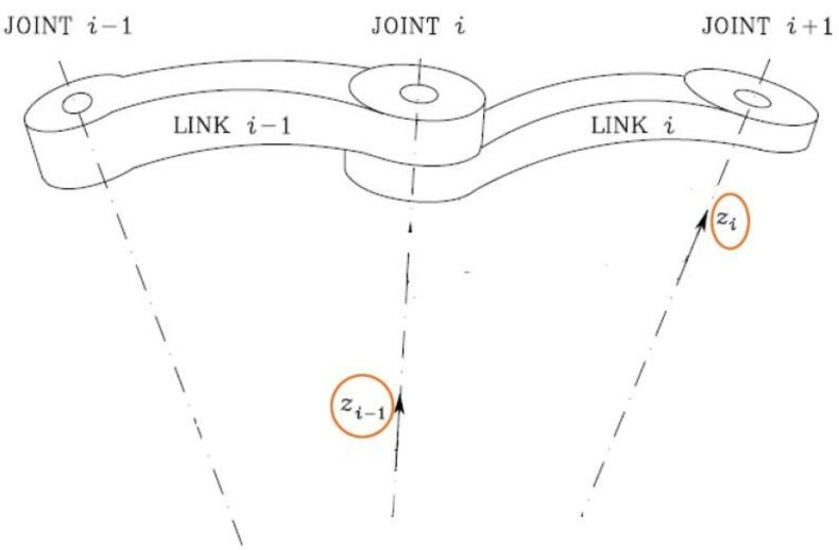
\includegraphics[width=0.8\linewidth]{DH_Images/DH_1.jpg}
        \end{center}
    \end{minipage}

    \item
    \begin{minipage}[t]{0.48\textwidth}
        L'origine \(O_{i}\) del sistema di riferimento \(i\) è posta all'intersezione dell'asse \(z_{i}\) con la normale comune agli assi \(z_{i-1}\) e \(z_{i}\).
    \end{minipage}
    \hfill
    \begin{minipage}[h]{0.48\textwidth}
        \begin{center}
            \centering
            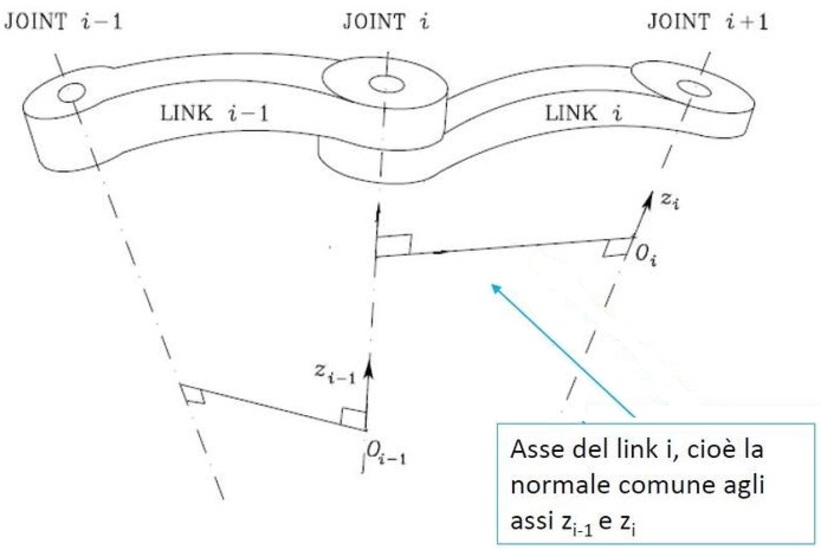
\includegraphics[width=0.8\linewidth]{DH_Images/DH_2.jpg}
        \end{center}
    \end{minipage}

    \item
    \begin{minipage}[t]{0.48\textwidth}
        L'asse \(x_{i}\) è allineato con la normale comune agli assi \(z_{i-1}\) e \(z_{i}\). Il verso positivo è orientato dal giunto \(i\) verso il giunto \(i+1\).
    \end{minipage}
    \hfill
    \begin{minipage}[h]{0.48\textwidth}
        \begin{center}
            \centering
            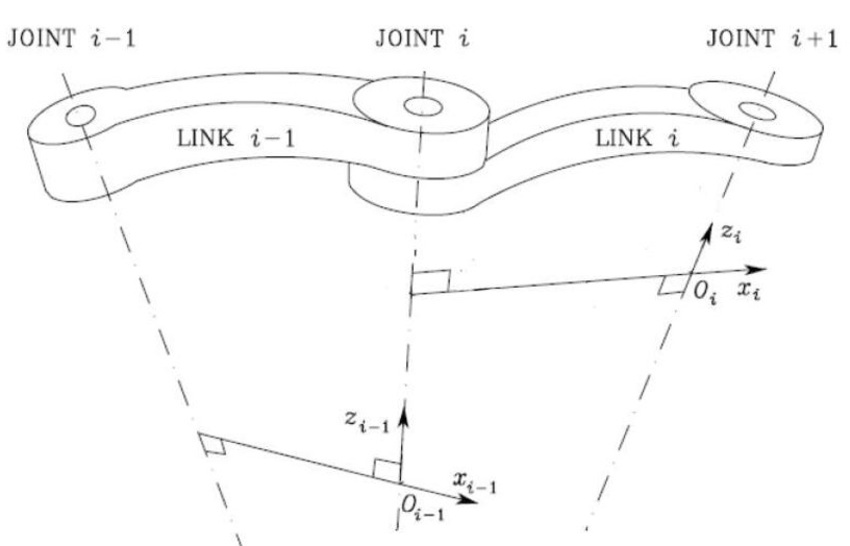
\includegraphics[width=0.75\linewidth]{DH_Images/DH_3.jpg}
        \end{center}
    \end{minipage}

    \item
    \begin{minipage}[t]{0.48\textwidth}
        L'asse \(y_{i}\) è definito in modo da completare una terna cartesiana destrogira, secondo la regola della mano destra (\(y_i = z_i \times x_i\)).
    \end{minipage}
    \hfill
    \begin{minipage}[h]{0.48\textwidth}
        \begin{center}
            \centering
            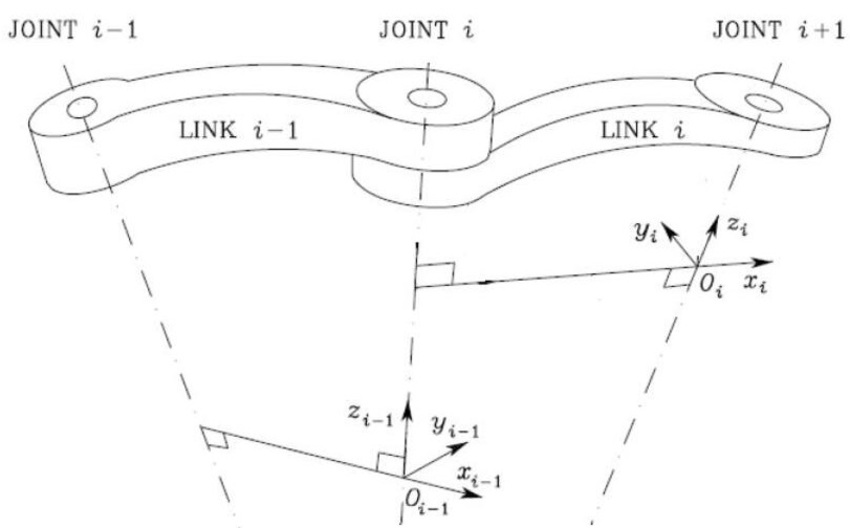
\includegraphics[width=0.75\linewidth]{DH_Images/DH_4.jpg}
        \end{center}
    \end{minipage}
\end{enumerate}
In questo modo, la terna \(i\) definisce il sistema di riferimento \(RF_{i}\) solidale al braccio \(i\).

Questa convenzione presenta alcuni casi di ambiguità, per i quali si seguono delle regole specifiche:
\begin{itemize}
    \item \textbf{Sistema di riferimento di base (\(RF_0\))}: Poiché non esiste un asse \(z_{-1}\), la scelta dell'origine \(O_0\) e della direzione dell'asse \(x_0\) è arbitraria. Tipicamente, \(RF_0\) è fissato alla base del robot.

    \item \textbf{Sistema di riferimento finale (\(RF_n\))}: Non esistendo il giunto \(n+1\), la direzione dell'asse \(z_n\) non è univocamente determinata e può essere scelta liberamente (spesso si allinea con \(z_{n-1}\)). Di conseguenza, la scelta di \(O_n\) e \(x_n\) gode di maggiore libertà.

    \item \textbf{Assi \(z_{i-1}\) e \(z_i\) paralleli}: Esistono infinite normali comuni. La scelta dell'origine \(O_{i}\) lungo l'asse \(z_{i}\) è quindi arbitraria.

    \item \textbf{Assi \(z_{i-1}\) e \(z_i\) incidenti}: La normale comune ha lunghezza nulla. In questo caso, l'asse \(x_{i}\) è definito come ortogonale al piano formato da \(z_{i-1}\) e \(z_i\), con verso dato da \(z_{i-1} \times z_i\).
\end{itemize}
\newpage

Una volta definiti i sistemi di riferimento \(RF_{i}\), la posa della terna \(i\) rispetto alla terna \(i-1\) è descritta da quattro parametri.

\begin{minipage}[h]{0.48\textwidth}
    \subsubsection*{Parametro \(\bm{a_{i}}\)}
    Rappresenta la distanza tra gli assi \(z_{i-1}\) e \(z_{i}\), misurata lungo l'asse \(x_i\). È un parametro fisso che dipende dalla geometria del braccio \(i\).
\end{minipage}
\hfill
\begin{minipage}[h]{0.48\textwidth}
    \begin{center}
        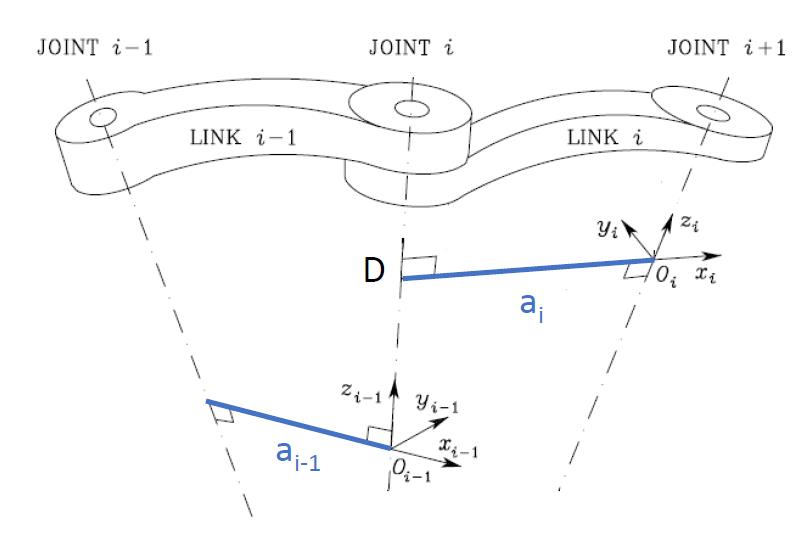
\includegraphics[width=0.75\linewidth]{DH_Images/DH_5.jpg}
    \end{center}
\end{minipage}

\vspace{1cm}

\begin{minipage}[h]{0.48\textwidth}
\subsubsection*{Parametro \(\bm{d_{i}}\)}
    Rappresenta la distanza tra gli assi \(x_{i-1}\) e \(x_{i}\), misurata lungo l'asse \(z_{i-1}\). Se il giunto \(i\) è prismatico, \(d_i\) è la variabile di giunto. Altrimenti, è un parametro fisso.
\end{minipage}
\hfill
\begin{minipage}[h]{0.48\textwidth}
    \begin{center}
        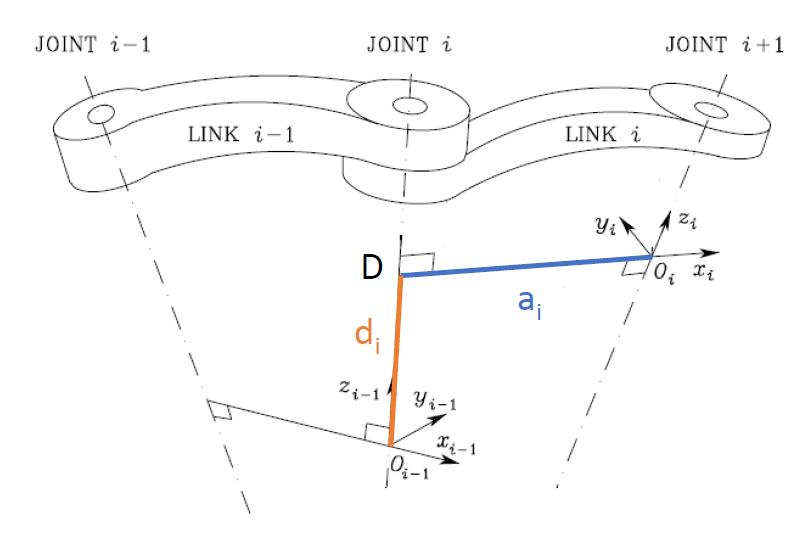
\includegraphics[width=0.75\linewidth]{DH_Images/DH_6.jpg}
    \end{center}
\end{minipage}

\vspace{1cm}

\begin{minipage}[h]{0.48\textwidth}
    \subsubsection*{Parametro \(\bm{\alpha_{i}}\)}
    Rappresenta l'angolo tra gli assi \(z_{i-1}\) e \(z_i\), misurato intorno all'asse \(x_i\). Questo parametro, detto \textit{twist}, è fisso e dipende dalla geometria del braccio \(i\). La convenzione del segno positivo è una rotazione antioraria da \(z_{i-1}\) a \(z_i\) vista lungo \(x_i\).
\end{minipage}
\hfill
\begin{minipage}[h]{0.48\textwidth}
    \begin{center}
        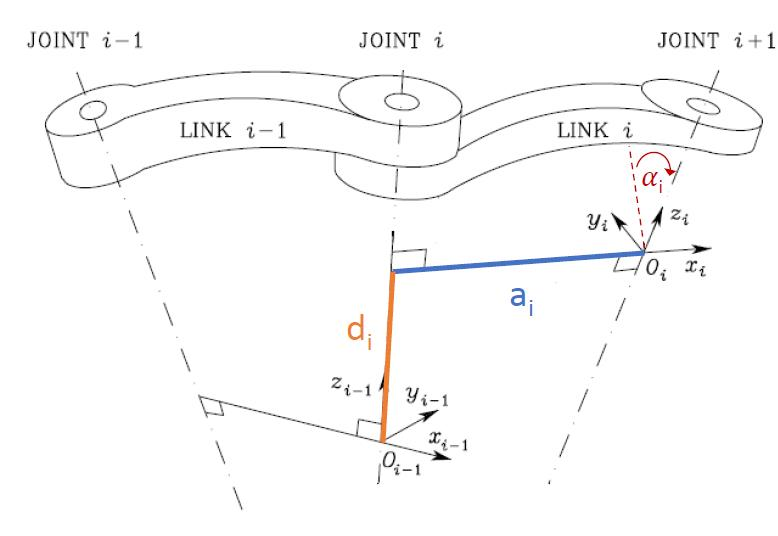
\includegraphics[width=0.75\linewidth]{DH_Images/DH_7.jpg}
    \end{center}
\end{minipage}

\vspace{1cm}

\begin{minipage}[h]{0.45\textwidth}
    \subsubsection*{Parametro \(\bm{\theta_{i}}\)}
    Rappresenta l'angolo tra gli assi \(x_{i-1}\) e \(x_i\), misurato intorno all'asse \(z_{i-1}\). Se il giunto \(i\) è rotoidale, \(\theta_i\) è la variabile di giunto. Altrimenti, è un parametro fisso. La convenzione del segno positivo è una rotazione antioraria da \(x_{i-1}\) a \(x_i\) vista lungo \(z_{i-1}\).
\end{minipage}
\hfill
\begin{minipage}[h]{0.45\textwidth}
    \begin{center}
        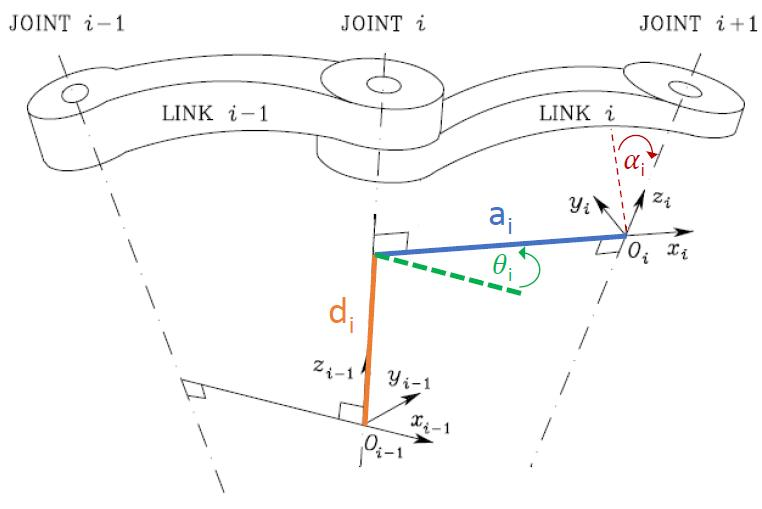
\includegraphics[width=0.75\textwidth]{DH_Images/DH_8.jpg}
    \end{center}
\end{minipage}

\newpage
I parametri DH (\(a_{i}\), \(d_{i}\), \(\alpha_{i}\), \(\theta_{i}\)) permettono di definire la trasformazione omogenea per passare dal sistema di riferimento \(i-1\) al sistema \(i\) attraverso due passaggi elementari.

\begin{itemize}
    \item \textbf{Passaggio 1: Trasformazione lungo e attorno a \(z_{i-1}\)}\\
    Si definisce una terna intermedia \(i'\) applicando una rotazione di angolo \(\theta_i\) e una traslazione di distanza \(d_i\) rispetto all'asse \(z_{i-1}\).
    \begin{center}
        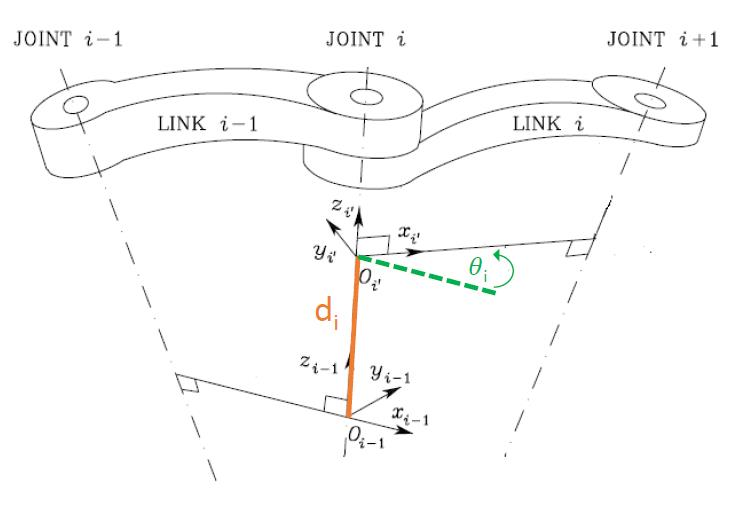
\includegraphics[width=0.5\textwidth]{DH_Images/DH_9.jpg}
    \end{center}
    La matrice di trasformazione omogenea $^{i-1}\bm{A}_{i'}(q_i)$ è data dal prodotto di una rotazione e una traslazione:
    \[
        ^{i-1}\bm{A}_{i'}(q_i) = \text{Rot}(z_{i-1}, \theta_i) \cdot \text{Trasl}(z_{i-1}, d_i) =
        \begin{bmatrix}
            \cos(\theta_i) & -\sin(\theta_i) & 0 & 0 \\
            \sin(\theta_i) & \cos(\theta_i) & 0 & 0 \\
            0 & 0 & 1 & d_i \\
            0 & 0 & 0 & 1
        \end{bmatrix}
    \]
\end{itemize}

\begin{itemize}
    \item \textbf{Passaggio 2: Trasformazione lungo e attorno a \(x_{i}\)}\\
    Dalla terna intermedia \(i'\), si ottiene la terna finale \(i\) applicando una traslazione di distanza \(a_i\) e una rotazione di angolo \(\alpha_i\) rispetto all'asse \(x_i\).
    \begin{center}
        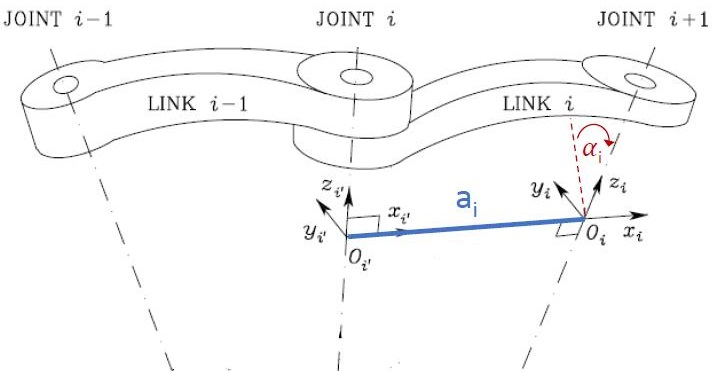
\includegraphics[width=0.5\textwidth]{DH_Images/DH_10.jpg}
    \end{center}
    La matrice corrispondente, \(^{i'}\bm{A}_{i}\), è:
    \[
        ^{i'}\bm{A}_{i} = \text{Trasl}(x_{i}, a_i) \cdot \text{Rot}(x_{i}, \alpha_i) =
        \begin{bmatrix}
            1 & 0 & 0 & a_{i}\\
            0 & \cos(\alpha_i) & -\sin(\alpha_i) & 0 \\
            0 & \sin(\alpha_i) & \cos(\alpha_i) & 0 \\
            0 & 0 & 0 & 1 \\
        \end{bmatrix}
    \]
\end{itemize}

\noindent Svolgendo il prodotto matriciale $^{i - 1}\bm{A}_{i}(q_{i}) = \; ^{i - 1}\bm{A}_{i'}(q_{i}) \cdot {^{i'}\bm{A}_{i}}$, si ottiene la matrice di trasformazione completa di Denavit-Hartenberg:
\[
    ^{i - 1}\bm{A}_{i}(q_{i}) =
    \begin{bmatrix}
        \cos(\theta_i) & -\sin(\theta_i)\cos(\alpha_{i}) & \sin(\theta_i)\sin(\alpha_{i}) & a_{i}\cos(\theta_{i})\\
        \sin(\theta_i) & \cos(\theta_i)\cos(\alpha_{i}) & -\cos(\theta_i)\sin(\alpha_{i}) & a_{i}\sin(\theta_{i})\\
        0 & \sin(\alpha_{i}) & \cos(\alpha_{i}) & d_{i}\\
        0 & 0 & 0 & 1
    \end{bmatrix}
\]
\newpage
Una volta definita la matrice di trasformazione omogenea \(^{i-1}\mathbf{A}_{i}\) per un singolo link, è possibile risolvere il problema della cinematica diretta, ovvero determinare la posa (posizione e orientamento) dell'organo terminale (end-effector) rispetto al sistema di riferimento di base (\(RF_0\)).

È fondamentale notare che la matrice \(^{i-1}\mathbf{A}_{i}\) è funzione di un'unica variabile di giunto \(q_i\), mentre i restanti tre parametri DH sono costanti definite dalla geometria del manipolatore.
\[
    q_{i} =
    \begin{cases}
        \theta_{i} \qquad&\text{se il giunto è rotoidale}\\
        d_{i} \qquad&\text{se il giunto è prismatico}\\
    \end{cases}
\]
Per ottenere la posa finale dell'end-effector (solidale al sistema \(RF_n\)) rispetto alla base (\(RF_0\)), si moltiplicano in catena le singole matrici di trasformazione, dalla base fino all'ultimo giunto:
\[
    ^{0}\bm{T}_{n} = {^{0}\bm{A}_{1}(q_{1})} \cdot {^{1}\bm{A}_{2}(q_{2})} \cdot \dots \cdot {^{n-1}\bm{A}_{n}(q_{n})}
\]
La matrice risultante $^{0}\bm{T}_{n}$ contiene la descrizione completa della posa dell'end-effector. In particolare, il vettore posizione della sua origine, denotato con $^{0}\bm{P}_{EE}$, corrisponde alla quarta colonna della matrice. Matematicamente, questo è equivalente al calcolo:
\[
    \begin{bmatrix}
        ^{0}\bm{P}_{EE} \\
        1
    \end{bmatrix}
    = {^{0}\bm{T}_{n}} \cdot
    \begin{bmatrix}
        0 \\ 0 \\ 0 \\ 1
    \end{bmatrix}
\]



\newpage
% --- Riga 1 ---
\begin{minipage}[t]{0.48\textwidth}
    \subsubsection*{Manipolatore RR}
    \centering
    \begin{tabular}{|c|c|c|c|c|}
        \hline
        \textbf{\# Link} & \(\boldsymbol{\theta}\) & \(\boldsymbol{d}\) & \(\boldsymbol{\alpha}\) & \(\boldsymbol{a}\) \\
        \hline
        1 & \(q_{1}\) & 0 & 0 & \(a_{1}\) \\
        \hline
        2 & \(q_{2}\) & 0 & 0 & \(a_{2}\) \\
        \hline
    \end{tabular}
\end{minipage}
\hfill
\begin{minipage}[t]{0.48\textwidth}
    \subsubsection*{Manipolatore RRR}
    \centering
    \begin{tabular}{|c|c|c|c|c|}
        \hline
        \textbf{\# Link} & \(\boldsymbol{\theta}\) & \(\boldsymbol{d}\) & \(\boldsymbol{\alpha}\) & \(\boldsymbol{a}\) \\
        \hline
        1 & \(q_{1}\) & 0 & 0 & \(a_{1}\) \\
        \hline
        2 & \(q_{2}\) & 0 & 0 & \(a_{2}\) \\
        \hline
        3 & \(q_{3}\) & 0 & 0 & \(a_{3}\) \\
        \hline
    \end{tabular}
\end{minipage}

\vspace{1cm} % Spazio verticale tra le righe di minipage

% --- Riga 2 ---
\begin{minipage}[t]{0.48\textwidth}
    \subsubsection*{Manipolatore RPR}
    \centering
    \begin{tabular}{|c|c|c|c|c|}
        \hline
        \textbf{\# Link} & \(\boldsymbol{\theta}\) & \(\boldsymbol{d}\) & \(\boldsymbol{\alpha}\) & \(\boldsymbol{a}\) \\
        \hline
        1 & \(q_{1}\) & 0 & \(\frac{\pi}{2}\) & 0\\
        \hline
        2 & \(\frac{\pi}{2}\) & \(q_{2}\) & \(-\frac{\pi}{2}\) & 0\\
        \hline
        3 & \(q_{3}\) & 0 & 0 & 0\\
        \hline
    \end{tabular}
\end{minipage}
\hfill
\begin{minipage}[t]{0.48\textwidth}
    \subsubsection*{Manipolatore SCARA}
    \centering
    \begin{tabular}{|c|c|c|c|c|}
        \hline
        \textbf{\# Link} & \(\boldsymbol{\theta}\) & \(\boldsymbol{d}\) & \(\boldsymbol{\alpha}\) & \(\boldsymbol{a}\) \\
        \hline
        1 & \(q_{1}\) & \(d_{1}\) & 0 & \(a_{1}\) \\
        \hline
        2 & \(q_{2}\) & 0 & \(\pi\) & \(a_{2}\) \\
        \hline
        3 & 0 & \(q_{3}\) & 0 & 0 \\
        \hline
        4 & \(q_{4}\) & \(d_{4}\) & 0 & 0 \\
        \hline
    \end{tabular}

\end{minipage}

\vspace{1cm} % Spazio verticale tra le righe di minipage

% --- Riga 3 ---
\begin{minipage}[t]{0.48\textwidth}
    \subsubsection*{Manipolatore Cilindrico}
    \centering
    \begin{tabular}{|c|c|c|c|c|}
        \hline
        \textbf{\# Link} & \(\boldsymbol{\theta}\) & \(\boldsymbol{d}\) & \(\boldsymbol{\alpha}\) & \(\boldsymbol{a}\) \\
        \hline
        1 & \(q_{1}\) & \(d_{1}\) & 0 & 0 \\
        \hline
        2 & \(-\frac{\pi}{2}\) & \(q_{2}\) & \(\frac{\pi}{2}\) & 0\\
        \hline
        3 & 0 & \(q_{3}\) & 0 & 0 \\
        \hline
    \end{tabular}

\end{minipage}
\hfill
\begin{minipage}[t]{0.48\textwidth}
    \subsubsection*{Manipolatore Sferico}
    \centering
    \begin{tabular}{|c|c|c|c|c|}
        \hline
        \textbf{\# Link} & \(\boldsymbol{\theta}\) & \(\boldsymbol{d}\) & \(\boldsymbol{\alpha}\) & \(\boldsymbol{a}\) \\
        \hline
        1 & \(q_{1}\) & \(d_{1}\) & \(\frac{\pi}{2}\) & 0 \\
        \hline
        2 & \(q_{2}\) & 0 & \(-\frac{\pi}{2}\) & 0\\
        \hline
        3 & 0 & \(q_{3}\) & 0 & 0 \\
        \hline
    \end{tabular}
\end{minipage}

\vspace{1cm} % Spazio verticale tra le righe di minipage

% --- Riga 4 (NUOVA) ---
\begin{minipage}[t]{0.48\textwidth}
    \subsubsection*{Manipolatore di Stanford}
    \centering
    \begin{tabular}{|c|c|c|c|c|}
        \hline
        \textbf{\# Link} & \(\boldsymbol{\theta}\) & \(\boldsymbol{d}\) & \(\boldsymbol{\alpha}\) & \(\boldsymbol{a}\) \\
        \hline
        1 & \(q_{1}\) & \(d_{1}\) & \(-\frac{\pi}{2}\) & 0 \\
        \hline
        2 & \(q_{2}\) & \(d_{2}\) & \(\frac{\pi}{2}\) & 0 \\
        \hline
        3 & 0 & \(q_{3}\) & 0 & 0 \\
        \hline
        4 & \(q_{4}\) & 0 & \(-\frac{\pi}{2}\) & 0 \\
        \hline
        5 & \(q_{5}\) & 0 & \(\frac{\pi}{2}\) & 0 \\
        \hline
        6 & \(q_{6}\) & \(d_{6}\) & 0 & 0 \\
        \hline
    \end{tabular}
\end{minipage}
\hfill
\begin{minipage}[t]{0.48\textwidth}
    \subsubsection*{Manipolatore Antropomorfo (6R)}
    \centering
    \begin{tabular}{|c|c|c|c|c|}
        \hline
        \textbf{\# Link} & \(\boldsymbol{\theta}\) & \(\boldsymbol{d}\) & \(\boldsymbol{\alpha}\) & \(\boldsymbol{a}\) \\
        \hline
        1 & \(q_{1}\) & 0 & \(-\frac{\pi}{2}\) & 0 \\
        \hline
        2 & \(q_{2}\) & 0 & 0 & \(a_{2}\) \\
        \hline
        3 & \(q_{3}\) & 0 & \(-\frac{\pi}{2}\) & \(a_{3}\) \\
        \hline
        4 & \(q_{4}\) & \(d_{4}\) & \(\frac{\pi}{2}\) & 0 \\
        \hline
        5 & \(q_{5}\) & 0 & \(-\frac{\pi}{2}\) & 0 \\
        \hline
        6 & \(q_{6}\) & \(d_{6}\) & 0 & 0 \\
        \hline
    \end{tabular}
\end{minipage}

\newpage


\subsubsection*{Esempio: Posizione dell'End-Effector del Manipolatore RPR}

Applichiamo il metodo generale al manipolatore RPR. Le matrici di trasformazione omogenea per ciascun giunto sono:
\begin{align*}
    ^{0}\bm{A}_{1}(q_{1}) &=
    \begin{bmatrix}
        \cos(q_{1}) & 0 & -\sin(q_{1}) & 0\\
        \sin(q_{1}) & 0 & \cos(q_{1}) & 0\\
        0 & -1 & 0 & A\\
        0 & 0 & 0 & 1
    \end{bmatrix} \\
    ^{1}\bm{A}_{2}(q_{2}) &=
    \begin{bmatrix}
        0 & 0 & 1 & 0\\
        -1 & 0 & 0 & 0\\
        0 & -1 & 0 & q_{2}\\
        0 & 0 & 0 & 1
    \end{bmatrix} \\
    ^{2}\bm{A}_{3}(q_{3}) &=
    \begin{bmatrix}
        \cos(q_{3}) & -\sin(q_{3}) & 0 & B\cos(q_{3})\\
        \sin(q_{3}) & \cos(q_{3}) & 0 & B\sin(q_{3})\\
        0 & 0 & 1 & 0\\
        0 & 0 & 0 & 1
    \end{bmatrix}
\end{align*}

La matrice di trasformazione totale dalla base all'end-effector è $^{0}\bm{T}_{3} = {^{0}\bm{A}_{1}} \cdot {^{1}\bm{A}_{2}} \cdot {^{2}\bm{A}_{3}}$. Eseguendo il prodotto:
\[
    ^{0}\bm{T}_{3} =
    \begin{bmatrix}
        \cos(q_1) & 0 & -\sin(q_1) & 0 \\
        \sin(q_1) & 0 & \cos(q_1) & 0 \\
        0 & -1 & 0 & A \\
        0 & 0 & 0 & 1
    \end{bmatrix}
    \begin{bmatrix}
        - \sin(q_3) & - \cos(q_3) & 0 & - B \sin(q_3) \\
        - \cos(q_3) & \sin(q_3) & 0 & B \cos(q_3) \\
        0 & 0 & -1 & -q_2 \\
        0 & 0 & 0 & 1
    \end{bmatrix}
\]
\[
    ^{0}\bm{T}_{3} =
    \begin{bmatrix}
        -\cos(q_1)\sin(q_3) & -\cos(q_1)\cos(q_3) & \sin(q_1) & B\sin(q_1)\sin(q_3) - q_2\sin(q_1) \\
        -\sin(q_1)\sin(q_3) & -\sin(q_1)\cos(q_3) & -\cos(q_1) & -B\cos(q_1)\sin(q_3) + q_2\cos(q_1) \\
        \cos(q_3) & -\sin(q_3) & 0 & A+B\cos(q_3) \\
        0 & 0 & 0 & 1
    \end{bmatrix}
\]
Il vettore posizione dell'origine dell'end-effector (\(EE\)) rispetto alla base è la quarta colonna di $^{0}\bm{T}_{3}$:
\[
    ^{0}\bm{P}_{EE} =
    \begin{bmatrix}
        B\sin(q_{1})\sin(q_{3}) - q_{2}\sin(q_{1}) \\
        q_{2}\cos(q_{1}) - B\cos(q_{1})\sin(q_{3}) \\
        A + B\cos(q_{3})
    \end{bmatrix}
\]
\newpage
\subsubsection{Singolarità Cinematiche}

Le singolarità cinematiche sono configurazioni specifiche di un manipolatore in cui la sua capacità di muoversi o di esercitare forze in determinate direzioni nello spazio operativo è ridotta. In queste pose, il robot perde uno o più gradi di libertà, e la mappatura tra lo spazio dei giunti e lo spazio operativo cessa di essere biunivoca.

Dal punto di vista del problema cinematico inverso, una singolarità si manifesta come l'impossibilità di determinare in modo univoco le variabili di giunto necessarie per raggiungere una data posa dell'end-effector. Questo fenomeno è spesso noto come \textbf{gimbal lock}, dove due assi di rotazione del robot si allineano, rendendo i loro effetti indistinguibili.

\subsubsection*{Analisi Singolarità Di Rappresentazione}
Per analizzare questa condizione, si consideri un orientamento dell'end-effector descritto da una sequenza di tre rotazioni elementari, come gli angoli di Eulero XYZ:
\[
    \mathbf{R}(\phi, \theta, \psi) = \mathbf{R}_{X}(\phi) \mathbf{R}_{Y}(\theta) \mathbf{R}_{Z}(\psi)
\]
L'obiettivo è dimostrare che questa rappresentazione diventa singolare per un valore critico di \(\theta\). Per farlo, si sfrutta un'identità che permette di esprimere una rotazione attorno a un asse tramite rotazioni attorno ad altri due. Nello specifico, la rotazione attorno all'asse \(x\) può essere riscritta come:
\[
    \mathbf{R}_{X}(\phi) = \mathbf{R}_{Y}\left(\frac{\pi}{2}\right) \mathbf{R}_{Z}(\phi) \mathbf{R}_{Y}\left(-\frac{\pi}{2}\right)
\]
Sostituendo questa espressione nella formula dell'orientamento, si raggruppano i termini per analizzarne l'interazione:
\[
    \mathbf{R}(\phi, \theta, \psi) = \left[ \mathbf{R}_{Y}\left(\frac{\pi}{2}\right) \mathbf{R}_{Z}(\theta) \mathbf{R}_{Y}\left(-\frac{\pi}{2}\right) \right] \mathbf{R}_{Y}(\theta) \mathbf{R}_{Z}(\psi)
\]
Si esamina ora il caso particolare in cui il giunto intermedio assume il valore critico \( \theta = \frac{\pi}{2} \). La parte centrale dell'espressione diventa il prodotto di due rotazioni opposte attorno allo stesso asse \(Y\), che si annullano a vicenda (risultando nella matrice identità \(\mathbf{I}\)):
\[
    \mathbf{R}_{Y}\left(-\frac{\pi}{2}\right) \mathbf{R}_{Y}\left(\frac{\pi}{2}\right) = \mathbf{I}
\]
La matrice di rotazione totale si semplifica drasticamente:
\begin{align*}
    \mathbf{R}\left(\phi, \frac{\pi}{2}, \psi\right) &= \mathbf{R}_{Y}\left(\frac{\pi}{2}\right) \mathbf{R}_{Z}(\phi) \left[ \mathbf{R}_{Y}\left(-\frac{\pi}{2}\right) \mathbf{R}_{Y}\left(\frac{\pi}{2}\right) \right] \mathbf{R}_{Z}(\psi) \\
    &= \mathbf{R}_{Y}\left(\frac{\pi}{2}\right) \mathbf{R}_{Z}(\phi) \mathbf{I} \mathbf{R}_{Z}(\psi) \\
    &= \mathbf{R}_{Y}\left(\frac{\pi}{2}\right) \left[ \mathbf{R}_{Z}(\phi) \mathbf{R}_{Z}(\psi) \right] \\
    &= \mathbf{R}_{Y}\left(\frac{\pi}{2}\right) \mathbf{R}_{Z}(\phi + \psi)
\end{align*}

Il risultato finale \(\mathbf{R} = \mathbf{R}_{Y}(\frac{\pi}{2}) \mathbf{R}_{Z}(\phi + \psi)\), mostra che l'orientamento dell'end-effector non dipende più individualmente da \(\phi\) e \(\psi\), ma solo dalla loro \textbf{somma}. Questo significa che infinite combinazioni dei due angoli producono lo stesso identico orientamento. Ad esempio, se \(\phi + \psi = 45^\circ\), le coppie \((45^\circ, 0^\circ)\), \((30^\circ, 15^\circ)\) e \((0^\circ, 45^\circ)\) sono tutte soluzioni valide per lo stesso problema cinematico inverso.

Questa singolarità ha implicazioni significative e problematiche nel controllo del manipolatore:
\begin{itemize}
    \item \textbf{Ambiguità Cinematica Inversa:} In una configurazione singolare esistono infinite soluzioni per i giunti, rendendo impossibile sceglierne una in modo univoco.

    \item \textbf{Instabilità Controllo:} In prossimità di una singolarità, la matrice Jacobiana del manipolatore diventa singolare. Ciò implica che per generare piccole variazioni di velocità dell'end-effector in certe direzioni, sarebbero necessarie velocità di giunto teoricamente infinite. Questo può portare a movimenti incontrollati e potenziali danni al robot.

    \item \textbf{Complessità Nella Pianificazione Della Traiettoria:} I percorsi dell'end-effector devono essere pianificati attentamente per evitare di attraversare o avvicinarsi a configurazioni singolari.
\end{itemize}

\newpage
\section{Cinematica Inversa}
La \textbf{cinematica inversa} di un robot definisce il problema di calcolare i valori delle variabili di giunto, indicati con \( \mathbf{q} \), necessari affinché l'End Effector raggiunga una determinata posizione e orientamento nello spazio. A differenza della cinematica diretta, che determina la posa dell'end-effector a partire dai valori dei giunti, il problema inverso è notevolmente più complesso per diverse ragioni. Le principali criticità sono:

\begin{enumerate}
    \item \textbf{Non Linearità Delle Equazioni}: Le equazioni matematiche che governano la cinematica inversa sono non lineari. Di conseguenza, trovare una soluzione analitica in forma chiusa è spesso impossibile, rendendo necessario il ricorso a metodi numerici o approssimati per la loro risoluzione.

    \item \textbf{Soluzioni Multiple}: Per una singola posizione e orientamento dell'end-effector, possono esistere molteplici configurazioni dei giunti che soddisfano la richiesta. Questa molteplicità di soluzioni richiede la scelta di quella più ottimale, basata su criteri come il consumo di energia o la minimizzazione degli spostamenti.

    \item \textbf{Infinite Soluzioni Per Manipolatori Ridondanti}: Un manipolatore è definito \textit{ridondante} quando possiede un numero di gradi di libertà superiore a quello strettamente necessario per compiere un'operazione. In tali casi, il problema della cinematica inversa ammette un numero infinito di soluzioni, poiché esistono innumerevoli configurazioni dei giunti in grado di realizzare la stessa posa finale.

    \item \textbf{Assenza Di Soluzioni Ammissibili}: È possibile che non esista alcuna configurazione di giunto in grado di raggiungere la posa desiderata. Questo si verifica quando il punto target si trova al di fuori dello spazio di lavoro del robot, a causa di limitazioni fisiche e geometriche intrinseche alla sua struttura.
\end{enumerate}

La risoluzione della cinematica inversa rappresenta una sfida fondamentale in robotica e viene affrontata con diversi approcci, tra cui metodi analitici, numerici, scelti in base alla complessità del manipolatore. In sintesi, data la posa desiderata dell'organo terminale, espressa dalla matrice di trasformazione omogenea:
\[
    \bm{T} =
    \begin{bmatrix}
        \bm{R} & \bm{P}\\
        \bm{0}_{1\times 3} & 1
    \end{bmatrix}
\]
L'obiettivo è determinare un vettore di variabili di giunto \( \mathbf{q} \) tale che la matrice di trasformazione calcolata dalla cinematica diretta, \(^{0}\bm{A}_{n}(\mathbf{q})\), coincida con \(\bm{T}\).

Le principali sfide di questo problema includono:
\begin{itemize}
    \item La necessità di risolvere equazioni non lineari, per le quali non sempre esiste una soluzione analitica.
    \item La possibilità che le equazioni ammettano soluzioni multiple o infinite.
    \item L'eventualità che, a causa della struttura del manipolatore, non esistano soluzioni ammissibili.
\end{itemize}


\newpage
\subsection{Spazio dei Giunti e Spazio di Lavoro}
Per analizzare l'esistenza di soluzioni al problema della cinematica inversa, si definiscono due insiemi fondamentali che caratterizzano lo spazio di lavoro di un manipolatore:

\begin{itemize}
    \item \textbf{Workspace Primario \( W_{S1} \) (Spazio Raggiungibile)}: È l'insieme di tutti i punti \( p \) che l'end-effector del manipolatore è in grado di raggiungere con \textit{almeno un} orientamento \( \phi \) (o una rotazione \( R \)). Se un punto si trova al di fuori di questo spazio, il problema della cinematica inversa non ammette soluzioni. Al contrario, se un punto \( p \) appartiene a \( W_{S1} \), esiste almeno una configurazione dei giunti che permette di raggiungerlo.
        \begin{flalign*}
            & WS_{1} = \biggl\{ p \in \mathbb{R}^{3} \; : \; \exists \, q \; : \; f(q) = p\biggr\}\\
            & p \; \notin \; WS_{1} \quad\longrightarrow\quad \nexists \; q\\
            & p \; \in \; WS_{1} \quad\longrightarrow\quad \exists \; q
        \end{flalign*}

    \item \textbf{Workspace Secondario \( W_{S2} \) (Spazio di Destrezza)}: È l'insieme dei punti \( p \) che l'end-effector può raggiungere con \textit{qualsiasi} orientamento fisicamente realizzabile. Un punto appartenente a \( W_{S2} \) garantisce la massima destrezza del manipolatore, poiché la sua posizione può essere raggiunta con un'orientazione arbitraria.
    \[
        WS_{2} = \biggl\{ p \in \mathbb{R}^{3} \; : \forall \, \bm{R} \in SO(3) \; \exists \, q \; : \; ^{0}A_{n}(q) =
        \begin{bmatrix}
            \bm{R} & \bm{p}\\
            \bm{0}_{1\times 3} & 1
        \end{bmatrix}
        \biggr\}
    \]
\end{itemize}

Per definizione, lo Spazio di Destrezza è un sottoinsieme dello Spazio Raggiungibile (\( W_{S2} \subseteq W_{S1} \)). Lo spazio di lavoro complessivo del manipolatore è determinato dalla sua geometria e dai vincoli meccanici imposti sui suoi giunti.

La risolvibilità del problema della cinematica inversa è garantita solo se la posa desiderata (posizione e orientamento) appartiene allo spazio di lavoro del manipolatore.

\subsubsection*{Esempio}
Consideriamo un manipolatore planare \textbf{RR} (due giunti rotoidali). I suoi spazi di lavoro primario e secondario dipendono dalla relazione tra le lunghezze dei suoi due bracci, \( l_1 \) e \( l_2 \).

\paragraph{Caso 1: \(l_1 \neq l_2\)}
In questa configurazione, gli spazi di lavoro sono definiti come segue:
\begin{itemize}
    \item \textbf{Spazio Operativo Primario (\(WS_1\))}: È una corona circolare centrata nell'origine, con raggio interno \(|l_1 - l_2|\) e raggio esterno \(l_1 + l_2\). Questi limiti rappresentano, rispettivamente, la minima e la massima distanza che l'end-effector può raggiungere dall'origine.
    $$
        WS_{1} = \big\{ p \in \mathbb{R}^2 : |l_{1} - l_{2}| \leq \|p\| \leq l_{1} + l_{2} \big\}.
    $$

    \item \textbf{Spazio Operativo Secondario (\(WS_2\))}: È l'insieme vuoto, poiché non esiste alcun punto che possa essere raggiunto con un orientamento arbitrario.
    $$
    WS_2 = \emptyset.
    $$
\end{itemize}

\paragraph{Caso 2: \(l_1 = l_2 = l\)}
Quando i due bracci hanno la stessa lunghezza, gli spazi di lavoro cambiano come segue:
\begin{itemize}
    \item \textbf{Spazio Operativo Primario (\(WS_1\))}: Diventa un disco pieno centrato nell'origine con raggio \(2l\). La distanza massima è la somma delle lunghezze (\(l+l=2l\)), mentre la minima è zero, ottenibile quando i bracci sono ripiegati l'uno sull'altro.
    $$
    WS_1 = \big\{ p \in \mathbb{R}^2 : \|p\| \leq 2l \big\}.
    $$

    \item \textbf{Spazio Operativo Secondario (\(WS_2\))}: Si riduce al solo punto di origine. L'origine è l'unico punto che può essere raggiunto con qualsiasi orientamento dell'end-effector.
    $$
    WS_2 = \{0\}.
    $$
\end{itemize}

\newpage
\subsection{Cinematica Manipolatore RR Planare}

\begin{minipage}[c]{0.45\textwidth}
    Lo spazio operativo rappresenta tutte le posizioni e orientazioni che l'utensile (end-effector) può raggiungere. In questo caso, lo spazio operativo ha dimensione $m = 3$ ed è descritto dal vettore:
    \[
        \mathbf{r} =
        \begin{bmatrix}
        P_x \\
        P_y \\
        \phi
        \end{bmatrix}
    \]
    Dove  $P_x$ e $P_y$ sono le coordinate cartesiane dell'end-effector nel piano e $\phi$ è l'orientazione dell'end-effector rispetto all'asse orizzontale positivo.

    Le variabili di giunto descrivono le configurazioni del manipolatore. In questo caso, la dimensione delle variabili di giunto è $n = 2$ e sono descritte dal vettore:
    \[
        \mathbf{q} =
        \begin{bmatrix}
        q_1 \\
        q_2
        \end{bmatrix}
    \]
    Dove $q_1$ è l'angolo del primo braccio rispetto all'asse orizzontale e $q_2$ è l'angolo relativo tra il primo e il secondo braccio
\end{minipage}
\hfill
\begin{minipage}[c]{0.45\textwidth}
    \centering
    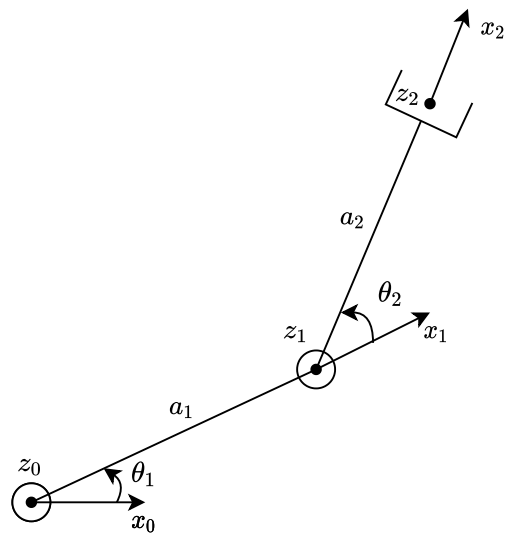
\includegraphics[width=0.9\linewidth]{RR_Planare.png}
\end{minipage}


\subsubsection{Cinematica Diretta}
Un robot planare con due giunti rotazionali (RR) ha il primo braccio di lunghezza \( l_1 \), il cui estremo si trova a una distanza \( l_1 \) dall'origine e forma un angolo \( q_1 \) rispetto all'asse orizzontale. Le sue coordinate cartesiane sono quindi:
\[
    x_1 = l_1 \cos q_1 \qquad y_1 = l_1 \sin q_1.
\]
L'end-effector è situato all'estremità del secondo braccio, che ha lunghezza \( l_2 \) e forma un angolo totale di \( q_1 + q_2 \) rispetto all'asse orizzontale. Le sue coordinate cartesiane sono date da:
\[
    P_x = x_1 + l_2 \cos (q_1 + q_2) \qquad P_y = y_1 + l_2 \sin (q_1 + q_2).
\]

Sostituendo le espressioni di \( x_1 \) e \( y_1 \), si ottiene la formulazione completa della cinematica diretta:
\[
    P_x = l_1 \cos q_1 + l_2 \cos (q_1 + q_2) \qquad
    P_y = l_1 \sin q_1 + l_2 \sin (q_1 + q_2).
\]

L'orientazione dell'end-effector è data dalla somma degli angoli dei due giunti:
\[
    \phi = q_1 + q_2.
\]

Pertanto, la posizione e l'orientazione dell'end-effector possono essere espresse in forma vettoriale come:
\[
    \mathbf{r} = f(q) =
    \begin{bmatrix}
        P_x \\
        P_y \\
        \phi
    \end{bmatrix}
    =
    \begin{bmatrix}
        l_1 \cos(q_1) + l_2 \cos (q_1 + q_2) \\
        l_1 \sin(q_1) + l_2 \sin (q_1 + q_2) \\
        q_1 + q_2
    \end{bmatrix}.
\]

\newpage
\subsubsection{Cinematica Inversa}
Dai risultati della cinematica diretta si nota che
\[
    x^{2} + y^{2} = \biggl[ l_1 \cos(q_1) + l_2 \cos (q_1 + q_2) \biggr]^{2} + \biggl[ l_1 \sin(q_1) + l_2 \sin (q_1 + q_2) \biggr]^{2} =
\]
\[
    = \biggl[ l_{1}^{2} \cos^{2}(q_1) + 2\biggl( l_{1} \cos (q_1) \biggr)\biggl(l_{2} \cos (q_1 + q_2)\biggr) + l_{2}^{2} \cos^{2} (q_1 + q_2) \biggr] +
\]
\[
    + \biggl[ l_{1}^{2} \sin^{2}(q_1) + 2\biggl( l_1 \sin(q_1) \biggr) \biggl( l_2 \sin (q_1 + q_2) \biggr) + l_{2}^{2} \sin^{2} (q_1 + q_2) \biggr] =
\]
\[
    = l_{1}^{2}\biggl[ \cos^{2}(q_1) + \sin^{2}(q_1) \biggr] + 2l_{1}l_{2}\biggl[ \cos (q_1)\cos (q_1 + q_2) + \sin(q_1)\sin(q_1 + q_2) \biggr] + l_{2}^{2}\biggl[ \cos^{2}(q_1 + q_2) + \sin^{2}(q_1 + q_2) \biggr] =
\]
Ricordando che \(\cos^{2}(\theta) + \sin^{2}(\theta) = 1\), si ottiene
\[
    = l_{1}^{2} + 2l_{1}l_{2}\biggl[ \cos (q_1)\cos (q_1 + q_2) + \sin(q_1)\sin(q_1 + q_2) \biggr] + l_{2}^{2}
\]
Quindi, si ottiene che
\[
    x^{2} + y^{2} = l_{1}^{2} + l_{2}^{2} + 2l_{1}l_{2}\biggl[ \cos (q_1)\cos (q_1 + q_2) + \sin(q_1)\sin(q_1 + q_2) \biggr]
\]
\[
    x^{2} + y^{2} - \biggr( l_{1}^{2} + l_{2}^{2} \biggl) =  2l_{1}l_{2}\biggl[ \cos (q_1)\cos (q_1 + q_2) + \sin(q_1)\sin(q_1 + q_2) \biggr]
\]
Ricordando la formula
\[
    \cos(\theta - \phi) = \cos(\theta)\cos(\phi) + \sin(\theta)\sin(\phi)
\]
E ponendo \(\theta = q_{1}\) e \(\phi = q_{1} + q_{2}\), quindi si può scrivere come
\[
    x^{2} + y^{2} - \biggr( l_{1}^{2} + l_{2}^{2} \biggl) =  2l_{1}l_{2} \cos\bigg[ q_{1} - \biggl(q_{1} + q_{2}\biggr) \biggr]
\]\[
    x^{2} + y^{2} - \biggr( l_{1}^{2} + l_{2}^{2} \biggl) =  2l_{1}l_{2} \cos\big( - q_{2}\ \bigr)
\]
Sapendo che il coseno è pari si ha che \(\cos(-q_2) = \cos(q_2)\) e di conseguenza
\[
    x^{2} + y^{2} - \biggr( l_{1}^{2} + l_{2}^{2} \biggl) =  2l_{1}l_{2} \cos\big(q_{2}\ \bigr)
\]
Da cui si può calcolare
\begin{flalign*}
    & cos(q_{2}) = \displaystyle{ \frac{x^{2} + y^{2} - \biggr( l_{1}^{2} + l_{2}^{2} \biggl)}{2l_{1}l_{2}} }\\
    & sin(q_{2}) = \displaystyle{ \pm \sqrt{1 - \cos^{2}(q_{2}) \;\; } }
\end{flalign*}
Da cui, usando l'arcotangente a quattro quadranti si ottiene:
\[
    \boxed{q_{2} = \text{atan2}\biggl(\sin(q_{2}), \; \cos(q_{2}) \biggr)}
\]

Nella cinematica inversa del manipolatore RR planare, esistono generalmente due possibili soluzioni per $ q_{2} $, corrispondenti a due diverse configurazioni del braccio:
\begin{itemize}
    \item \textbf{Gomito Alto ($ \bm{+} $)}: Il gomito è sopra la linea che collega la base all'effettore finale

    \item \textbf{Gomito Basso ($ \bm{-} $)}: Il gomito è sotto la linea che collega la base all'effettore finale.
\end{itemize}
Queste due configurazioni derivano dal fatto che il manipolatore può raggiungere la stessa posizione finale con due diverse disposizioni delle articolazioni.

\subsubsection*{Caso particolare: $ \sqrt{1 - \cos^2(q_2)} = 0 \;\longrightarrow\;  \sin(q_2) = 0 $}
Ricordando l'identità trigonometrica fondamentale $\sin^2(q_2) + \cos^2(q_2) = 1$ si può dire che:
\[
    \sin^2(q_2) = 1 - \cos^2(q_2) \quad\longrightarrow\quad \sin(q_2) = \pm\sqrt{1 - \cos^2(q_2)}
\]
La condizione $ \sqrt{1 - \cos^2(q_2)} = 0 $ implica quindi che $ \sin(q_2) = 0 $. Questa situazione si verifica per due valori specifici dell'angolo $q_2$ nell'intervallo $[0, 2\pi)$:

\begin{itemize}
    \item \(q_{2} = 0 \): Il secondo braccio è allineato con il primo, e il manipolatore è nella sua massima estensione (configurazione "braccio teso").
    \item \(q_{2} = \pi \): Il secondo braccio è ripiegato sul primo, e il manipolatore è nella sua minima estensione (configurazione "braccio piegato").
\end{itemize}
In entrambi questi scenari, il manipolatore si trova in una \textbf{configurazione singolare} o \textbf{degenere}. In queste pose, l'end effector si trova sull'asse del primo braccio, e non è più possibile distinguere geometricamente tra le due soluzioni della cinematica inversa (definite "gomito alto" e "gomito basso"). Questo rappresenta un caso limite che richiede particolare attenzione nell'implementazione degli algoritmi di cinematica inversa.

Per trovare una soluzione per $q_1$, si parte dalle equazioni della cinematica diretta. Ricordando le formule di addizione per seno e coseno:
\begin{flalign*}
    & \cos(\theta + \phi) = \cos(\theta)\cos(\phi) - \sin(\theta)\sin(\phi) & \\
    & \sin(\theta + \phi) = \sin(\theta)\cos(\phi) + \cos(\theta)\sin(\phi) &
\end{flalign*}

Le equazioni della cinematica diretta del manipolatore RR sono:
\[
    \begin{cases}
        x = l_1 \cos(q_1) + l_2 \cos(q_1 + q_2) \\
        y = l_1 \sin(q_1) + l_2 \sin(q_1 + q_2)
    \end{cases}
\]
Applichiamo le formule di addizione ai termini $\cos(q_1 + q_2)$ e $\sin(q_1 + q_2)$ e sostituendo queste espressioni nelle equazioni di partenza, si ottiene:
\[
    \begin{cases}
        x = l_1 \cos(q_1) + l_2\biggl[\cos(q_{1})\cos(q_{2}) - \sin(q_{1})\sin(q_{2}) \biggr] \\
        y = l_1 \sin(q_1) + l_2\biggl[ \sin(q_{1})\cos(q_{2}) + \cos(q_{1})\sin(q_{2}) \biggr]
    \end{cases}
\]
Svolgendo i calcoli e raccogliendo i termini in base a $\cos(q_1)$ e $\sin(q_1)$ per isolare le variabili legate a $q_1$.
\[
    \begin{cases}
        x = l_1 \cos(q_1) + l_2\cos(q_{1})\cos(q_{2}) - l_2\sin(q_{1})\sin(q_{2}) \\
        y = l_1 \sin(q_1) + l_2\sin(q_{1})\cos(q_{2}) + l_2\cos(q_{1})\sin(q_{2})
    \end{cases}
\]
Raccogliendo i fattori comuni:
\[
    \begin{cases}
        x = \biggl[l_1 + l_2\cos(q_{2})\biggr]\cos(q_1) - \biggl[l_2\sin(q_{2}) \biggr]\sin(q_{1}) \\
        y = \biggl[l_1 + l_2\cos(q_{2})\biggr]\sin(q_1) + \biggl[l_2\sin(q_{2}) \biggr]\cos(q_{1})
    \end{cases}
\]
Riordinando i termini questo sistema di equazioni lineari nelle incognite $\cos(q_1)$ e $\sin(q_1)$ può essere espresso elegantemente in forma matriciale:
\[
    \begin{bmatrix}
        x\\
        y
    \end{bmatrix}
    =
    \;\;
    \underbrace{\begin{bmatrix}
        l_1 + l_2\cos(q_{2}) & - l_2\sin(q_{2})\\
        l_2\sin(q_{2}) & l_1 + l_2\cos(q_{2})
    \end{bmatrix}}_{\pi(q_{2})}
    \quad
    \begin{bmatrix}
        \cos(q_1)\\
        \sin(q_1)
    \end{bmatrix}
\]
Questa forma è molto utile perché evidenzia come le coordinate cartesiane $(x, y)$ siano il risultato di una trasformazione lineare (che dipende solo da $q_2$) applicata al vettore delle componenti trigonometriche di $q_1$.

Per poter risolvere il sistema e trovare $\cos(q_1)$ e $\sin(q_1)$, si deve invertire la matrice $\pi(q_2)$. Una matrice è invertibile se e solo se il suo determinante è diverso da zero. Quindi:
\[
    \det\bigl[ \pi(q_{2}) \bigr] =  \bigl( l_1 + l_2 \cos(q_2) \bigr) \cdot \bigl( l_1 + l_2 \cos(q_2) \bigr) - \bigl( -l_2 \sin(q_2) \bigr) \cdot \bigl( l_2 \sin(q_2) \bigr)
\]
\[
    \det\bigl[ \pi(q_{2}) \bigr] =  \bigl( l_1 + l_2 \cos(q_2) \bigr)^2 + \bigl( l_2 \sin(q_2) \bigr)^2
\]
Sviluppando il quadrato del binomio:
\[
    \det\bigl[ \pi(q_{2}) \bigr] =  \biggl( l_{1}^{2} + 2 l_{1} l_{2} \cos(q_{2}) + l_{2}^{2} \cos^{2}(q_{2}) \biggr) + \biggl( l_{2}^{2} \sin^{2}(q_{2}) \biggr)
\]
Raccogliendo $l_2^2$ e utilizzando l'identità $\cos^2(q_2) + \sin^2(q_2) = 1$:
\[
    \det\bigl[ \pi(q_{2}) \bigr] = l_{1}^{2} + 2 l_{1} l_{2} \cos(q_{2}) + l_{2}^{2} \bigl(\cos^{2}(q_{2}) + \sin^{2}(q_{2})\bigr)
\]
\[
    \det\bigl[ \pi(q_{2}) \bigr] = l_{1}^{2} + 2 l_{1} l_{2} \cos(q_{2}) + l_{2}^{2}
\]
Quindi si avrà che il determinante è nullo se le condizioni $l_1 = l_2$ e $\cos(q_2) = -1$ sono verificate simultaneamente perché in questo caso si avrebbe
\[
    \det\bigl[ \pi(q_{2}) \bigr] = l^{2} + 2 l^{2} (-1) + l^{2} = 2l^{2} - 2l^{2} = 0
\]
In questo caso, il braccio è completamente ripiegato su se stesso e l'end effector si trova nell'origine $(0,0)$.
Se $ \det\bigl[ \pi(q_{2}) \bigr] = 0 $, la matrice $\pi(q_2)$ non è invertibile e ci troviamo in una \textbf{singolarità cinematica}.

Se, invece, il determinante è strettamente positivo, si può invertire la matrice e risolvere per il vettore $[\cos(q_1), \sin(q_1)]^T$:
\[
    \begin{bmatrix}
        \cos(q_1)\\
        \sin(q_1)
    \end{bmatrix}
    =
    \begin{bmatrix}
        l_1 + l_2\cos(q_{2}) & - l_2\sin(q_{2})\\
        l_2\sin(q_{2}) & l_1 + l_2\cos(q_{2})
    \end{bmatrix}^{-1}
    \begin{bmatrix}
        x\\
        y
    \end{bmatrix}
\]

Una volta calcolati i valori numerici di $\sin(q_1)$ e $\cos(q_1)$ risolvendo il sistema, si può determinare l'angolo $q_1$ in modo univoco utilizzando la funzione arcotangente a due argomenti. Questa funzione è preferibile alla semplice arcotangente perché risolve l'ambiguità del quadrante analizzando i segni sia del seno che del coseno.
\[
    \boxed{q_{1} = \text{atan2} \biggl(\sin(q_{1}), \; \cos(q_{1}) \biggr)}
\]


\subsubsection*{Approccio Alternativo Basato Sulla Geometria Vettoriale}
Un modo alternativo per affrontare il problema è considerare la cinematica diretta in forma vettoriale. La posizione dell'end effector $P(x,y)$ è la somma dei vettori posizione dei due bracci. Utilizzando le matrici di rotazione $R(\theta)$:
\[
    \begin{bmatrix}
        x \\
        y
    \end{bmatrix}
    =
    \underbrace{R(q_1)
    \begin{bmatrix}
        l_1 \\
        0
    \end{bmatrix}}_{\text{Vettore del primo braccio}}
    +
    \underbrace{R(q_1 + q_2)
    \begin{bmatrix}
        l_2 \\
        0
    \end{bmatrix}}_{\text{Vettore del secondo braccio}}
\]
Questa equazione può essere riordinata per isolare il contributo del primo braccio:
\[
    \begin{bmatrix}
        x \\
        y
    \end{bmatrix}
    -R(q_1 + q_2)
    \begin{bmatrix}
        l_2 \\
        0
    \end{bmatrix}
    =
    R(q_1)
    \begin{bmatrix}
        l_1 \\
        0
    \end{bmatrix}
\]
Questa formulazione è la base per un'altra tecnica di soluzione della cinematica inversa, dove tipicamente si eleva al quadrato la norma di entrambi i lati per eliminare $q_1$ e risolvere prima per $q_2$. Da lì, si può poi ricavare $q_1$ e infine l'angolo $\theta$. Questo approccio geometrico è spesso più intuitivo e porta alla stessa soluzione finale.
\newpage
\subsubsection*{Caso Del Manipolatore RRR Planare}
Estendendo le osservazioni fatte per il manipolatore RR planare al caso del manipolatore RRR planare, la cinematica diretta può essere espressa come segue:

\[
    \begin{bmatrix}
    x \\
    y
    \end{bmatrix}
    =
    R(q_1 + q_2 + q_3)
    \begin{bmatrix}
    l_3 \\
    0
    \end{bmatrix}
    +
    R(q_1 + q_2)
    \begin{bmatrix}
    l_2 \\
    0
    \end{bmatrix}
    +
    R(q_1)
    \begin{bmatrix}
    l_1 \\
    0
    \end{bmatrix}.
\]


Per risolvere il problema della cinematica inversa, si possono sfruttare i risultati già ottenuti per il manipolatore RR planare. La precedente si può scrivere come:

\[
\underbrace{
    \begin{bmatrix}
    x \\
    y
    \end{bmatrix}
    -
    R(q_1 + q_2 + q_3)
    \begin{bmatrix}
    l_3 \\
    0
    \end{bmatrix}
    }_{\begin{bmatrix}
    \hat{x} \\
    \hat{y}
    \end{bmatrix}}
    =
    R(q_1 + q_2)
    \begin{bmatrix}
    l_2 \\
    0
    \end{bmatrix}
    +
    R(q_1)
    \begin{bmatrix}
    l_1 \\
    0
    \end{bmatrix}.
\]

Si nota che il problema si riduce a quello di un manipolatore RR planare, dove si deve determinare $ q_1 $ e $ q_2 $ in base alla nuova posizione $ (\hat{x}, \hat{y}) $.

Il vincolo geometrico per la raggiungibilità della posizione $ (\hat{x}, \hat{y}) $ è dato da:

\[
|l_1 - l_2| \leq \sqrt{\hat{x}^2 + \hat{y}^2} \leq l_1 + l_2.
\]

Questo vincolo assicura che la distanza $ \sqrt{\hat{x}^2 + \hat{y}^2} $ sia compatibile con le lunghezze dei segmenti $ l_1 $ e $ l_2 $. Se è soddisfatto, si possono calcolare $ q_1 $ e $ q_2 $ utilizzando i metodi già descritti per il manipolatore RR planare. Una volta determinati $ q_1 $ e $ q_2 $, l'angolo $ q_3 $ può essere ricavato come:

\[
q_3 = (q_1 + q_2 + q_3) - (q_1 + q_2).
\]

\newpage
\subsection*{Metodi Per La Risoluzione Di Equazioni Trigonometriche}

Nella cinematica inversa dei manipolatori, un passaggio cruciale è spesso la risoluzione di un'equazione trigonometrica nella forma:
\[
    a \sin(\theta) + b \cos(\theta) = c
\]
Questa equazione permette di determinare un angolo di giunto \( \theta \) a partire dalle componenti cartesiane. Esistono due approcci principali e molto efficaci per risolverla.

\subsubsection*{Metodo 1: Sostituzione Con Formule Parametriche}

Questo metodo, puramente algebrico, trasforma l'equazione trigonometrica in un'equazione polinomiale. Il trucco consiste nell'utilizzare una sostituzione ponendo:
\[
    u = \tan \frac{\theta}{2}
\]
Grazie a questa sostituzione, le funzioni \( \sin(\theta) \) e \( \cos(\theta) \) possono essere espresse come funzioni razionali di \( u \):
\[
    \sin(\theta) = \frac{2u}{1 + u^2} \qquad \qquad \qquad \cos(\theta) = \frac{1 - u^2}{1 + u^2}
\]
Sostituendo queste espressioni nell'equazione originale si ottiene:
\[
    a \left( \frac{2u}{1 + u^2} \right) + b \left( \frac{1 - u^2}{1 + u^2} \right) = c
\]
Per eliminare i denominatori, moltiplichiamo entrambi i membri per \( (1 + u^2) \), assumendo che non sia nullo (il che è sempre vero per \( u \) reali):
\[
    a(2u) + b(1 - u^2) = c(1 + u^2)
\]
Espandendo e riordinando i termini per raggrupparli secondo le potenze di \( u \) e portando tutti i termini sullo stesso lato per ottenere un'equazione omogenea, si ottiene
\[
    (b + c)u^2 - 2au + (c - b) = 0
\]
Questa è un'equazione quadratica standard nella variabile \( u \). Si può risolve usando la formula per le equazioni di secondo grado, che fornirà due possibili soluzioni per \( u \):
\[
    u_{1,2} = \frac{-B \pm \sqrt{B^2 - 4AC}}{2A} = \frac{2a \pm \sqrt{4a^{2} - 4(b+c)(c-b)}}{2(b+c)}
\]
Se il discriminante \( (4a^2 - 4(b+c)(c-b)) \) è non negativo, si ottengono una o due soluzioni reali per \( u \). Infine, per trovare i valori corrispondenti di \( \theta \), si inverte la sostituzione iniziale:
\[
    \frac{\theta_{1,2}}{2} = \arctan(u_{1,2}) \qquad \longrightarrow \qquad \theta_{1,2} = 2 \arctan(u_{1,2})
\]
Questo metodo è robusto e sistematico, ma può nascondere l'intuizione geometrica del problema.


\newpage
\subsubsection*{Metodo 2: Metodo Angolo Ausiliario (Forma Ampiezza-Fase)}

Questo secondo approccio è più elegante e geometricamente intuitivo. L'idea è di riconoscere che la combinazione lineare di un seno e un coseno con lo stesso argomento è equivalente a una singola funzione trigonometrica con ampiezza e fase modificate.

Si può riscrivere il lato sinistro dell'equazione \( a \sin(\theta) + b \cos(\theta) \) nella forma \( A \cos(\theta - \phi) \). Espandendo questa espressione con la formula di sottrazione del coseno, si ottiene:
\[
    A \cos(\theta - \phi) = A (\cos\theta \cos\phi + \sin\theta \sin\phi) = (A\sin\phi)\sin\theta + (A\cos\phi)\cos\theta
\]
Confrontando questa forma con l'originale \( a \sin(\theta) + b \cos(\theta) \), si possono uguagliare i coefficienti:
\begin{align*}
    a &= A \sin(\phi) \\
    b &= A \cos(\phi)
\end{align*}
Da questo sistema si possono ricavare \( A \) e \( \phi \). Elevando al quadrato e sommando le due equazioni si ottiene l'ampiezza \( A \):
\[
    a^2 + b^2 = A^2(\sin^2\phi + \cos^2\phi) = A^2 \qquad \longrightarrow \qquad A = \sqrt{a^2 + b^2}
\]
Per trovare l'angolo di fase \( \phi \), si possono dividere le due equazioni, ottenendo \( \tan(\phi) = a/b \). Per determinare univocamente il quadrante di \( \phi \), si usa la funzione arcotangente a quattro quadranti:
\[
    \phi = \operatorname{atan2}(a, b)
\]
L'equazione originale si trasforma quindi in:
\[
    A \cos(\theta - \phi) = c
\]
Ora si può risolverla facilmente per \( \theta \). Prima di tutto, si nota che una soluzione reale può esistere solo se \( |c| \le A \), ovvero \( c^2 \le a^2 + b^2 \). Se questa condizione è soddisfatta:
\[
    \cos(\theta - \phi) = \frac{c}{A}
\]
Applicando l'arcocoseno, che fornisce due soluzioni simmetriche:
\[
    \theta - \phi = \pm \arccos\left(\frac{c}{A}\right)
\]
Infine, isolando \( \theta \) otteniamo le due possibili soluzioni:
\[
    \theta_{1,2} = \phi \pm \arccos\left(\frac{c}{\sqrt{a^2 + b^2}}\right)
\]
Questo metodo non solo fornisce la soluzione, ma rende anche chiara la condizione geometrica di esistenza della soluzione.

\newpage
\subsection{Disaccoppiamento Polso - Struttura Portante}
Il manipolatore di Stanford è un robot composto da due componenti:
un \textit{Manipolatore Sferico} e un \\
\textit{Polso Sferico}. Questa architettura combinata consente al robot di operare in uno spazio tridimensionale con elevata flessibilità e precisione.

\subsubsection*{Manipolatore Sferico: Cinematica Diretta}
Il manipolatore sferico è caratterizzato da una configurazione cinematica RRP (\textit{Rotoidale-Rotoidale-Prismatico}). La denominazione \texttt{Sferico} deriva dalla forma dello spazio di lavoro del manipolatore, cioè la regione tridimensionale all'interno della quale il manipolatore può muoversi e interagire con gli oggetti.

\begin{minipage}[c]{0.45\textwidth}
    \centering
    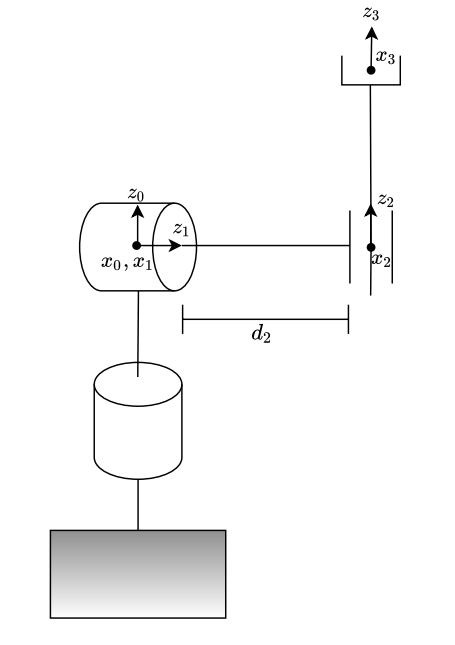
\includegraphics[width=0.75\linewidth]{Fig2_33 Pag 58.png}
\end{minipage}
\hfill
\begin{minipage}[c]{0.45\textwidth}
    \centering
    \begin{tabular}{|c|c|c|c|c|}
        \hline
        \textbf{\# Link} & \(\boldsymbol{\theta}\) & \(\boldsymbol{d}\) & \(\boldsymbol{\alpha}\) & \(\boldsymbol{a}\) \\
        \hline
        1 & \(q_{1}\) & 0 & \(-\frac{\pi}{2}\) & 0 \\
        \hline
        2 & \(q_{2}\) & \(d_{2}\) & \(\frac{\pi}{2}\) & 0 \\
        \hline
        3 & 0 & \(q_{3}\) & 0 & 0 \\
        \hline
    \end{tabular}
\end{minipage}

Le matrici di trasformazione omogenea sono:
\[
    ^{0}\bm{A}_{1}(q_{1}) =
    \begin{bmatrix}
        \cos(q_{1}) & 0 & -\sin(q_{1}) & 0\\
        \sin(q_{1}) & 0 & \cos(q_{1}) & 0\\
        0 & -1 & 0 & 0\\
        0 & 0 & 0 & 1
    \end{bmatrix}
    \qquad\qquad
    ^{1}\bm{A}_{2}(q_{2}) =
    \begin{bmatrix}
        \cos(q_{2}) & 0 & \sin(q_{2}) & 0\\
        \sin(q_{2}) & 0 & -\cos(q_{2}) & 0\\
        0 & 1 & 0 & d_{2}\\
        0 & 0 & 0 & 1
    \end{bmatrix}
\]
\[
    ^{2}\bm{A}_{3}(q_{3}) =
    \begin{bmatrix}
        1 & 0 & 0 & 0\\
        0 & 1 & 0 & 0\\
        0 & 0 & 1 & q_{3}\\
        0 & 0 & 0 & 1
    \end{bmatrix}
\]
E quindi
\[
    ^{0}\bm{T}_{3}(\textbf{q}) \; = \; ^{0}\bm{A}_{1}(q_{1}) \; \cdot \; ^{1}\bm{A}_{2}(q_{2}) \; \cdot \; ^{2}\bm{A}_{3}(q_{3}) =
\]

\[
    =
    \begin{bmatrix}
        c(q_{1})c(q_{2}) & -s(q_{1}) & c(q_{1})s(q_{2}) & c(q_{1})s(q_{2})q_{3} - s(q_{1})d_{2} \\
        s(q_{1})c(q_{2}) & c(q_{1}) & s(q_{1})s(q_{2}) & s(q_{1})s(q_{2})q_{3} + c(q_{1})d_{2}\\
        -s(q_{2}) & 0 & c(q_{2}) & c(q_{2})q_{3}\\
        0 & 0 & 0 & 1
    \end{bmatrix}
\]
% COMBACIA CON CALCOLO MATLAB MANIPOLATORE SFERICO (TIPO II)
\newpage
\subsubsection*{Polso Sferico: Cinematica Diretta}
Il polso sferico è caratterizzato da una configurazione cinematica RRR (\textit{Rotoidale-Rotoidale-Rotoidale}). La denominazione \texttt{Sferico} deriva dal fatto che i tre assi si intersecano in un punto comune, detto \textit{Centro Del Polso}

\begin{minipage}[c]{0.45\textwidth}
    \centering
    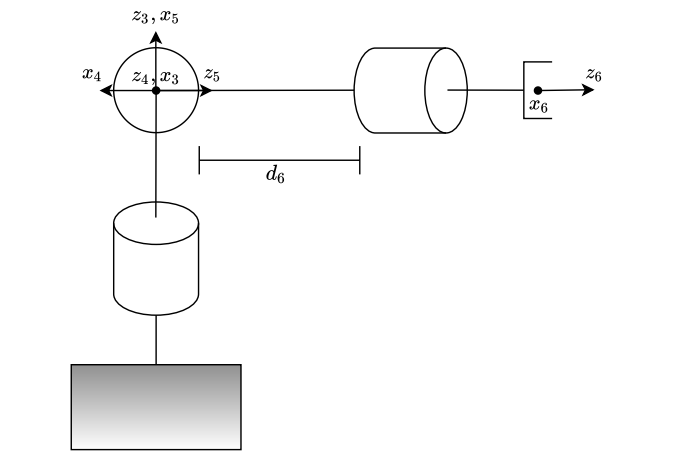
\includegraphics[width=0.9\linewidth]{Fig2_34 Pag 59.png}
\end{minipage}
\hfill
\begin{minipage}[c]{0.45\textwidth}
    % \centering
    \begin{tabular}{|c|c|c|c|c|}
        \hline
        \textbf{\# Link} & \(\boldsymbol{\theta}\) & \(\boldsymbol{d}\) & \(\boldsymbol{\alpha}\) & \(\boldsymbol{a}\) \\
        \hline
        4 & \(q_{4}\) & 0 & \(-\frac{\pi}{2}\) & 0 \\
        \hline
        5 & \(q_{5}\) & 0 & \(\frac{\pi}{2}\) & 0 \\
        \hline
        6 & \(q_{6}\) & \(d_{6}\) & 0 & 0 \\
        \hline
    \end{tabular}
\end{minipage}

Le matrici di trasformazione omogenea sono:
\[
    ^{3}\bm{A}_{4}(q_{4}) =
    \begin{bmatrix}
        \cos(q_{4}) & 0 & -\sin(q_{4}) & 0\\
        \sin(q_{4}) & 0 & \cos(q_{4}) & 0\\
        0 & -1 & 0 & 0\\
        0 & 0 & 0 & 1
    \end{bmatrix}
    \qquad\qquad
    ^{4}\bm{A}_{5}(q_{5}) =
    \begin{bmatrix}
        \cos(q_{5}) & 0 & \sin(q_{5}) & 0\\
        \sin(q_{5}) & 0 & -\cos(q_{5}) & 0\\
        0 & 1 & 0 & 0\\
        0 & 0 & 0 & 1
    \end{bmatrix}
\]
\[
    ^{5}\bm{A}_{6}(q_{6}) =
    \begin{bmatrix}
        \cos(q_{6}) & -\sin(q_{6}) & 0  & 0\\
        \sin(q_{6}) & \cos(q_{6}) & 0 & 0\\
        0 & 0 & 1 & d_{6}\\
        0 & 0 & 0 & 1
    \end{bmatrix}
\]
E quindi
\[
    ^{3}\bm{T}_{6}(\textbf{q}) \; = \; ^{3}\bm{A}_{4}(q_{4}) \; \cdot \; ^{4}\bm{A}_{5}(q_{5}) \; \cdot \; ^{5}\bm{A}_{6}(q_{6}) =
\]

\[
    =
        \begin{bmatrix}
            c(q_{4})c(q_{5})c(q_{6}) - s(q_{4})s(q_{6}) & -c(q_{6})s(q_{4}) - c(q_{4})c(q_{5})s(q_{6}) & c(q_{4})s(q_{5}) & c(q_{4})s(q_{5})d_{6} \\
            c(q_{4})s(q_{6}) + c(q_{5})c(q_{6})s(q_{4}) & c(q_{4})c(q_{6}) - c(q_{5})s(q_{4})s(q_{6}) & s(q_{4})s(q_{5}) & s(q_{4})s(q_{5})d_{6} \\
            -c(q_{6})s(q_{5}) & s(q_{5})s(q_{6}) & c(q_{5}) & c(q_{5})d_{6} \\
            0 & 0 & 0 & 1
        \end{bmatrix}
\]
    % ^{3}\bm{T}_{6} É SICURO GIUSTA COPIATA DA MATLAB
\newpage
\subsubsection*{Manipolatore Di Stanford: Cinematica Diretta}
Poiché, il riferimento \(RF_{3}\) del manipolatore sferico coincide con il riferimento \(RF_{3}\) del polso sferico e di conseguenza la cinematica diretta può essere espressa per composizione delle matrici di trasformazioni

\begin{minipage}[c]{0.4\textwidth}
    \centering
    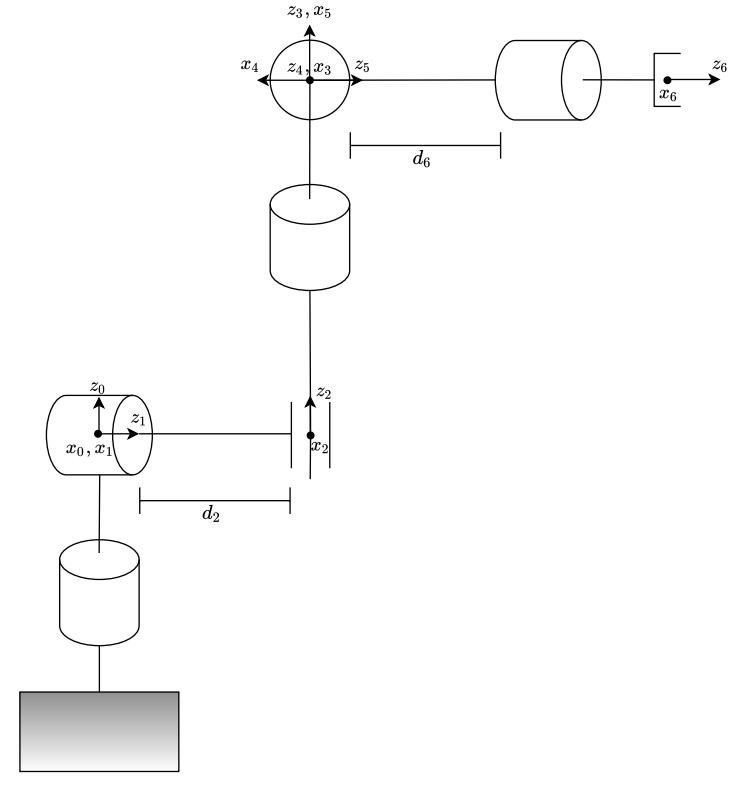
\includegraphics[width=0.99\linewidth]{ManipolatoreStanford.png}
\end{minipage}
\hfill
\begin{minipage}[c]{0.55\textwidth}
    La cinematica diretta del manipolatore completo si ottiene componendo le matrici di trasformazione del braccio e del polso:
    \[
        ^{0}\bm{T}_{6}(\mathbf{q}) \; = \; ^{0}\bm{T}_{3}(\mathbf{q}) \; \cdot \; ^{3}\bm{T}_{6}(\mathbf{q})
    \]
    Il risultato è una matrice di trasformazione omogenea \(4 \times 4\) della forma:
    \[
        ^{0}\bm{T}_{6} =
        \begin{bmatrix}
            \mathbf{A} & \mathbf{B} & \mathbf{C} & \mathbf{D}\\
            0 & 0 & 0 & 1
        \end{bmatrix}
    \]
\end{minipage}

Dove le colonne \(\mathbf{A}\), \(\mathbf{B}\), \(\mathbf{C}\) rappresentano la matrice di rotazione \(^{0}\mathbf{R}_{6}\) e la colonna \(\mathbf{D}\) rappresenta il vettore di posizione \(^{0}\mathbf{p}_{6}\). I loro valori, calcolati simbolicamente, sono i seguenti.

% ---- COLONNA A ----
\[
    \mathbf{A} =
    \begin{bmatrix}
        c(q_{1})c(q_{2})c(q_{4})c(q_{5}) - c(q_{5})s(q_{1})s(q_{4}) - c(q_{1})s(q_{2})s(q_{5})\\
        \\
        c(q_{1})c(q_{5})s(q_{4}) - s(q_{1})s(q_{2})s(q_{5}) + c(q_{2})c(q_{4})c(q_{5})s(q_{1})\\
        \\
        -c(q_{2})s(q_{5}) - c(q_{4})c(q_{5})s(q_{2})
    \end{bmatrix}
\]

% ---- COLONNA B ----
\[
    \mathbf{B} =
    \begin{bmatrix}
        -c(q_{4})s(q_{1}) - c(q_{1})c(q_{2})s(q_{4})\\
        \\
        c(q_{1})c(q_{4}) - c(q_{2})s(q_{1})s(q_{4})\\
        \\
        s(q_{2})s(q_{4})
    \end{bmatrix}
\]

% ---- COLONNA C ----
\[
    \mathbf{C} =
    \begin{bmatrix}
        c(q_{1})c(q_{5})s(q_{2}) - s(q_{1})s(q_{4})s(q_{5}) + c(q_{1})c(q_{2})c(q_{4})s(q_{5})\\
        \\
        c(q_{5})s(q_{1})s(q_{2}) + c(q_{1})s(q_{4})s(q_{5}) + c(q_{2})c(q_{4})s(q_{1})s(q_{5})\\
        \\
        c(q_{2})c(q_{5}) - c(q_{4})s(q_{2})s(q_{5})
    \end{bmatrix}
\]

% ---- COLONNA D ----
\[
    \mathbf{D} =
    \begin{bmatrix}
        d_{2}s(q_{1}) + q_{3}c(q_{1})s(q_{2}) + d_{6}c(q_{1})c(q_{5})s(q_{2}) - d_{6}s(q_{1})s(q_{4})s(q_{5}) + d_{6}c(q_{1})c(q_{2})c(q_{4})s(q_{5})\\
        \\
        q_{3}s(q_{1})s(q_{2}) - d_{2}c(q_{1}) + d_{6}c(q_{5})s(q_{1})s(q_{2}) + d_{6}c(q_{1})s(q_{4})s(q_{5}) + d_{6}c(q_{2})c(q_{4})s(q_{1})s(q_{5})\\
        \\
        q_{3}c(q_{2}) + d_{6}c(q_{2})c(q_{5}) - d_{6}c(q_{4})s(q_{2})s(q_{5})
    \end{bmatrix}
\]
\newpage
\subsubsection{Proprietà di Disaccoppiamento Cinematico}
La struttura del manipolatore di Stanford è progettata per semplificare la risoluzione del problema cinematico inverso grazie a una proprietà nota come \textbf{disaccoppiamento cinematico}. L'obiettivo è determinare le variabili di giunto \(\mathbf{q}\) per raggiungere una posa desiderata, data come matrice di trasformazione omogenea \(^{0}\mathbf{T}_{6}\), che contiene la rotazione \({}^0\mathbf{R}_6\) e la posizione \({}^{0}\mathbf{d}_{6}\) desiderate. Questi due termini sono i \textbf{dati di input noti} del nostro problema, espressi come matrice omogenea:
\[
    ^{0}\mathbf{T}_{6} =
    \begin{bmatrix}
         {}^0\mathbf{R}_6 & {}^{0}\mathbf{d}_{6} \\
         \mathbf{0}_{1 \times 3} & 1
    \end{bmatrix}
\]

La strategia risolutiva consiste nel dividere il problema in due parti:
\begin{enumerate}
    \item \textbf{Cinematica Inversa Di Posizione:} Trovare $(q_1, q_2, q_3)$ per posizionare il \textit{centro del polso}.
    \item \textbf{Cinematica Inversa Di Orientamento:} Trovare $(q_4, q_5, q_6)$ per ottenere l'orientamento finale.
\end{enumerate}

\subsubsection*{Risoluzione Per La Posizione}
Il punto di partenza è l'equazione di posizione che deriva dalla composizione delle trasformazioni \({}^{0}\mathbf{T}_{6} = {}^{0}\mathbf{T}_{3} \cdot {}^{3}\mathbf{T}_{6}\):
\[
    {}^{0}\mathbf{d}_{6} = {}^0\mathbf{R}_3 \, {}^{3}\mathbf{d}_{6} + {}^{0}\mathbf{d}_{3}
\]
Analizziamo i termini di questa equazione nel contesto del problema inverso:
\begin{itemize}
    \item \({}^{0}\mathbf{d}_{6}\): È il \textbf{Vettore Posizione Desiderato} Dell'End-Effector. È un \textbf{dato noto}.
    \item \({}^{0}\mathbf{d}_{3}\) e \({}^0\mathbf{R}_3\): Sono la posizione e l'orientamento del centro del polso. Dipendono solo dai primi tre giunti e sono le \textbf{una delle incognite}.
    \item \({}^{3}\mathbf{d}_{6}\): È la posizione dell'end-effector vista dal centro del polso. Dipende solo dai giunti del polso ed è un'\textbf{altra incognita}.
\end{itemize}
La struttura del polso sferico ci permette di semplificare \({}^{3}\mathbf{d}_{6}\). Questo vettore rappresenta unicamente la traslazione di lunghezza fissa \(d_6\) (un parametro noto del robot) orientata dalla rotazione del polso \({}^3\mathbf{R}_6\):
\[
    {}^{3}\mathbf{d}_{6} = {}^3\mathbf{R}_6
    \begin{bmatrix} 0 \\ 0 \\ d_6 \end{bmatrix}
\]
Sostituendo questa espressione nell'equazione principale e usando la proprietà di composizione delle rotazioni \({}^0\mathbf{R}_6 = {}^0\mathbf{R}_3 \cdot {}^3\mathbf{R}_6\), si ottiene:
\[
    {}^{0}\mathbf{d}_{6} = \underbrace{({}^0\mathbf{R}_3 \cdot {}^3\mathbf{R}_6)}_{{}^0\mathbf{R}_6} \begin{bmatrix} 0 \\ 0 \\ d_6 \end{bmatrix} + {}^{0}\mathbf{d}_{3}
\]
Riordinando l'equazione per isolare le incognite del braccio da un lato e i termini noti dall'altro, si ottiene la formula per la posizione del centro del polso:
\[
    \underbrace{{}^{0}\mathbf{d}_{3}}_{\text{Incognite: } q_1, q_2, q_3} = \underbrace{{}^{0}\mathbf{d}_{6} - {}^0\mathbf{R}_6 \begin{bmatrix} 0 \\ 0 \\ d_6 \end{bmatrix}}_{\text{Termini Noti Dalla Posa Desiderata}}
\]
Il lato destro è ora un vettore numerico calcolabile. Uguagliando questo risultato con l'espressione della cinematica diretta di \({}^{0}\mathbf{d}_{3}\), si possono risolvere $q_1, q_2, q_3$.
\newpage
\subsubsection*{Risoluzione Per L'Orientamento}
Una volta determinati $q_1, q_2, q_3$, la matrice ${}^0\mathbf{R}_3$ è nota. Dalla relazione di composizione delle rotazioni, possiamo calcolare la matrice di rotazione del polso:
\[
    {}^0\mathbf{R}_6 = {}^0\mathbf{R}_3 \cdot {}^3\mathbf{R}_6
\]
Moltiplicando a sinistra per l'inversa di ${}^0\mathbf{R}_3$, che è la sua trasposta $({}^0\mathbf{R}_3)^{T}$, si isola ${}^3\mathbf{R}_6$:
\[
    ({}^0\mathbf{R}_3)^{T} \, {}^0\mathbf{R}_6 = ({}^0\mathbf{R}_3)^{T} \, {}^0\mathbf{R}_3 \, {}^3\mathbf{R}_6
    \qquad\longrightarrow\qquad
    {}^3\mathbf{R}_6 = ({}^0\mathbf{R}_3)^{T} \, {}^0\mathbf{R}_6
\]
Poiché il lato destro è ora una matrice numerica nota, si possono eguagliare i suoi elementi a quelli della matrice cinematica diretta del polso (in funzione di $q_4, q_5, q_6$) per ricavare i valori degli ultimi tre angoli.

\subsubsection{Esempio: Disaccoppiamento Manipolatore Stanford}
%{ SOTTINTESO: Per poter applicare il metodo di disaccoppiamento, dobbiamo prima verificare che il polso soddisfi una specifica condizione matematica. %}
Dai calcoli della cinematica diretta del polso sferico, si è ottenuto:
\[
    ^{3}\mathbf{T}_{6}(\mathbf{q}) =
    \begin{bmatrix}
        c(q_{4})c(q_{5})c(q_{6}) - s(q_{4})s(q_{6}) & -c(q_{6})s(q_{4}) - c(q_{4})c(q_{5})s(q_{6}) & c(q_{4})s(q_{5}) & c(q_{4})s(q_{5})d_{6} \\
        c(q_{4})s(q_{6}) + c(q_{5})c(q_{6})s(q_{4}) & c(q_{4})c(q_{6}) - c(q_{5})s(q_{4})s(q_{6}) & s(q_{4})s(q_{5}) & s(q_{4})s(q_{5})d_{6} \\
        -c(q_{6})s(q_{5}) & s(q_{5})s(q_{6}) & c(q_{5}) & c(q_{5})d_{6} \\
        0 & 0 & 0 & 1
    \end{bmatrix}
\]
Da cui estraiamo il vettore posizione del polso:
\[
    {}^{3}\mathbf{d}_{6} =
    \begin{bmatrix}
        \cos{(q_{4})}\sin{(q_{5})}d_{6}\\
        \sin{(q_{4})}\sin{(q_{5})}d_{6}\\
        \cos{(q_{5})}d_{6}
    \end{bmatrix}
\]
Si deve verificare che esistano due vettori costanti, \(\mathbf{d}_0\) e \(\mathbf{d}_1\), tali che:
\[
    \exists \; \mathbf{d}_{0}, \, \mathbf{d}_{1} \in \mathbb{R}^{3} \; \mid \; {}^{3}\mathbf{d}_{6} = {}^3\mathbf{R}_6 \mathbf{d}_1 + \mathbf{d}_{0}
\]
%{ COMMENTO: d0 rappresenta un offset fisso tra il centro del polso e l'end-effector (una parte che non è influenzata dalle rotazioni), mentre d1 rappresenta la distanza tra il centro del polso e l'origine della terna utensile vista nel sistema di riferimento dell'end-effector (è la lunghezza del link che collega polso e end effector). %}
Si nota che \(\boxed{\mathbf{d}_{0} = \mathbf{0}}\) dato che ogni componente del vettore \({}^{3}\mathbf{d}_{6}\) dipende da almeno una variabile di giunto (\(q_4\) o \(q_5\)) e non ci sono termini costanti di offset. Di conseguenza, la condizione si semplifica in:
\[
    {}^{3}\mathbf{d}_{6} = {}^3\mathbf{R}_6 \mathbf{d}_1
\]
Poiché \({}^3\mathbf{R}_6\) è una matrice di rotazione, la sua inversa è uguale alla sua trasposta, \(({}^3\mathbf{R}_6)^{T} = ({}^3\mathbf{R}_6)^{-1}\). Moltiplicando a sinistra per la trasposta, possiamo isolare \(\mathbf{d}_1\):
\[
   ({}^3\mathbf{R}_6)^{T} \; {}^{3}\mathbf{d}_{6} = ({}^3\mathbf{R}_6)^{T} \; {}^3\mathbf{R}_6 \; \mathbf{d}_1
   \qquad\longrightarrow\qquad
   \boxed{\mathbf{d}_{1} = ({}^3\mathbf{R}_6)^{T} \;  {}^{3}\mathbf{d}_{6}}
\]
Effettuando le sostituzioni si ottiene:
\[
    \mathbf{d}_{1} =
    \begin{bmatrix}
        c(q_{4})c(q_{5})c(q_{6}) - s(q_{4})s(q_{6}) & c(q_{4})s(q_{6}) + c(q_{5})c(q_{6})s(q_{4}) & -c(q_{6})s(q_{5})\\
        -c(q_{6})s(q_{4}) - c(q_{4})c(q_{5})s(q_{6}) & c(q_{4})c(q_{6}) - c(q_{5})s(q_{4})s(q_{6}) & s(q_{5})s(q_{6})\\
        c(q_{4})s(q_{5}) &  s(q_{4})s(q_{5}) &  c(q_{5})
    \end{bmatrix}ù
    \;
    \begin{bmatrix}
        c{q_{4}}s{q_{5}}d_{6}\\
        s{q_{4}}s{q_{5}}d_{6}\\
        c{q_{5}}d_{6}
    \end{bmatrix}
\]
Eseguendo questo prodotto matrice-vettore e applicando le identità trigonometriche fondamentali (es. \(\sin^{2}(\theta) + \cos^{2}(\theta) = 1\)), si ottiene:
\[
    \mathbf{d}_{1} =
    \begin{bmatrix}
        0\\
        0\\
        d_{6}
    \end{bmatrix}
\]
Questo risultato è ammissibile poiché \(\mathbf{d}_1\) è un vettore costante e non dipende dalle variabili di giunto, confermando che la proprietà di disaccoppiamento è valida.

\newpage
\subsubsection*{Cinematica Inversa di Posizione}
Il primo passo è calcolare la posizione numerica desiderata del centro del polso
\[
    {}^{0}\mathbf{d}_{6} = {}^0\mathbf{R}_3 \, {}^{3}\mathbf{d}_{6} + {}^{0}\mathbf{d}_{3} = {}^0\mathbf{R}_3 \, \biggl({}^3\mathbf{R}_6 \cdot \begin{bmatrix} 0\\ 0\\ d_{6} \end{bmatrix}\biggr) + {}^{0}\mathbf{d}_{3}
\]
Ricordando che \({}^{3}\mathbf{d}_{6}\), cioè la posizione dell'origine della terna utensile vista dal centro del polso è data da un offset fisso (lunghezza del link) lungo una direzione opportunamente ruotata a seconda della configurazione del polso e che \({}^0\mathbf{R}_3 \; {}^3\mathbf{R}_6 = {}^0\mathbf{R}_6\)
\[
    {}^{0}\mathbf{d}_{6} = {}^0\mathbf{R}_6 \cdot \underbrace{\begin{bmatrix} 0\\ 0\\ d_{6} \end{bmatrix}}_{= \;\mathbf{d_{1}}} + {}^{0}\mathbf{d}_{3}
\]
Sapendo che \({}^{0}\mathbf{d}_{6}\) e \({}^{0}\mathbf{R}_{6}\) possono essere estratti dalla matrice di trasformazione omogenea \({}^{0}\mathbf{T}_{6}\) e che \(d_{6}\) è un valore noto si può calcolare
\[
    \boxed{
        \hat{{}^{0}\mathbf{d}_{3}} = \underbrace{{}^{0}\mathbf{d}_{6}}_{\text{Noto}} - \underbrace{{}^{0}\mathbf{R}_{6}\mathbf{d}_1}_{\text{Noti}}
    }
\]
%{ COMMENTO: Il lato destro di questa equazione è interamente noto. \hat{d_06} e \hat{R_06} sono l'input del problema, d1 è stato appena calcolato. Il risultato è un vettore numerico 3x1. %}
Ora, eguagliando questo vettore numerico \(\hat{{}^{0}\mathbf{d}_{3}}\) con la sua espressione simbolica, derivata dalla cinematica diretta del manipolatore sferico \({}^{0}\mathbf{T}_{3}\):
\[
    \hat{^{0}\mathbf{d}_{3}} =
    \underbrace{
    \begin{bmatrix}
        c(q_{1})s(q_{2})q_{3} + s(q_{1})d_{2}\\
        s(q_{1})s(q_{2})q_{3} - c(q_{1})d_{2}\\
        c(q_{2})q_{3}
    \end{bmatrix}
    }_{\text{Incognite: } q_1, q_2, q_3}
\]
%{ COMMENTO: Per eliminare $q_1$ e isolare $q_3$, si calcola la norma quadra (prodotto scalare con se stesso) del vettore. %}
Calcolando la norma quadra di entrambi i lati:
\[
    (\hat{^{0}\mathbf{d}_{3}})^{T} (\hat{^{0}\mathbf{d}_{3}}) =
    (c(q_{1})s(q_{2})q_{3} + s(q_{1})d_{2})^2 + (s(q_{1})s(q_{2})q_{3} - c(q_{1})d_{2})^2 + (c(q_{2})q_{3})^2
\]
Svolgendo i calcoli e usando l'identità \(\sin^2\theta + \cos^2\theta = 1\), si ottiene:
\[
    (\hat{^{0}\mathbf{d}_{3}})^{T} (\hat{^{0}\mathbf{d}_{3}}) = d_{2}^{2} + q_{3}^{2}
\]
Da cui, si può isolare \(q_{3}^{2}\):
\[
    q_{3}^{2} = (\hat{^{0}\mathbf{d}_{3}})^{T} (\hat{^{0}\mathbf{d}_{3}}) - d_{2}^{2}
\]
Poiché il giunto \(q_3\) è prismatico, affinché esista una soluzione reale il termine a destra deve essere non negativo (in quanto il valore di questa variabile di giunto è una distanza)
\[
    (\hat{^{0}\mathbf{d}_{3}})^{T} (\hat{^{0}\mathbf{d}_{3}}) - d_{2}^{2} \geq 0
\]
Questa è la \textbf{Condizione Di Raggiungibilità Del Polso}, che assicura che il punto desiderato non sia troppo vicino alla base. Infine, si ottengono due possibili soluzioni per \( q_{3} \):
\[
    \boxed{
        q_{3} = \pm \sqrt{(\hat{^{0}\mathbf{d}_{3}})^{T} (\hat{^{0}\mathbf{d}_{3}}) - d_{2}^{2}}
    }
\]
\newpage
\paragraph{\(\bullet\) Caso \(q_{3} \ne 0\)}: Dalla terza componente del vettore \(\hat{^{0}\mathbf{d}_{3}}\) si ha:
\[
    \hat{^{0}d_{3}}_{z} = q_{3} \cos(q_{2})
\]
%{ $\hat{^{0}d_{3}}_{z}$ è la terza componente (numerica) del vettore $\hat{^{0}\mathbf{d}_{3}}$ calcolato. %}
Si può calcolare \( \cos(q_{2}) \) come:
\[
    \cos(q_{2}) = \frac{\hat{^{0}d_{3}}_{z}}{q_{3}}
\]
Dalla relazione fondamentale \(\sin^{2}(q_{2}) + \cos^{2}(q_{2}) = 1\), si ricava \(\sin(q_{2})\):
\[
    \sin^{2}(q_{2}) = 1 - \cos^{2}(q_{2}) = 1 - \left(\frac{\hat{^{0}d_{3}}_{z}}{q_{3}}\right)^2
    \qquad\longrightarrow\qquad
    \sin(q_{2})  = \pm\sqrt{1 - \left(\frac{\hat{^{0}d_{3}}_{z}}{q_{3}}\right)^2}
\]
L'angolo \(q_2\) si determina univocamente usando la funzione arcotangente a quattro quadranti
\[
    \boxed{q_{2} = \text{atan2} \biggl( \sin(q_{2}), \cos(q_{2}) \biggr)}
\]
La condizione di esistenza per $q_2$ è che il valore di $\cos(q_2)$ sia compreso tra -1 e 1 (\(|\cos(q_2) | \leq 1\) ). Questa porta a \(|\hat{^{0}d_{3}}_{z}| \leq |q_3|\), che si espande in:
\[
    \hat{^{0}d_{3}}_{z}^{2} \leq q_3^2 \quad \longrightarrow \quad \hat{^{0}d_{3}}_{z}^{2} \leq (\hat{^{0}\mathbf{d}_{3}})^{T} (\hat{^{0}\mathbf{d}_{3}}) - d_{2}^{2}
\]
Sostituendo \((\hat{^{0}\mathbf{d}_{3}})^{T} (\hat{^{0}\mathbf{d}_{3}}) = \hat{^{0}d_{3}}_{x}^2 + \hat{^{0}d_{3}}_{y}^2 + \hat{^{0}d_{3}}_{z}^2\), si ottiene:
\[
    \hat{^{0}d_{3}}_{z}^2 \leq \hat{^{0}d_{3}}_{x}^2 + \hat{^{0}d_{3}}_{y}^2 + \hat{^{0}d_{3}}_{z}^2 - d_{2}^{2}
\]
\[
    d_{2}^{2} \leq \hat{^{0}d_{3}}_{x}^2 + \hat{^{0}d_{3}}_{y}^2 + \hat{^{0}d_{3}}_{z}^2 - \hat{^{0}d_{3}}_{z}^2
    \qquad\longrightarrow\qquad
    d_2^2 \leq \hat{^{0}d_{3}}_{x}^2 + \hat{^{0}d_{3}}_{y}^2
\]
Questa condizione significa che la distanza del polso dall'asse \(z_0\) deve essere maggiore o uguale a \(d_2\), il che è geometricamente intuitivo.\\
Per calcolare \(q_{1}\), si considerano le prime due equazioni del sistema:
\[
    \begin{bmatrix}
        \hat{^{0}d_{3}}_{x}\\
        \hat{^{0}d_{3}}_{y}
    \end{bmatrix}
    =
    \begin{bmatrix}
        q_{3}\sin(q_{2}) & d_{2}\\
        -d_{2} & q_{3}\sin(q_{2})
    \end{bmatrix}
    \begin{bmatrix}
        \cos(q_{1})\\
        \sin(q_{1})\\
    \end{bmatrix}
\]
Invertendo la matrice (il cui determinante è \(q_{3}^{2}s^{2}(q_{2}) + d_{2}^{2} \ne 0\) se non si è in una singolarità), si ottiene:
\[
    \begin{bmatrix}
        \cos(q_{1})\\
        \sin(q_{1})\\
    \end{bmatrix}
    =
    \frac{1}{q_{3}^{2}s^{2}(q_{2}) + d_{2}^{2}}
    \begin{bmatrix}
        q_{3}\sin(q_{2}) & -d_{2}\\
        d_{2} & q_{3}\sin(q_{2})
    \end{bmatrix}
    \begin{bmatrix}
        \hat{^{0}d_{3}}_{x}\\
        \hat{^{0}d_{3}}_{y}
    \end{bmatrix}
\]
Da cui si ottengono le espressioni per \(c(q_1)\) e \(s(q_1)\):
\[
    \cos(q_1) = \frac{\hat{^{0}d_{3}}_{x} \; q_3 \; \sin(q_2) - \hat{^{0}d_{3}}_{y} \; d_2}{q_3^2 \; \sin^2(q_2) + d_2^2}
    \quad , \quad
    \sin(q_1) = \frac{\hat{^{0}d_{3}}_{y} \; q_3 \; \sin(q_2) + \hat{^{0}d_{3}}_{x} \; d_2}{q_3^2 \; \sin^2(q_2) + d_2^2}
\]
E infine, \(q_1\) si trova con la funzione \texttt{atan2}:
\[
    \boxed{
        q_{1} = \text{atan2} \biggl( \sin(q_{1}), \cos(q_{1}) \biggr)
    }
\]

\paragraph{\(\bullet\) Caso \(q_{3} = 0\)}:
%{ COMMENTO: Questa è una configurazione singolare in cui il polso si trova sull'asse del secondo giunto. %}
Se \(q_3=0\), l'equazione per la terza componente di \(\hat{^{0}\mathbf{d}_{3}}\) diventa:
\[
    \hat{^{0}d_{3}}_{z} = \cos(q_{2})q_{3} = \cos(q_{2}) \cdot 0 = 0
\]
Il sistema per le altre due componenti si semplifica notevolmente:
\[
    \begin{cases}
        \hat{^{0}d_{3}}_{x} = s(q_{1})d_{2}\\
        \hat{^{0}d_{3}}_{y} = -c(q_{1})d_{2}\\
    \end{cases}
\]
Da cui si può ricavare direttamente \(q_1\):
\[
    \boxed{q_{1} = \text{atan2}( \hat{^{0}d_{3}}_{x}, \;-\hat{^{0}d_{3}}_{y} )}
\]
In questo caso, l'angolo \(q_2\) non appare più nelle equazioni di posizione. Questo significa che le precedenti valgono per qualsiasi valore di \(q_2 \in \mathbb{R}\). Questo significa che \(q_2\) è arbitrario e non influisce sulla posizione del polso. Si ha una ridondanza.

\newpage
\paragraph{\(\bullet\) Caso \(\mathbf{(\hat{^{0}\mathbf{d}_{3}})^{T} (\hat{^{0}\mathbf{d}_{3}}) = d_{2}^{2}}\)}
Questa condizione di singolarità si verifica quando il modulo quadro del vettore posizione è uguale al quadrato della lunghezza del secondo braccio, \(d_2\). Geometricamente, questo implica che il centro del polso si trova sulla superficie di una sfera di raggio \(d_2\), il cui centro è l'origine di \(RF_{1}\). Tale situazione impone un vincolo cinematico che porta il parametro \(q_3\) ad assumere un unico valore, ovvero \(\mathbf{q_3 = 0}\). Di conseguenza, la configurazione del manipolatore acquisisce un grado di libertà aggiuntivo, poiché la variabile di giunto \(q_2\) può assumere un valore arbitrario senza modificare la posizione dell'organo terminale. Per una data posizione, è comunque possibile determinare il valore di \(q_1\) tramite la relazione trigonometrica:
\[
    q_{1} = \text{atan2}(-\hat{d}_{1}, \hat{d}_{2})
\]
A causa della libertà di variazione di \(q_2\), in questa condizione singolare il sistema ammette infinite soluzioni.

\paragraph{\(\bullet\) Caso \(\mathbf{s(q_{2}) = 0}\)}
Questa condizione di singolarità si manifesta quando \(\mathbf{q_2 = 0}\) o \(\mathbf{q_2 = \pi}\), che corrisponde a \(\cos(q_{2}) = \pm 1\). In questa configurazione, il braccio prismatico risulta allineato con l'asse \(z_0\). Dal punto di vista cinematico, ciò causa una dipendenza tra il primo e il terzo giunto per i movimenti sul piano orizzontale, portando a una cinematica degenere. Nonostante la singolarità, è ancora possibile determinare le variabili di giunto. Il calcolo di \(q_3\) rimane invariato e si ottiene dalla seguente relazione:
\[
    q_{3} = \pm \sqrt{(\hat{^{0}\mathbf{d}_{3}})^{T} (\hat{^{0}\mathbf{d}_{3}}) - d_{2}^{2}}
\]
La condizione \(s(q_2)=0\) semplifica le equazioni per la determinazione di \(q_1\). Poiché \(q_3\) può assumere due valori (positivo e negativo, a seconda della direzione di estensione), per ciascuno di essi si ottiene un valore univoco per \(q_1\). Pertanto, in questa configurazione singolare si ottengono esattamente due soluzioni distinte per le variabili articolari del manipolatore.

\newpage
\subsubsection*{Cinematica Inversa Orientamento}

Una volta determinate le variabili di giunto del manipolatore sferico ($q_1, q_2, q_3$), la matrice di rotazione ${}^{0}\mathbf{R}_{3}$ che descrive l'orientamento della terna \(RF_{3}\) rispetto alla base \(RF_{0}\) è nota. L'obiettivo ora è calcolare le variabili del polso sferico ($q_4, q_5, q_6$) per ottenere l'orientamento desiderato dell'end-effector, $\hat{}^{0}\mathbf{R}_{6}$.

La relazione tra le matrici di rotazione è:
\[
    \hat{}^{0}\mathbf{R}_{6} = {}^{0}\mathbf{R}_{3} \cdot {}^{3}\mathbf{R}_{6}
\]
Isolando la matrice di rotazione del polso ${}^{3}\mathbf{R}_{6}$, che contiene le incognite $q_4, q_5, q_6$, si ottiene:
\[
    {}^{3}\mathbf{R}_{6} = ({}^{0}\mathbf{R}_{3})^{T} \cdot \hat{}^{0}\mathbf{R}_{6}
\]
\textit{Nota: La matrice $({}^{0}\mathbf{R}_{3})^{T}$ è l'inversa di ${}^{0}\mathbf{R}_{3}$ poiché le matrici di rotazione sono ortonormali.}

Poiché il lato destro dell'equazione è interamente noto, si può calcolare numericamente la matrice ${}^{3}\mathbf{R}_{6}$. Per semplicità di notazione, la indichiamo come $\bar{\mathbf{R}}$:
\[
    \bar{\mathbf{R}} = {}^{3}\mathbf{R}_{6} =
    \begin{bmatrix}
        \bar{r}_{11} & \bar{r}_{12} & \bar{r}_{13} \\
        \bar{r}_{21} & \bar{r}_{22} & \bar{r}_{23} \\
        \bar{r}_{31} & \bar{r}_{32} & \bar{r}_{33}
    \end{bmatrix}
\]
Ora si può eguagliare questa matrice numerica con la sua espressione simbolica derivata dalla cinematica diretta per estrarre gli angoli.

\paragraph{Calcolo di \(q_5\)}
L'angolo $q_5$ viene calcolato per primo, poiché il suo coseno appare isolato nell'elemento $\bar{r}_{33}$ della matrice.
\[
    \bar{r}_{33} = \cos(q_5)
\]
Da questa relazione, possiamo determinare il seno usando l'identità trigonometrica fondamentale:
\[
    \sin(q_5) = \pm \sqrt{1 - \cos(q_5)^2} = \pm \sqrt{1 - \bar{r}_{33}^2}
\]
Si ottengono due possibili soluzioni per $q_5$, che sono fisicamente distinte. Utilizzando la funzione arcotangente a quattro quadranti, che gestisce correttamente i quadranti, si ha:
\begin{equation}
    \boxed{q_{5} = \text{atan2}(\pm \sqrt{1 - \bar{r}_{33}^2}, \; \bar{r}_{33})}
\end{equation}
Questo porta a due rami di soluzioni per l'intero polso. Per ogni soluzione di $q_5$, si procede al calcolo di $q_4$ e $q_6$.

\paragraph{Caso Non Singolare: $\sin(q_5) \neq 0$}
Questa condizione si verifica quando $\bar{r}_{33} \neq \pm 1$. In questo caso, si può dividere per $s(q_5)$ senza incorrere in una divisione per zero.

\subparagraph{Calcolo Di \(q_4\):}
Dalla terza colonna della matrice ${}^{3}\mathbf{R}_{6}$ simbolica, abbiamo:
\[
    \begin{cases}
        \bar{r}_{13} = \cos(q_{4})\sin(q_{5}) \\
        \bar{r}_{23} = \sin(q_{4})\sin(q_{5})
    \end{cases}
    \qquad\longrightarrow\qquad
    \begin{cases}
        \cos(q_{4}) = \displaystyle{\frac{\bar{r}_{13}}{\sin(q_5)}} \\
        \\
        \sin(q_{4}) = \displaystyle{\frac{\bar{r}_{23}}{\sin(q_5)}}
    \end{cases}
\]
L'angolo $q_{4}$ è quindi univocamente determinato per ogni valore di $s(q_5)$:
\begin{equation}
    \boxed{q_4 = \text{atan2}\biggl( \frac{\bar{r}_{23}}{\sin(q_5)}, \frac{\bar{r}_{13}}{\sin(q_5)} \biggr)}
\end{equation}

\subparagraph{Calcolo Di \(q_6\):}
Analogamente, dalla terza riga della matrice ${}^{3}\mathbf{R}_{6}$ simbolica, abbiamo:
\[
    \begin{cases}
        \bar{r}_{31} = -\cos(q_6)\sin(q_5) \\
        \bar{r}_{32} = \sin(q_6)\sin(q_5)
    \end{cases}
    \qquad\longrightarrow\qquad
    \begin{cases}
        \cos(q_{6}) = \displaystyle{-\frac{\bar{r}_{31}}{\sin(q_5)}} \\
        \\
        \sin(q_{6}) = \displaystyle{\frac{\bar{r}_{32}}{\sin(q_5)}}
    \end{cases}
\]
L'angolo $q_{6}$ è quindi:
\begin{equation}
    \boxed{q_6 = \text{atan2}\biggl( \frac{\bar{r}_{32}}{\sin(q_5)}, -\frac{\bar{r}_{31}}{\sin(q_5)} \biggr)}
\end{equation}

\paragraph{Caso Singolare: $\sin(q_5) = 0$}
Questa condizione, nota come "allineamento del polso", si verifica quando $\bar{r}_{33} = \pm 1$, il che implica $q_5 = k\pi$ con $k \in \mathbb{Z}$. In questa configurazione, gli assi di rotazione dei giunti 4 e 6 diventano paralleli, rendendo impossibile distinguere i loro contributi individuali alla rotazione. Si perde un grado di libertà e appaiono infinite soluzioni.

\subparagraph{\(\bullet\) Caso \(q_5 = 0\):}
In questo caso si ha \(\cos(q_5) = 1\) e \(\sin(q_5) = 0\). Sostituendo questi valori nella matrice ${}^{3}\mathbf{R}_{6}$ simbolica, essa si semplifica notevolmente:
\[
    \bar{\mathbf{R}} =
    \begin{bmatrix}
        c(q_{4})c(q_{6}) - s(q_{4})s(q_{6}) & -c(q_{4})s(q_{6}) - s(q_{4})c(q_{6}) & 0 \\
        s(q_{4})c(q_{6}) + c(q_{4})s(q_{6}) & -s(q_{4})s(q_{6}) + c(q_{4})c(q_{6}) & 0 \\
        0 & 0 & 1
    \end{bmatrix}
    =
    \begin{bmatrix}
        \cos(q_4+q_6) & -\sin(q_4+q_6) & 0 \\
        \sin(q_4+q_6) & \cos(q_4+q_6) & 0 \\
        0 & 0 & 1
    \end{bmatrix}
\]
Le equazioni non permettono di separare $q_4$ e $q_6$, ma solo di calcolare la loro \textbf{somma}. Dagli elementi $\bar{r}_{11}$ e $\bar{r}_{21}$ si ha:
\[
    q_4 + q_6 = \text{atan2}(\bar{r}_{21}, \bar{r}_{11})
\]
In questa singolarità, è possibile scegliere arbitrariamente il valore di una delle due variabili (ad esempio $q_4$) e calcolare l'altra di conseguenza ($q_6 = \text{atan2}(\dots) - q_4$).

\subparagraph{\(\bullet\) Caso \(q_5 = \pi\):}
In questo caso si ha \(\cos(q_5) = -1\) e \(\sin(q_5) = 0\). Sostituendo questi valori nella matrice ${}^{3}\mathbf{R}_{6}$ simbolica, essa si semplifica notevolmente:
\[
    \bar{\mathbf{R}} =
    \begin{bmatrix}
        -\cos(q_4-q_6) & -\sin(q_4-q_6) & 0 \\
        -\sin(q_4-q_6) & \cos(q_4-q_6) & 0 \\
        0 & 0 & -1
    \end{bmatrix}
\]
In questo caso, è possibile determinare solo la \textbf{differenza} tra i due angoli:
\[
    q_4 - q_6 = \text{atan2}(-\bar{r}_{21}, \bar{r}_{22})
\]
Anche in questo caso, esiste un numero infinito di soluzioni.


\newpage
\section{Il Problema Cinematico Inverso}
Il problema della cinematica inversa consiste nel determinare i valori delle variabili di giunto \( q \) che realizzano una determinata posa \( r \). Data la funzione di cinematica diretta \(r = f_{r}(q)\), che mappa lo spazio dei giunti nello spazio operativo, il problema cinematico inverso consiste nel calcolare l'inversa di tale funzione: \(q = f_{r}^{-1}(r)\). A differenza della cinematica diretta, la cui soluzione è sempre unica, la cinematica inversa può avere una soluzione unica, molteplici soluzioni, infinite soluzioni oppure, in alcuni casi, nessuna soluzione. Il numero di soluzioni dipende principalmente dalla relazione tra il numero di gradi di libertà del manipolatore, ovvero il numero di \textit{Variabili Di Giunto} (\(n\)), e la dimensione dello \textit{Spazio Dei Compiti} (\(m\)).

\subsubsection*{\(\bullet\) Caso Non Ridondante ($n = m$)}
In questo scenario, il numero di giunti del robot corrisponde esattamente al numero di variabili necessarie per descrivere il compito. Anche in questa condizione di equilibrio, la natura delle soluzioni può variare significativamente.
\begin{itemize}
    \item \textit{Nessuna Soluzione}: Si verifica quando la posa desiderata si trova al di fuori dello spazio di lavoro del manipolatore, a causa di limiti strutturali o per la presenza di ostacoli.
    \item \textit{Soluzioni Multiple In Numero Finito}: È il caso più comune. Esistono diverse configurazioni dei giunti, dette \textit{posture} (ad esempio "gomito alto" e "gomito basso"), che permettono di raggiungere la stessa posa dell'organo terminale.
    \item \textit{Soluzioni Infinite}: Questa situazione si verifica quando il manipolatore si trova in una \textbf{configurazione singolare}. In questo caso il robot perde alcuni gradi di libertà effettivi, il che può limitare i movimenti in certe direzioni o, consentire movimenti indefiniti di alcuni giunti senza che la posa dell'end-effector cambi.
\end{itemize}

\subsubsection*{\(\bullet\) Caso Ridondante ($n > m$)}
Un manipolatore è definito ridondante quando possiede più gradi di libertà di quelli  necessari per eseguire il compito. La ridondanza offre maggiore versatilità, poiché permette di eseguire compiti secondari come l'evitamento di ostacoli, ma introduce ulteriori complessità nella scelta della soluzione.
\begin{itemize}
    \item \textit{Nessuna Soluzione}: Nonostante i gradi di libertà aggiuntivi, la posa richiesta potrebbe comunque risultare irraggiungibile per vincoli strutturali o ambientali.
    \item \textit{Soluzioni Infinite}: Se una soluzione esiste, ne esistono tipicamente infinite. I gradi di libertà in eccesso possono essere utilizzati per riconfigurare internamente il robot (auto-movimento) mantenendo fissa la posa dell'organo terminale.
    \item \textit{Singolarità Con Soluzioni Finite O Infinite}: Anche i robot ridondanti possono incontrare configurazioni singolari, con conseguente perdita di controllabilità o instabilità nei movimenti.
\end{itemize}


\subsection{Metodi Di Soluzione Numerica}
Quando non è possibile trovare una soluzione in forma chiusa, si ricorre a metodi numerici iterativi. Questi algoritmi partono da una stima iniziale della configurazione del robot e la affinano progressivamente fino a minimizzare l'errore tra la posa raggiunta e quella desiderata. I due approcci principali sono:
\begin{itemize}
    \item \textbf{Metodo Di Newton}: Basato sulla risoluzione di un sistema di equazioni non lineari, implementato attraverso l'inversione (o pseudo-inversione) della matrice Jacobiana del manipolatore.
    \item \textbf{Metodo del Gradiente}: Un algoritmo di ottimizzazione che interpreta il problema come la minimizzazione di una funzione di costo, tipicamente basata sulla distanza tra la configurazione corrente e quella desiderata. L'algoritmo aggiorna le variabili di giunto muovendosi nella direzione di massima discesa del gradiente di tale funzione.
\end{itemize}

\newpage
\subsubsection{Il Metodo Di Newton}
Il metodo di Newton è un metodo numerico che permette di risolvere il problema della cinematica inversa tramite la risoluzione di un sistema di equazioni non lineari. Dalla cinematica diretta sappiamo che la la posa è data dalla funzione
\[
    \bm{r} = f_{r}(\bm{q})
\]
che mappa le variabili di giunto \(\bm{q} \in \mathbb{R}^n\) alla posa dell'end-effector \(\bm{r} \in \mathbb{R}^m\). Quindi possiamo definire un vettore errore \(\bm{e}(\bm{q})\) che descrive la differenza tra la posa desiderata \(\bm{r}\) e quella attuale data dalla cinematica diretta:
\[
    \bm{e}(\bm{q}) = \bm{r} - f_{r}(\bm{q})
\]
Lo scopo dell'algoritmo è annullare questo errore. L'idea fondamentale è quella di vedere il problema come un sistema di controllo e progettare una legge per la velocità dei giunti. Assumendo che la posa desiderata non cambi nel tempo si può dire che la sua derivata sia costante nel tempo (\(\dot{\bm{r}} = \bm{0}\)) e quindi si avrà:
\[
    \dot{\bm{e}}(\bm{q}) = - \frac{\partial f_{r}(\bm{q})}{\partial t}
\]
Usando la regola di derivazione della catena diventa:
\[
    \dot{\bm{e}}(\bm{q}) = -\frac{\partial \bm{f}_r(\bm{q})}{\partial \bm{q}} \frac{d\bm{q}}{dt}
\]
Quindi, l'equazione che lega la dinamica dell'errore alla velocità dei giunti è:
\[
    \boxed{\dot{\bm{e}} = - \underbrace{\bm{J}(\bm{q})}_{\in \mathbb{R}^{m \times n}} \cdot \underbrace{\dot{\bm{q}}}_{\text{Da Progettare}}}
\]
È possibile definire una dinamica per l'errore che sia stabile e convergente a zero.\\
Una scelta comune è
\[
    \dot{\bm{e}} = -\bm{K} \cdot \bm{e}
\]
Dove \(\bm{K}\) è una matrice quadrata definita positiva (ad esempio \(\bm{K} = k\bm{I}\) con \(k>0\)) in modo che l'errore converga asintoticamente a zero.

Uguagliando le due espressioni di \(\dot{\bm{e}}\) si ottiene
\[
    - \bm{J}(\bm{q}) \dot{\bm{q}} = -\bm{K} \bm{e}
    \qquad\longrightarrow\qquad
    \dot{\bm{q}} = \bm{J}^{-1}(\bm{q}) \bm{K} \bm{e}
\]
Questa equazione rappresenta la soluzione in tempo continuo ed è valida nell'ipotesi che la matrice Jacobiana sia quadrata e non singolare, cioè invertibile.


\paragraph{Algoritmo Iterativo Discreto}
Per un'implementazione pratica è necessario discretizzare la legge di controllo continua. Utilizzando il metodo di Eulero esplicito con un passo di integrazione \(T\), l'aggiornamento della configurazione dei giunti ad ogni iterazione \(k\) è dato da:
\[
    \bm{q}_{k+1} = \bm{q}_k + T \cdot \dot{\bm{q}}(\bm{q}_k)
\]
Sostituendo l'espressione di \(\dot{\bm{q}}\) e la definizione dell'errore \(\bm{e}\), si ottiene la formula di aggiornamento iterativa completa:
\[
    \bm{q}_{k+1} = \bm{q}_k + T \cdot \bm{J}^{-1}(\bm{q}_k) \bm{K} \left[ \bm{r} - \bm{f}_r(\bm{q}_k) \right]
\]
La versione classica del \textbf{metodo di Newton-Raphson} per la ricerca di radici di sistemi di equazioni può essere vista come un caso particolare di questa formula, in cui si sceglie un passo di integrazione unitario (\(T=1\)) e un guadagno identitario (\(\bm{K}=\bm{I}\)):
\[
    \bm{q}_{k+1} = \bm{q}_k + \bm{J}^{-1}(\bm{q}_k) \left[ \bm{r} - \bm{f}_r(\bm{q}_k) \right]
\]

\paragraph{Limiti e Gestione Delle Singolarità}
Nonostante la sua efficacia, il metodo di Newton presenta due criticità principali che devono essere considerate:
\begin{itemize}
    \item \textbf{Dipendenza Dalla Stima Iniziale:} La convergenza dell'algoritmo è garantita solo localmente, ovvero se la configurazione iniziale \(\bm{q}_0\) è sufficientemente vicina a una soluzione valida. Se il punto di partenza è troppo lontano, l'algoritmo può divergere o convergere verso una soluzione differente da quella desiderata.
    \item \textbf{Configurazioni Singolari:} Una singolarità cinematica è una configurazione \(\bm{q}\) in cui la matrice Jacobiana \(\bm{J}(\bm{q})\) perde di rango. In queste configurazioni, il manipolatore perde la capacità di muoversi istantaneamente in una o più direzioni dello spazio operativo. L'avvicinarsi a una singolarità causa il mal condizionamento della matrice \(\bm{J}(\bm{q})\), rendendo la sua inversa numericamente instabile. Questo porta a due problemi gravi:
    \begin{enumerate}
        \item L'algoritmo fallisce computazionalmente, poiché il calcolo di \(\bm{J}^{-1}\) è impossibile se \(\det(\bm{J}) \approx 0\).
        \item Le velocità dei giunti calcolate, \(\dot{\bm{q}}\), tendono ad assumere valori estremamente elevati, che sono irrealizzabili per gli attuatori del robot e possono causare movimenti bruschi e potenzialmente dannosi.
    \end{enumerate}
\end{itemize}

\paragraph{Caso Dei Manipolatori Ridondanti}
Quando un manipolatore è ridondante, il numero di giunti è maggiore della dimensione dello spazio dei compiti (\(n > m\)), quindi la matrice Jacobiana \(\bm{J}(\bm{q})\) è una matrice rettangolare (\(m \times n\)) e non è invertibile nel senso classico. Il sistema lineare \(\bm{J}\dot{\bm{q}} = \bm{K}\bm{e}\) ammette infinite soluzioni per \(\dot{\bm{q}}\).

Per selezionare una soluzione univoca, si ricorre alla \textbf{pseudoinversa destra} di Moore-Penrose, definita come:
\[
    \bm{J}^{\#}(\bm{q}) = \bm{J}^T (\bm{J} \bm{J}^T)^{-1}
\]
Questa matrice fornisce la soluzione \(\dot{\bm{q}} = \bm{J}^{\#} \bm{K} \bm{e}\) che, tra tutte le infinite possibili, è quella che minimizza la norma Euclidea \(||\dot{\bm{q}}||\). Dal punto di vista fisico, questa scelta corrisponde alla soluzione che richiede le velocità di giunto istantanee più basse, un criterio spesso desiderabile per minimizzare il consumo energetico e garantire un movimento più fluido.

La formula iterativa per il caso ridondante diventa quindi:
\[
    \bm{q}_{k+1} = \bm{q}_k + T \cdot \bm{J}^{\#}(\bm{q}_k) \bm{K} \left[ \bm{r} - \bm{f}_r(\bm{q}_k) \right]
\]
È importante notare che anche l'approccio con la pseudoinversa fallisce nelle configurazioni singolari, poiché in tali punti la matrice quadrata \(\bm{J}\bm{J}^T\) diventa singolare e quindi non invertibile.

\newpage
\subsubsection{Il Metodo Del Gradiente}
Il metodo del gradiente affronta il problema della cinematica inversa formulandolo come un problema di \textbf{ottimizzazione}. L'obiettivo è quello di trovare la configurazione dei giunti \(\bm{q}\) che minimizza una funzione di costo, che rappresenta l'errore tra la posa desiderata dall'end-effector e quella attuale.

La funzione di costo \(V(\bm{q})\), è comunemente definita come la norma quadratica dell'errore \(\bm{e}\) dato dalla differenza tra la posa desiderata \(\bm{r}\) e la posa attuale, descritta dalla cinematica diretta \(\bm{f}_r(\bm{q})\). La funzione di costo è quindi:
\[
    V(\bm{q}) = \frac{1}{2} \bm{e}^T \bm{e} = \frac{1}{2} \| \bm{r} - \bm{f}_r(\bm{q}) \|^2
\]
Il problema di cinematica inversa si traduce quindi nel definire una legge per la velocità dei giunti, \(\dot{\bm{q}}\), che garantisca una diminuzione progressiva di \(V(\bm{q})\), guidando il sistema verso un minimo della funzione di errore.

Per assicurare che il valore della funzione di costo diminuisca nel tempo, la sua derivata temporale, \(\dot{V}(\bm{q})\), deve essere definita negativa (\(\dot{V} < 0\)). Applicando la regola di derivazione a catena, otteniamo:
\[
    \dot{V}(\bm{q}) = \frac{\partial V(\bm{q})}{\partial \bm{q}} \frac{d\bm{q}}{dt} = \nabla V(\bm{q})^T \dot{\bm{q}}
\]
Il gradiente di \(V(\bm{q})\) rispetto a \(\bm{q}\) viene calcolato applicando la regola di derivazione a catena alla funzione di costo \(V(\bm{q}) = \frac{1}{2} \bm{e}^T \bm{e}\):
\[
    \nabla V(\bm{q})^T = \frac{\partial}{\partial \bm{q}} \left( \frac{1}{2} \bm{e}^T \bm{e} \right) = \bm{e}^T \frac{\partial \bm{e}}{\partial \bm{q}} =
\]
\[
    = \bm{e}^T\frac{\partial}{\partial \bm{q}} \biggl[\bm{r} - \bm{f}_r(\bm{q}) \biggr] = \bm{e}^T \biggl[- \frac{\partial \bm{f}_r(\bm{q})}{\partial \bm{q}} \biggr] = - \bm{e}^T \bm{J}(\bm{q})
\]
Sostituendo il gradiente nell'espressione di \(\dot{V}\), si ottiene:
\[
    \dot{V}(\bm{q}) = - \bm{e}^T \bm{J}(\bm{q}) \dot{\bm{q}}
\]
Per garantire che \(\dot{V} \le 0\), si può scegliere una legge per \(\dot{\bm{q}}\) che si muova nella direzione di massima discesa, ovvero la direzione opposta a quella del gradiente. Questa scelta definisce la \textbf{legge del gradiente}:
\[
    \dot{\bm{q}} = \alpha \, \bm{J}^T(\bm{q}) \bm{e}(\bm{q})
\]
dove \(\alpha > 0\) è un guadagno scalare positivo che regola la velocità di convergenza. Per verificare la stabilità del sistema, sostituiamo questa legge di controllo nell'espressione di \(\dot{V}\):
\[
    \dot{V} = - \bm{e}^T \bm{J} (\alpha \bm{J}^T \bm{e}) = - \alpha (\bm{J}^T \bm{e})^T (\bm{J}^T \bm{e}) = - \alpha \| \bm{J}^T \bm{e} \|^2 \leq 0
\]
Poiché \(\alpha\) è positivo e la norma quadratica è sempre una quantità non negativa, la derivata \(\dot{V}\) risulta semi-definita negativa. Questo garantisce che la funzione di costo non aumenti e, di conseguenza, l'errore di posa si riduca o rimanga costante.

\paragraph{Algoritmo Iterativo Discreto}
Per un'implementazione pratica, la legge di controllo continua viene discretizzata nel tempo. Utilizzando il metodo di Eulero esplicito con un passo di integrazione \(T\), si ottiene una formula di aggiornamento iterativa per la configurazione dei giunti:
\[
    \bm{q}_{k+1} = \bm{q}_k + T \cdot \dot{\bm{q}}(\bm{q}_k)
\]
Sostituendo l'espressione della legge del gradiente, l'algoritmo iterativo diventa:
\[
    \bm{q}_{k+1} = \bm{q}_k + \alpha' \bm{J}^T(\bm{q}_k) \left[ \bm{r} - \bm{f}_r(\bm{q}_k) \right]
\]
dove il nuovo guadagno \(\alpha' = T \cdot \alpha\) è un parametro positivo, spesso chiamato \textit{learning rate}. La scelta di \(\alpha'\) è cruciale, poiché influenza direttamente la stabilità e la velocità di convergenza dell'algoritmo. Un valore troppo grande può rendere il sistema instabile, mentre un valore troppo piccolo può rallentare eccessivamente la convergenza.

\paragraph{Problemi e Limiti: I Minimi Locali}
Il principale svantaggio del metodo del gradiente è la sua suscettibilità ai \textbf{minimi locali}. L'algoritmo arresta la sua esecuzione quando \(\dot{V} = 0\), condizione che si verifica se \(\bm{J}_r^T(\bm{q}) \bm{e}(\bm{q}) = \bm{0}\). Questo avviene certamente quando l'errore è nullo (\(\bm{e}=\bm{0}\)), che corrisponde al minimo globale desiderato. Tuttavia, la condizione può essere soddisfatta anche in configurazioni in cui \(\bm{e} \neq \bm{0}\).

Un minimo locale è una configurazione del robot in cui l'algoritmo si "blocca" prima di aver raggiunto la posa target. In tale punto, qualsiasi piccolo movimento dei giunti provocherebbe un aumento temporaneo della funzione di costo, e il metodo del gradiente, essendo "miope" per sua natura, non è in grado di superare questa "barriera" per proseguire la discesa verso il minimo globale. Questo problema è meno sentito nel metodo di Newton, che mira direttamente ad azzerare la funzione vettoriale \(\bm{e}\) piuttosto che a minimizzarne la norma.

\paragraph{Confronto Con Il Metodo Di Newton}
Di seguito sono riassunte le principali differenze tra i due approcci:
\begin{itemize}
    \item \textbf{Costo Computazionale:} Il metodo del gradiente è significativamente più leggero. Richiede solo il calcolo dello Jacobiano e della sua trasposta (\(\bm{J}_r^T\)), un'operazione computazionalmente quasi irrilevante. Al contrario, il metodo di Newton necessita del calcolo dell'inversa (\(\bm{J}^{-1}\)) o della pseudoinversa (\(\bm{J}^{\#}\)), operazioni molto più onerose.
    \item \textbf{Velocità di Convergenza:} Il metodo di Newton presenta una convergenza di tipo quadratico, che risulta estremamente rapida in prossimità della soluzione. Il metodo del gradiente, invece, ha una convergenza lineare, che è notevolmente più lenta.
    \item \textbf{Robustezza alle Singolarità:} Il metodo del gradiente è intrinsecamente robusto in presenza di singolarità cinematiche. Poiché la matrice trasposta \(\bm{J}_r^T\) esiste sempre ed è ben definita, l'algoritmo non incorre in fallimenti numerici quando \(\det(\bm{J}) \to 0\). In prossimità di una singolarità, la velocità dei giunti calcolata tende semplicemente ad annullarsi, rallentando o arrestando la convergenza ma senza generare instabilità.
\end{itemize}



\end{document}
